\documentclass[11pt,a4paper,notitlepage]{report}
\usepackage[utf8]{inputenc}
\usepackage{amsmath}
\usepackage{amsfonts}
\usepackage{amssymb}
\usepackage{graphicx}
\author{Jan Dziedzic}
\usepackage{fancyhdr}
\usepackage{float}
\usepackage{longtable}
\usepackage[section]{placeins}
\title{PycMan}
\fancypagestyle{}{%
\fancyhf{} % clear all header and footer fields
\fancyhead[RE,LO]{\chaptername \thechapter}
\renewcommand{\headrulewidth}{0pt}
\renewcommand{\footrulewidth}{0pt}
\renewcommand{\chaptername}{Part}}
\newcommand{\dsubsection}[1]{\FloatBarrier \subsection{#1}}
\newenvironment{img}{
	\begin{center}
		\begin{figure}[H]
			\begin{center}
			
}{
	\end{center}
		\end{figure}
			\end{center}
}

\usepackage{listings}
\usepackage{color}

\definecolor{codegreen}{rgb}{0,0.6,0}
\definecolor{codegray}{rgb}{0.5,0.5,0.5}
\definecolor{codepurple}{rgb}{0.58,0,0.82}
\definecolor{backcolour}{rgb}{0.95,0.95,0.92}

\lstdefinestyle{mystyle}{
	backgroundcolor=\color{backcolour},   
	commentstyle=\color{codegreen},
	keywordstyle=\color{magenta},
	numberstyle=\tiny\color{codegray},
	stringstyle=\color{codepurple},
	basicstyle=\footnotesize,
	breakatwhitespace=false,         
	breaklines=true,                 
	captionpos=b,                    
	keepspaces=true,                 
	numbers=left,                    
	numbersep=5pt,                  
	showspaces=false,                
	showstringspaces=false,
	showtabs=false,                  
	tabsize=2
}

\lstset{style=mystyle}




\begin{document}
	\thispagestyle{plain}
	\maketitle
	
	\newpage
	\thispagestyle{empty}
	\newpage
	\thispagestyle{empty}
	\tableofcontents
	\chapter{Project Definition and Analysis}
		\newpage
		\section{Project Definition}
		
			\begin{img}
			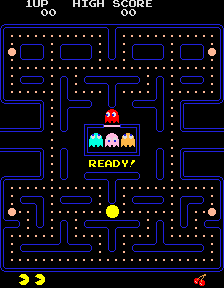
\includegraphics{images/1_1}\\
			\caption{Original Pac-Man screen. Source is Reference \ref{stronaopacmanie}.}
			\label{oryg_pacman}
			\end{img}
		
			As my project, I have decided to present a game written in Python, based around one of its modules - pygame. As I have not had as much time to prepare my project as my colleagues, I have decided that the concept of the game must be simple, yet allowing to demonstrate my programming and computational thinking skills. For this purpose I have decided to mimic the iconic PacMan game.
			For picture of the original game screen please refer to Figure \ref{oryg_pacman}
			
			
		
			Called PycMan (utilizing the fact that many of Python modules have a prefix 'py' in their name), the game itself strongly resembles the original, yet with some meaningful changes. Like in the original - player can move in four directions (left, right, up and down), collecting coins and avoiding ghosts.
			
			
			The game develops critical thinking skills and takes effect of human nature of taking risks and tackling unknown - with having more confidence when predicting ghost behavior, the player actually gets better when playing despite problems generally low complexity.
			
			Actually the game itself may be referred as to playing tag in a transparent maze. Such a play would be very hard for a human to enjoy as analyzing transparent walls while running and predicting opponent's next move is a far too complex problem for human cognition. That's why computational approach on this game is required - where player can see ghosts from above the board whilst ghost may exhibit algorithmically advanced behavior.


		\section{Stakeholders}
			Proposed end user group is really wide. As the game itself can be launched on virtually any device due to Python versatility, it may be used on a spectrum of devices with different controllers, from mobile phones and smart watches through PCs reaching as far as game console emulators mimicking the most authentic PacMan game experience. Such portability should satisfy most users.
			
			The game should grab attention of children - with small challenges that don't require complex thinking and rather promote manual skills and reflex; those who seek quick brainteaser whilst attempting to play with more focus on tactics of ghost avoidance and finally, old gamers who played original PacMan but now they might want to try more modern version with a different approach to critical game mechanisms.
			
			A good example of a stakeholder is my friend, Wojciech Wojtkowski, with whom I have conducted an interview to determine the requirements, see Section \ref{interview} for reference.
		\section{Software Challenges}
			All software used to develop the game but is not necessarily required to run it:
			\begin{itemize}
				\item Python3
				\subitem Pillow module
				\subitem Pygame module
				\item Pycharm Professional
				\item GIMP - GNU Image Manipulation Program
				\item \LaTeX
				\item TeXstudio
				\item LibreOffice Draw
			\end{itemize}
			
			The greatest advantage that convinced me to actually use Python for my game was its portability. As an interpretable programming language, the code of the game remains universal throughout different operating systems and processor architectures. My decision was also influenced by my previous experience with this language and my desire to actually get better around it. It's also free, meaning that everyone can take benefit of my game, without having to buy a license from a third party.
			
			Also, whilst most of my experience was with Python2 I have decided that it's the right time to move on and actually start using Python3, which is reportedly faster and offers more functionality while providing greater stability.
			
			Still, Python does not offer the speed one may expect from a programming language suitable for complex games. Advanced non-optimal solutions need to be thought of and substituted with faster algorithms in order for the game to run smooth on machines lacking processing power.
			
			Happily Python is an objective language - which greatly helped with some designs.
			
			As it's also an interpretable language, it's way easier to debug as one may actually run every single line of code step by step to see variable values changing. Python interpreters also provide a very generous error descriptions greatly helping with bug fixing. 
			
			The closest I could get with Python to making a full featured game conveniently was to use pygame. It's a rather good module supplying some basic functionality one may expect from assisted-design library for creating 2D games. Some functions were not supported out of the box, like level storing (suitable for my purpose) and loading and these had to be implemented by myself as an addition.
			
			Pygame also doesn't have a tiling system I wanted for level designs, to make my game resemble original PacMan in terms of design. I had to write such myself. A similar situation occurred when I wanted to implement discrete "Time Segments" (see Section \ref{timesegments} for reference). For a game such as PacMan I find such solutions to be a very useful optimization and yet these are missing from the pygame module.
			
			Pycharm by JetBrains was used as a Python IDE - it is a really convinient solution and comes with a lot of useful features. It was chosen due to my previous positive experience with it.
			
			GIMP was used to produce graphics resources of the game as well as levels - described later. I found it to be a great deal of overkill for such basic tasks but I am very familiar with it's interface and tools which were of great help especially during the design of semi-transparent ghost graphics.
			
			Libre Office Draw is a free office suite component meant to be used for developing multimedia presentations. I have used it for its great tool for developing flowcharts used in this document. See Figure \ref{segment-part-relation} for example of such graphics.
			
			\LaTeX and Texstudio were used to develop this document. As I identify as a pro-open-source-software person I wanted to use \LaTeX instead of word processors with a far advanced UI, like Microsoft Word. A practical reason behind this - \LaTeX provides an absolutely full flexibility. And even when it doesn't have a function I might want to use - I can always write such myself.
			
			All development was done on an Ubuntu-running computer, therefore	
			I must proudly admit that during the entire design process no non-free software was used. All software was either opensource, freeware or free for education.
			\label{freeware}
			
		\section{The Interview}
			\label{interview}
			To assess interest and gain insight of the potential market for the game, I have interviewed my fellow schoolmate - Wojciech Wojtkowski on his opinion of my approach to redesigning PacMan.
			
			-Hello Wojciech, may I interest you with my Computer Science project - the PycMan, next generation of the classic PacMan with smarter ghosts and different mechanics?
			
			-Sure mate, go ahead!
			
			-Ok, so these are some concept graphics [first two levels were exhibited]...
			
			-...but it looks just like the original!
			
			-Yes, there is a strong resemblance in terms of the graphics, that's what I am aiming for. The biggest difference is how the ghost work.
			
			-Oh, tell me more.
			
			-So, in the classical PacMan, the ghost have their designated area they launch from, A.K.A. "The Ghost House", I want to get rid of that, instead all ghosts will start from predefined locations different for each level.
			
			-That means they will chase you from the exact beginning of the level, isn't that going to make the game harder?
			
			-Yes it will, that is the goal. But that's not the main change. They will be smarter than the originals.
			
			-You mean that the way they move is going to be less predictable?
			
			-That's true, I want to utilize a rather complex algorithm to make them chase player more efficiently.
			
			-Didn't the original have the most efficient solution?
			
			-No, the target machines lacked processing power and memory in the past to actually use that with the game not slowing down. Now, when newer computers are available, I can actually use that.
			
			-So if they were quite stupid then and the game was still hard, won't making them smart render the game impossible to win?
			
			-That's what I am afraid of, I need to find a way to give the player some advantage. Do you, as an experienced gamer, have any idea how to do that?
			
			-I think that making the ghost chase the player indirectly may be the way, how about them tailing the PycMan?
			
			-Yeah, that might be fine but this may eventually lead to them not catching it at all if it doesn't move.
			
			-Oh, that might be the case.
			
			-Actually I have one solution in mind - making them a little bit slower than the player.
			
			-Seems okay, thought I think that one may run away from them, do a risky eating-maneuver then and regain the distance lost. Repeating that will make the game easy and very boring actually.
			
			-Oh, true, I will have to think of these solutions. Probably final version will be designed during beta testing based on player satisfaction with each of these methods.
			
			-Good idea to let the players decide. Actually - on the player-decision thing. One thing that I always wanted with PacMan is to design my own levels. Can you make it possible?
			
			-Yeah, I already have a solution in mind that will make it very easy for anyone to design their own maze, if you say that's going to interest players, I will surely include that.
			
			-Cool! Thanks for letting me know, can I play that game later?
			
			-Of course, as soon as I release the beta.
			
			-Perfect, thank you then, I look forward to playing it.
			
			-Thank you for the talk and insight. Bye.
			
			-Bye.
		\section{Requirement specification (success criteria)}
			For the project to succeed the following criteria must be met:\\
			\begin{enumerate}
				\item 
				The game must resemble the original PacMan in terms of graphical design and some of the mechanics.
				\begin{enumerate}
					\item
						Game graphics should be of similar color and shape to the originals.
						\label{req-orig-colors}
					\item
						Player sprite is an iconic yellow ball with 'mouth'.
						\label{req-player-shape}
					\item
						Player sprite should rotate with 'mouth' towards the direction of movement. 
						\label{req-player-rotation}
					\item
						Neither ghosts nor player are to pass through wall or be able to exit board borders.
						\label{req-walls-not-passable}
					\item
						Ghosts chase the player.
						\label{req-ghost-movement}
					\item
						Player loses a life upon contact with a ghost.
						\label{req-life-loss}
					\item
						Upon losing a life ghosts and the player return to their initial locations.
						\label{req-reset}
					\item
						Each ghost behaves in a different way based on its color.
						\label{req-ghost-differences}
					\item
						Ghosts do not reverse their direction of movement.
						\label{req-ghost-not-reversing}
					\item
						Player progresses through a level with eating 'coins' left throughout some/all accessible places on the map.
						\label{req-level-progress}
					\item
						Upon eating a coin, it disappears and is not to be rendered again.
						\label{req-coins-disappearing}
					\item
						Eating a coin increases point counter.
						\label{req-point++}
					\item
						Heart shaped Eatables are left in some places in some of the levels.
						\label{req-hearts}
					\item
						Eating a heart grants the player extra one life.
						\label{req-lifes++}
					\item
						Upon completing the level (eating all 'coins') new level is loaded.
						\label{req-level-up}
					\item
						When player has less than one life the game finishes and the player loses.
						\label{req-game-over}
					\item
						When player completes all the levels, the game finishes and the player wins.
						\label{req-win}
					\item
						Text messages appear whenever a significant change in gameplay is to take place.
						E.g. Start of the game, level change, player's death, completing entire game.
						\label{req-messages}
					\item
						The game must be possible to win.
						\label{req-winnable}
				\end{enumerate}
				\item
					The game must be different from the original in these ways:
					\begin{enumerate}
						\item
							Majority of players must find the PycMan ghosts 'smarter' than the originals.
							\label{req-smarter-ghosts}
						\item
							There is no 'ghost house' where ghosts start from. All sprites move from the beginning and ghost chase the player immediately.
							\label{req-no-ghost-house}
						\item
							There are no power-ups in the levels.
							\label{req-no-powerips}
						\item
							Ghosts cannot die.
							\label{req-not-dying}
						\item
							Ghost don't change 'modes' and don't became frightened of the player.
							\label{req-no-ghost-modes}
						\item
							Player can move faster than the ghosts.
							\label{req-player-faster}
					\end{enumerate}
				\item 
					Requirements independent from similarities to the original Pac-Man
					\begin{enumerate}
						\item
							Arrow keys used to control player's movement.
							\label{req-input}
						\item
							Spacebar used to dismiss on-screen messages.
							\label{req-spacebar}
						\item
							Player sprite must not move without user input.
							\label{req-player-only-input}
						
					\end{enumerate} 
				\item
					Game must work smoothly (30 frames per second is considered to be the standard of human perception of fluency) on contemporary medium-class laptop PCs. The following hardware and software requirements are to be met:
					\begin{enumerate}
						\item
							Operating system supporting Python3 interpreter
						\item
							Python3 interpreter
						\item
							Pillow module (PIL)
						\item
							Pygame module
						\item
							Color display of resolution of at least 600x600px
						\item
							Keyboard
						\item
							500 MB of storage space
						\item
							512 MB of RAM
						\item
							700MHz processor
					\end{enumerate}
					The game has been tested on described specification machine and has been found to meet fluency criteria. No testing on slower machines has been performed as these are not usually available on the market anymore. Each of the requirements listed is critical to either launch or play the game.
			\end{enumerate}
			
	\chapter{Design}
		\newpage
		As the game uses Pygame module it obviously derives some solutions natively implemented in it. All display solutions are actually handled using the module. Use of Tkinker was researched for pop-up messages but adding another module that doesn't bring any outstanding functionality above capabilities of Pygame has been ruled as an unnecessary waste of memory.
		
		Having the fact that my main tool will be the pygame module I have divided game design process into following subproblems.
		\begin{itemize}
			\item
				Preparing window environment for the game
			\item
				Preparing board and tiling system
			\item
				Creating player and ghost sprites
			\item
				Handling player input
			\item
				Adding Eatables and walls
			\item
				Preparing level storage-loading system
			\item
				Wall collision handling
			\item
				Eating routines
			\item
				Ghost movement system
			\item
				Advancing through levels
			\item
				Pop-up messaging
		\end{itemize}
		\section{Main window layout}
			\begin{img}
				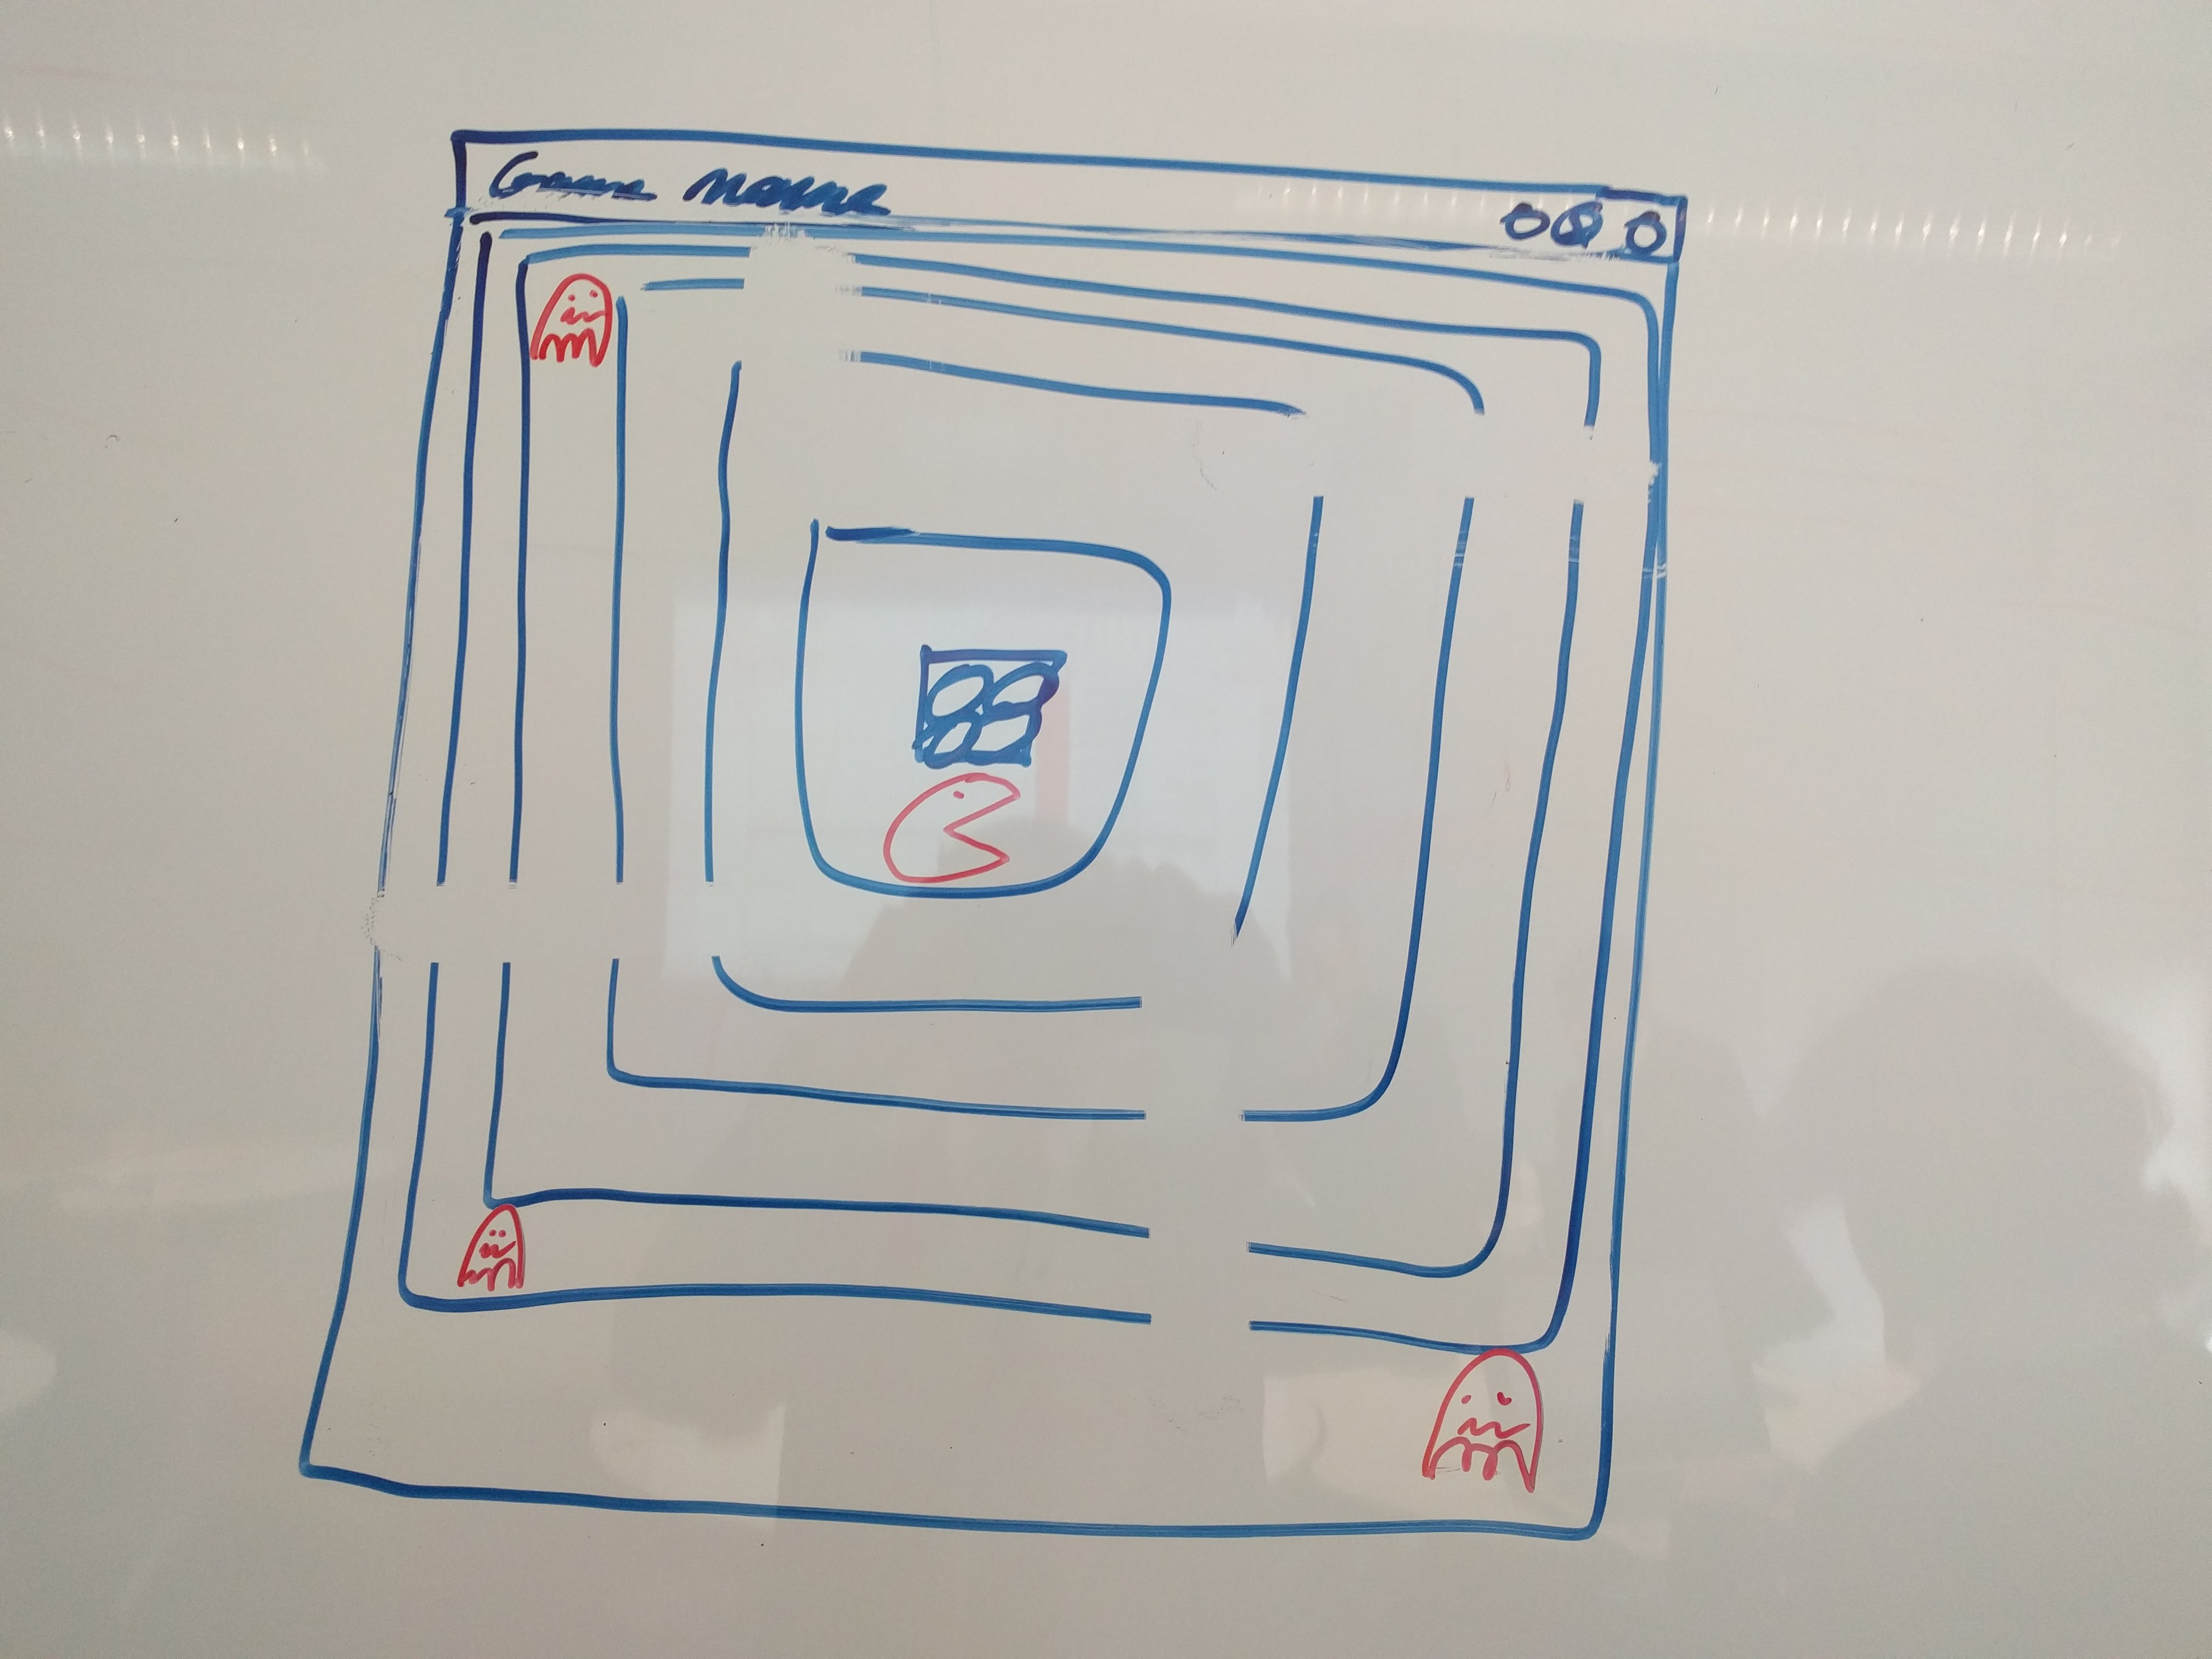
\includegraphics[width=350pt]{images/window_whiteboard.jpg}\\
				\caption{Very early design of the game window. Note the lack of counters.}
			\end{img}
			Main game window consists of a board where the actual game takes place.
			Below the board there is a set of informative counters kept in characteristic PacMan colours of gold-yellow on dark/royal-blue background as per requirement \ref{req-orig-colors}.
			\begin{img}
				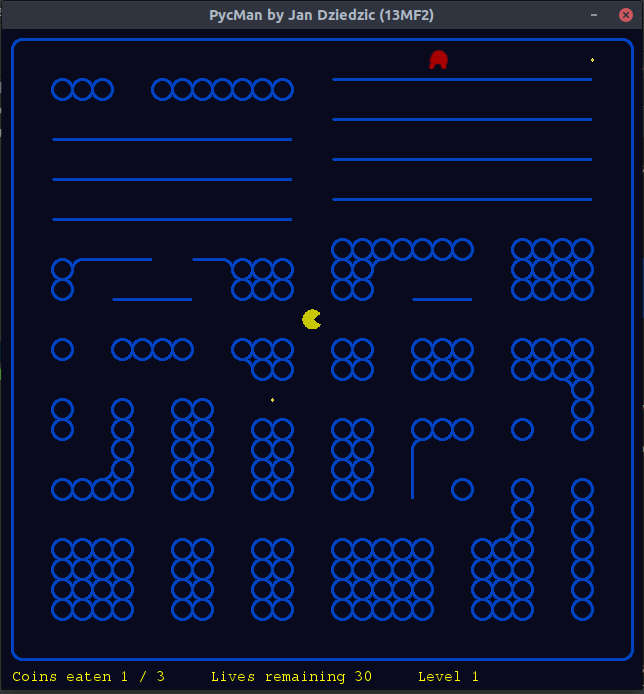
\includegraphics[width=350pt]{images/window-in-ubuntu}\\
				\caption{Game window rendered in Ubuntu Gnome graphical environment.}
			\end{img}
			
			\dsubsection{Board}
				As each level has a different layout so look of the board may vary. Please refer to Figure \ref{example_board} for an example of such board.
				\begin{img}
					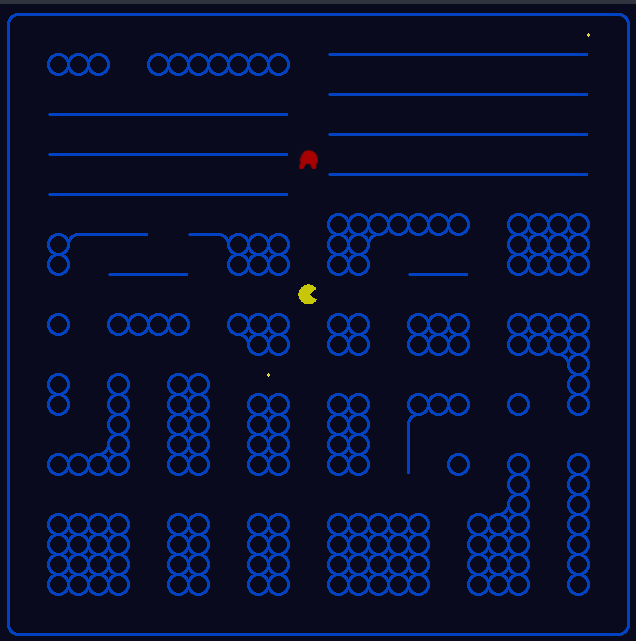
\includegraphics[width=350pt]{images/board_example}\\
					\caption{Example board. Walls, empty tiles, the player, coins and a red ghost are visible}
					\label{example_board}
				\end{img}
				General idea is that all border tiles of each level (tile system explained later) have to be walls, which creates a nice, outer border of the board with rounded edges.
			\dsubsection{Counters}
				\begin{img}
					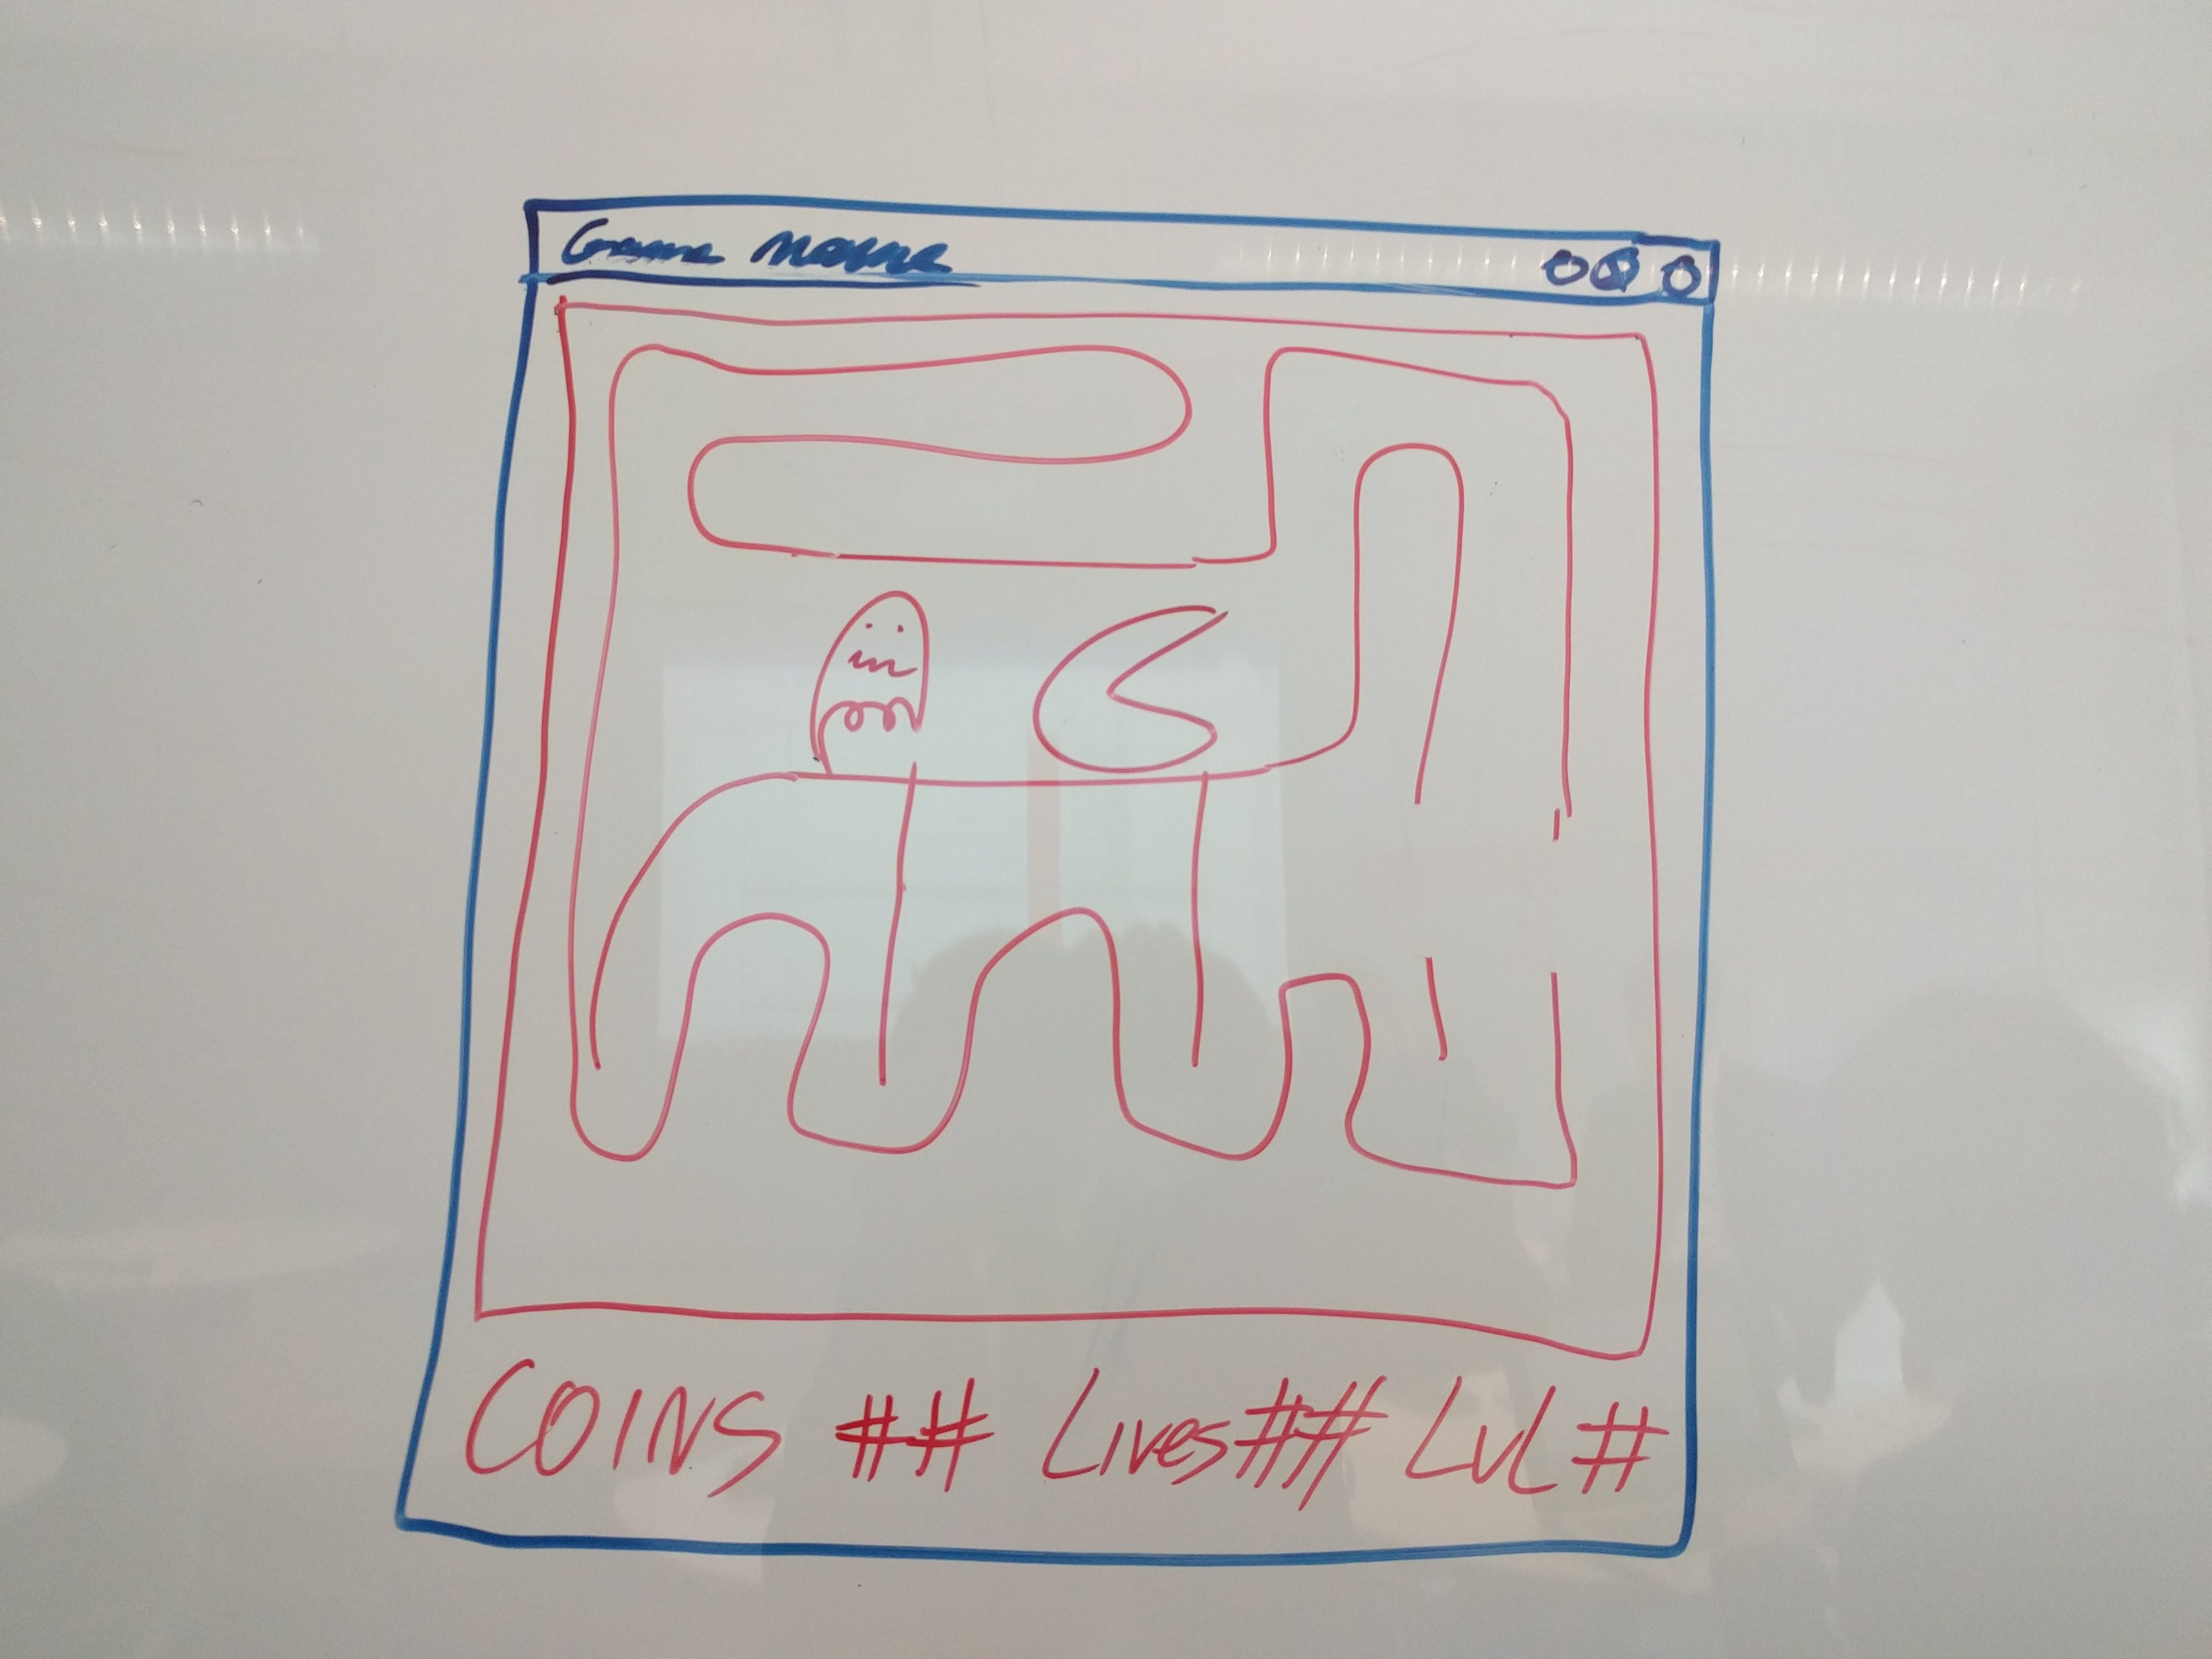
\includegraphics[width=350pt]{images/counters_whiteboard.jpg}\\
					\caption{Counter placement design in its earliest stage.}
				\end{img}
				Directly below the board, counters are located, these provide information on:
				\begin{enumerate}
					\item
						Number of coins eaten
					\item
						Number of coins that are required to be consumed before progressing to the next level
					\item
						Number of player lives
					\item
						Current level number
				\end{enumerate}
				\begin{img}
					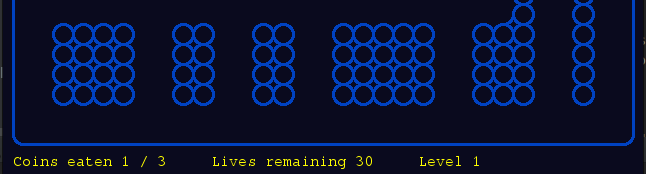
\includegraphics[width=350pt]{images/counter_example}\\
					\caption{Example set of counters with part of the board included for position reference.}
				\end{img}
				Every time the player eats a 'coin' the first counter increases. Throughout the level, this counter cannot decrease as even upon player's death, the already-eaten coins don't respawn.
				
				Number of coins required to progress is constant through the level but may differ between levels. It is worth mentioning that as every coin must be eaten to progress, this acts as a total number of coins allocated in each level map. Coin placing algorithm described later in this document also proves that it equals to $32^2-\#_{wall\_tiles}-\#_{empty\_ tiles}$.
				
				Each time a player comes in contact with a ghost(defined later in this document) a life is subtracted and every time the player eats a heart eatable, a life is added.
				
				Level number increases from 1 (easiest level) up to ten (hardest level), as player advances through the levels.
		\section{Grid layout}
			\label{grid}
			Pygame provides a sprite attribute of its location but as I have decided to use a window of over 500x500px of size, its pixel-accurate positioning would be an overkill and could make programming harder as well as require more processing power to (later mentioned) pathfinding algorithms.
			Due to this I have turned to the original PacMan solution (as read in Reference \ref{stronaopacmanie}), the grid system.
			\begin{img}
				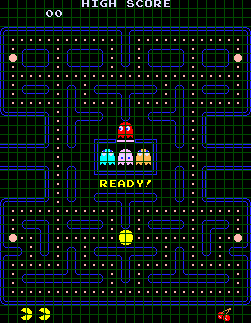
\includegraphics[width=350pt]{images/oryginal_pacman_grid}\\
				\caption{Original Pac-Man with grid layout depicted. Source: Reference \ref{stronaopacmanie}}
			\end{img}
			The PycMan board was initially made as a 64x64 grid, where each piece, namely a tile, was either a wall or a space a sprite may move on. First levels were designed this way and I found the level design a really hard task. Only later I have noticed that the grid of the original PacMan was barely $\dfrac{1}{4}^{\text{th}}$ of the size I have used, my board was just to big for a pleasant gameplay.
			
			As I wanted the board to be square I have decided to move to 32x32 grid. Some testing later I have decided that this size not only nicely divides by 2 making perfectly symmetrical or even fractal levels possible to make but also is actually quite the one most similar in terms of number of tiles to the one the original PacMan had (for square boards).
			\begin{img}
				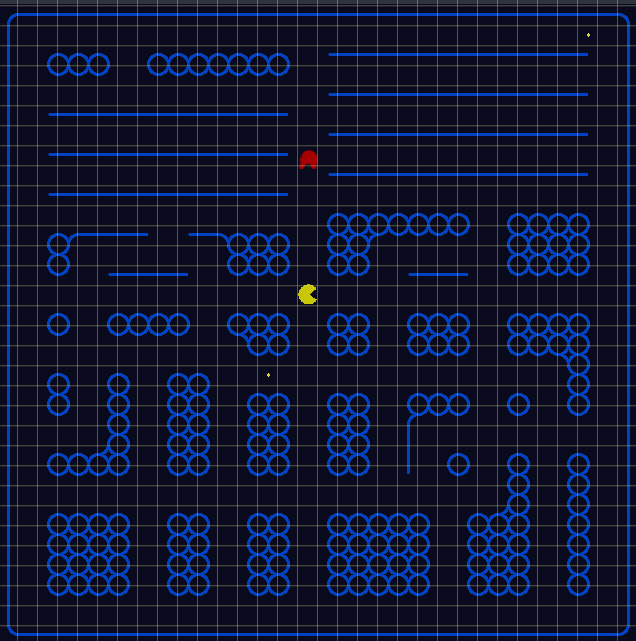
\includegraphics[width=350pt]{images/board_grid}\\
				\caption{Example of a board with a grid applied (note that the grid was added just for demonstrative purposes and in not a part of the game.)}
			\end{img}
			The following section describes types of different tiles used throughout the game.
		\section{Types of tiles}
			\dsubsection{Walls}
				\label{walls}
				As wall tiles have to connect with neighboring (common edge) tiles, they need to be represented by different graphics depending on their surroundings. 
				There is a total of 15 graphics depicted below. The system of numbering them is really intuitive, it consists of four digits each of which is either zero or one
				
				\begin{img}
					\frame{
\includegraphics{images/w0001}}\\
					\caption{Wall 0001}
				\end{img}
				\begin{img}
					\frame{
\includegraphics{images/w0010}}\\
					\caption{Wall 0010}
				\end{img}
				\begin{img}
					\frame{
\includegraphics{images/w0011}}\\
					\caption{Wall 0011}
				\end{img}
				\begin{img}
					\frame{
\includegraphics{images/w0100}}\\
					\caption{Wall 0100}
				\end{img}
				\begin{img}
					\frame{
\includegraphics{images/w0101}}\\
					\caption{Wall 0101}
				\end{img}
				\begin{img}
					\frame{
\includegraphics{images/w0110}}\\
					\caption{Wall 0110}
				\end{img}
				\begin{img}
					\frame{
\includegraphics{images/w0111}}\\
					\caption{Wall 0111}
				\end{img}
				\begin{img}
					\frame{
\includegraphics{images/w1001}}\\
					\caption{Wall 1001}
				\end{img}
				\begin{img}
					\frame{
\includegraphics{images/w1010}}\\
					\caption{Wall 1010}
				\end{img}
				\begin{img}
					\frame{
\includegraphics{images/w1011}}\\
					\caption{Wall 1011}
				\end{img}
				\begin{img}
					\frame{
\includegraphics{images/w1100}}\\
					\caption{Wall 1100}
				\end{img}
				\begin{img}
					\frame{
\includegraphics{images/w1101}}\\
					\caption{Wall 1101}
				\end{img}
				\begin{img}
					\frame{
\includegraphics{images/w1110}}\\
					\caption{Wall 1110}
				\end{img}
				\begin{img}
					\frame{
\includegraphics{images/w1111}}\\
					\caption{Wall 1111}
				\end{img}
				
			
				The first bit represents whether connection is to be made on the right, second whether on the top, third whether on the left and fourth whether on the bottom. As wall 0000 would be very small and hard to maneuver around for user, drawing of such is unsupported. I have actually tested moving around such and even my manual and keyboard skills are relatively good, I found it hard to move around such.
				
				Algorithm deciding which type of wall is presented below:
				\label{walltypecheck}
				\begin{lstlisting} [language=Python]
def walltypecheck(location):
	r = t = l = b = 0
	# note that letters correspond to Right Top Left Bottom
	if location[0] != 0:
		if level[location[0]-1][location[1]] == wall:
			l = 1
	if location[0] != 31:
		if level[location[0]+1][location[1]] == wall:
			r = 1
	if location[1] != 0:
		if level[location[0]][location[1]-1] == wall:
		t = 1
	if location[1] != 31:
		if level[location[0]][location[1]+1] == wall:
			b = 1
	return str(r) + str(t) + str(l) + str(b)
				\end{lstlisting}
				For reference of how level data is stored see section \ref{Levels}.
				This algorithm returns type of wall that would fit in the spot location provided as an argument while calling the function. Output format is a string corresponding with wall names described above.
			\dsubsection{Player}
				Player is represented by an iconic PacMan figure of my own design (to avoid direct copying of work of others). The tile rotates depending on the direction of player's movement so that the 'mouth' is always facing forward as per requirement \ref{req-player-rotation}. Color has been slightly darkened as I find this design a little bit nicer than the original while still complying with requirement \ref{req-player-shape}. 
				\begin{img}
					
\includegraphics{images/player}\\
				\caption{Player sprite}
				\end{img}
			\dsubsection{Ghosts}
				There are three types of ghosts in the game, red, green and blue. They are similar in design, though they behavior is different. (described later)
				 \begin{img}
				 	
\includegraphics{images/redghost}\\
				 	\caption{Red ghost sprite}
				 	\label{ghostimage}
				 \end{img}
				  \begin{img}
				 	
\includegraphics{images/greenghost}\\
				 	\caption{Green ghost sprite}
				 \end{img}
				 \begin{img}
				 	
\includegraphics{images/blueghost}\\
				 	\caption{Blue ghost sprite}
				 \end{img}
			\dsubsection{Eatables}
				\subsubsection{Coins}
					\label{coins}
					Coin spawning works a little bit different than spawning other tiles, which is described later. They actually appear in every tile \textbf{not} designated as 'wall', 'heart' or 'empty'. They are static and their sprites are killed when player enters their tile resulting in coins-eaten counter value increasing.
					\begin{img}
						
\includegraphics{images/coin}\\
						\caption{Coin graphics}
					\end{img}
				\subsubsection{Hearts}
					\label{hearts}
					Hearts are similar to coins in terms of being eaten, but they spawn in designated places and their consumption increases lives counter.
					\begin{img}
						
\includegraphics{images/heart}\\
						\caption{Heart graphics}
					\end{img}
			\dsubsection{Empty tiles}
				These tiles are actually not drawn. They only act as an abstract concept to hold information that coin is not to be drawn on this particular grid tile. Player and ghost can move through this tile. For user these appear as plain dark blue space - the color of the background.
		\section{Levels}
		\label{Levels}
			\dsubsection{Permanent storing}
				\label{level-permanent-storing}
				It took me a while to actually figure out how to store level blueprints. The container had to be a 32x32 matrix of values. Python lists of lists of variables would actually be the most efficient way to store types of tiles on each position in the grid. I have actually tried this approach back when my original board was still 64x64 tiles and it didn't take me 10 tiles of brackets and commas to figure out, that maybe this approach is most efficient for storing, but it is absolutely to slow to prepare the level of 4096 tiles. I have decided that I need an editing software for these grids. Then I understood that my levels, grids of values are actually bitmaps. I have prepared an exemplar of a level in GIMP and using my previous experience with Pillow module I have prepared a script to load these bitmaps to my Python program. It all took less time that it would take to fill $\dfrac{1}{10}^{\text{th}}$ of that list of lists of values manually.
				\begin{img}
					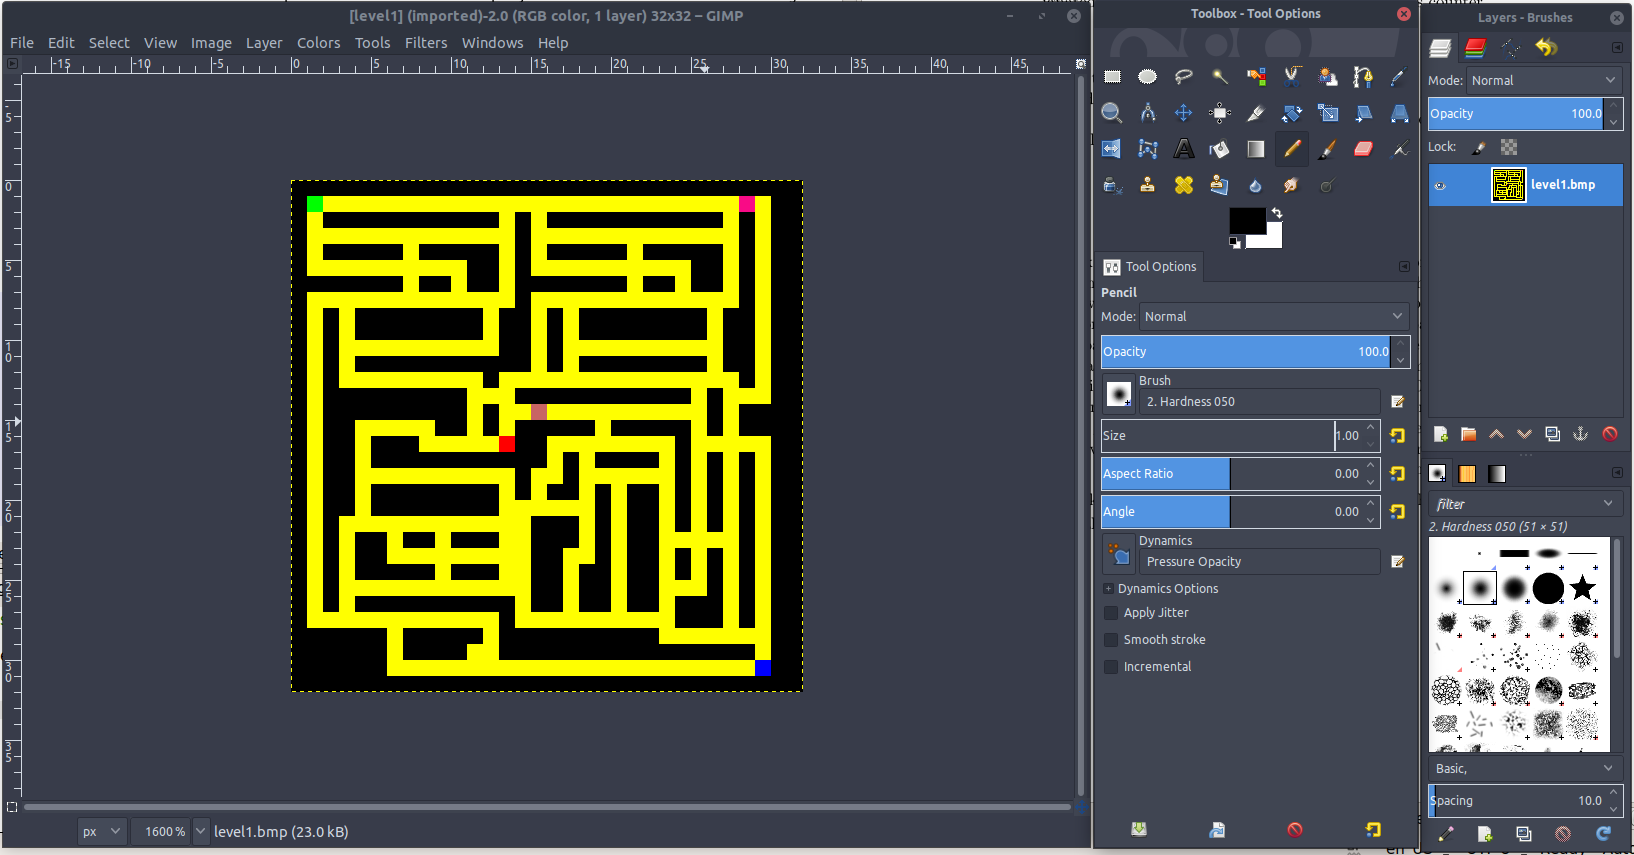
\includegraphics[width=350pt]{images/gimp_level_editing}\\
					\caption{An exemplar of a level being edited in the GIMP software}
					\label{gimplevel}
				\end{img}
				Each tile has its representation in a particular color in RGB notation:\\ \\
				\begin{tabular}{| l | r |}
					\hline 
					Empty tile & (255, 255, 255) \\ \hline
					Wall & (0, 0, 0) \\ \hline
					Coin & (255, 255, 0) \\ \hline
					Player & (255, 0, 0) \\ \hline
					Red Ghost & (200, 100, 100) \\ \hline
					Green Ghost & (0, 255, 0) \\ \hline
					Blue Ghost & (0, 0, 255) \\ \hline
					Heart & (200, 200, 255) \\
					\hline
				\end{tabular}
			\newpage
			\dsubsection{Storing while in game}
				\label{level-ingame-storing}
				Do you remember my first concept for the most optimal storage of levels mentioned earlier? Well, that didn't work for storing levels as files... But in game while loaded in RAM - works like a charm. List of lists of integers, just like that:\\
				\noindent
				\begin{center}
					\begin{small}
					 [[1, 1, 1, 1, 1, 1, 1, 1, 1, 1, 1, 1, 1, 1, 1, 1, 1, 1, 1, 1, 1, 1, 1, 1, 1, 1, 1, 1, 1, 1, 1, 1], \\ [0pt] 
					 [1, 0, 0, 0, 0, 0, 0, 0, 0, 0, 0, 0, 0, 0, 0, 0, 0, 0, 0, 0, 0, 0, 0, 0, 0, 0, 0, 0, 0, 0, 0, 1], \\ [0pt] 
					 [1, 0, 1, 1, 0, 1, 0, 1, 0, 1, 0, 1, 1, 1, 0, 1, 1, 0, 1, 1, 1, 0, 1, 1, 0, 1, 1, 1, 1, 1, 0, 1], \\ [0pt] 
					 [1, 0, 1, 1, 0, 1, 0, 1, 0, 1, 0, 1, 1, 1, 0, 1, 1, 0, 1, 1, 1, 0, 1, 1, 0, 1, 1, 1, 1, 1, 0, 1], \\ [0pt] 
					 [1, 0, 1, 1, 0, 1, 0, 1, 0, 1, 0, 1, 0, 0, 0, 0, 0, 0, 0, 0, 0, 0, 1, 1, 0, 1, 1, 1, 1, 1, 0, 1], \\ [0pt] 
					 [1, 0, 1, 1, 0, 1, 0, 1, 0, 1, 0, 1, 0, 1, 0, 1, 1, 0, 1, 1, 1, 1, 1, 1, 0, 1, 1, 1, 1, 1, 0, 1], \\ [0pt] 
					 [1, 0, 0, 0, 0, 1, 0, 1, 0, 1, 0, 1, 0, 1, 0, 1, 1, 0, 1, 1, 1, 1, 1, 1, 0, 1, 1, 1, 1, 1, 0, 1], \\ [0pt] 
					 [1, 0, 1, 1, 0, 1, 0, 1, 0, 1, 0, 1, 0, 1, 0, 1, 1, 0, 0, 0, 0, 0, 0, 0, 0, 0, 0, 0, 0, 0, 0, 1], \\ [0pt] 
					 [1, 0, 1, 1, 0, 1, 0, 1, 0, 1, 0, 0, 0, 1, 0, 1, 1, 0, 1, 1, 1, 1, 1, 1, 0, 1, 1, 1, 1, 1, 0, 1], \\ [0pt] 
					 [1, 0, 1, 1, 0, 1, 0, 1, 0, 1, 0, 1, 0, 1, 0, 1, 1, 0, 1, 1, 1, 1, 1, 1, 0, 1, 1, 1, 1, 1, 0, 1], \\ [0pt] 
					 [1, 0, 1, 1, 0, 1, 0, 1, 0, 1, 0, 1, 0, 0, 0, 0, 0, 0, 1, 1, 1, 1, 1, 1, 0, 1, 1, 1, 1, 1, 0, 1], \\ [0pt] 
					 [1, 0, 1, 1, 0, 1, 0, 1, 0, 1, 0, 1, 1, 1, 0, 1, 1, 0, 0, 0, 0, 0, 0, 0, 0, 0, 0, 0, 0, 0, 0, 1], \\ [0pt] 
					 [1, 0, 1, 1, 0, 1, 0, 1, 0, 1, 0, 1, 1, 1, 0, 1, 1, 1, 0, 1, 1, 1, 1, 1, 0, 1, 1, 1, 1, 1, 0, 1], \\ [0pt] 
					 [1, 0, 1, 1, 0, 1, 0, 1, 0, 1, 0, 1, 1, 1, 0, 1, 1, 1, 2, 1, 1, 1, 1, 1, 0, 1, 1, 1, 1, 1, 0, 1], \\ [0pt] 
					 [1, 0, 1, 1, 0, 1, 0, 1, 0, 1, 0, 1, 1, 1, 0, 1, 1, 1, 0, 1, 1, 1, 1, 1, 0, 1, 1, 1, 1, 1, 0, 1], \\ [0pt] 
					 [1, 0, 0, 0, 0, 0, 0, 0, 0, 0, 0, 0, 0, 0, 3, 0, 0, 0, 0, 0, 0, 0, 0, 0, 0, 0, 0, 0, 0, 0, 0, 1], \\ [0pt] 
					 [1, 0, 1, 0, 1, 0, 1, 0, 1, 0, 1, 1, 1, 1, 0, 1, 1, 1, 0, 1, 1, 1, 1, 1, 0, 1, 1, 1, 1, 1, 0, 1], \\ [0pt] 
					 [1, 0, 1, 0, 1, 0, 1, 0, 1, 0, 1, 1, 1, 1, 0, 1, 1, 1, 0, 1, 1, 1, 1, 1, 0, 1, 1, 1, 1, 1, 0, 1], \\ [0pt] 
					 [1, 0, 1, 0, 1, 0, 1, 0, 1, 0, 1, 1, 1, 1, 0, 1, 1, 1, 0, 1, 1, 1, 1, 1, 0, 1, 1, 1, 1, 1, 0, 1], \\ [0pt] 
					 [1, 0, 1, 0, 1, 0, 1, 0, 1, 0, 1, 1, 0, 0, 0, 0, 0, 0, 0, 0, 0, 0, 0, 0, 0, 1, 1, 1, 1, 1, 0, 1], \\ [0pt] 
					 [1, 0, 1, 0, 1, 0, 1, 0, 1, 0, 1, 1, 0, 1, 0, 1, 1, 1, 0, 1, 1, 1, 1, 1, 0, 1, 1, 1, 1, 1, 0, 1], \\ [0pt] 
					 [1, 0, 1, 0, 1, 0, 1, 0, 1, 0, 1, 1, 0, 1, 0, 1, 1, 1, 0, 1, 1, 0, 0, 0, 0, 1, 1, 1, 1, 1, 0, 1], \\ [0pt] 
					 [1, 0, 1, 0, 1, 0, 1, 0, 1, 0, 1, 1, 0, 1, 0, 1, 1, 1, 0, 1, 1, 0, 1, 1, 0, 0, 0, 0, 0, 0, 0, 1], \\ [0pt] 
					 [1, 0, 1, 0, 1, 0, 1, 0, 1, 0, 1, 1, 0, 1, 0, 1, 1, 1, 0, 1, 1, 0, 1, 1, 0, 1, 1, 1, 1, 1, 0, 1], \\ [0pt] 
					 [1, 0, 1, 0, 1, 0, 1, 0, 1, 0, 0, 0, 0, 0, 0, 0, 0, 0, 0, 0, 0, 0, 0, 0, 0, 1, 1, 1, 1, 1, 0, 1], \\ [0pt] 
					 [1, 0, 1, 0, 1, 0, 1, 0, 1, 0, 1, 1, 1, 1, 0, 1, 1, 1, 0, 1, 1, 0, 1, 1, 1, 1, 1, 1, 1, 1, 0, 1], \\ [0pt] 
					 [1, 0, 1, 0, 1, 0, 1, 0, 1, 0, 1, 1, 1, 1, 0, 1, 1, 1, 0, 1, 1, 0, 1, 1, 1, 1, 1, 1, 1, 1, 0, 1], \\ [0pt] 
					 [1, 0, 1, 0, 1, 0, 1, 0, 1, 0, 1, 1, 1, 1, 0, 1, 1, 1, 0, 0, 0, 0, 0, 0, 0, 0, 0, 0, 0, 0, 0, 1], \\ [0pt] 
					 [1, 0, 1, 0, 1, 0, 1, 0, 1, 0, 1, 1, 1, 1, 0, 1, 1, 1, 1, 1, 1, 0, 1, 1, 1, 1, 1, 1, 1, 1, 0, 1], \\ [0pt] 
					 [1, 4, 1, 0, 1, 0, 1, 0, 1, 0, 1, 1, 1, 1, 0, 1, 1, 1, 1, 1, 1, 0, 1, 1, 1, 1, 1, 1, 1, 1, 0, 1], \\ [0pt] 
					 [1, 0, 0, 0, 0, 0, 0, 0, 0, 0, 0, 0, 0, 0, 0, 0, 0, 0, 0, 0, 0, 0, 0, 0, 0, 0, 0, 0, 0, 0, 0, 1], \\ [0pt] 
					 [1, 1, 1, 1, 1, 1, 1, 1, 1, 1, 1, 1, 1, 1, 1, 1, 1, 1, 1, 1, 1, 1, 1, 1, 1, 1, 1, 1, 1, 1, 1, 1]] \\ [0pt] 
				\end{small}
				\end{center}
				\newpage
				Where every value represents a different type of tile.\\ \\
				\begin{tabular}{| l | r |}
					\hline 
					Empty tile & 0 \\ \hline
					Wall & 1 \\ \hline
					Coin & 2 \\ \hline
					Player & 3 \\ \hline
					Red Ghost & 4 \\ \hline
					Green Ghost & 5 \\ \hline
					Blue Ghost & 6 \\ \hline
					Heart (not included in this level) & 7 \\
					\hline
				\end{tabular}
			\dsubsection{Interpreting}
				\begin{img}
					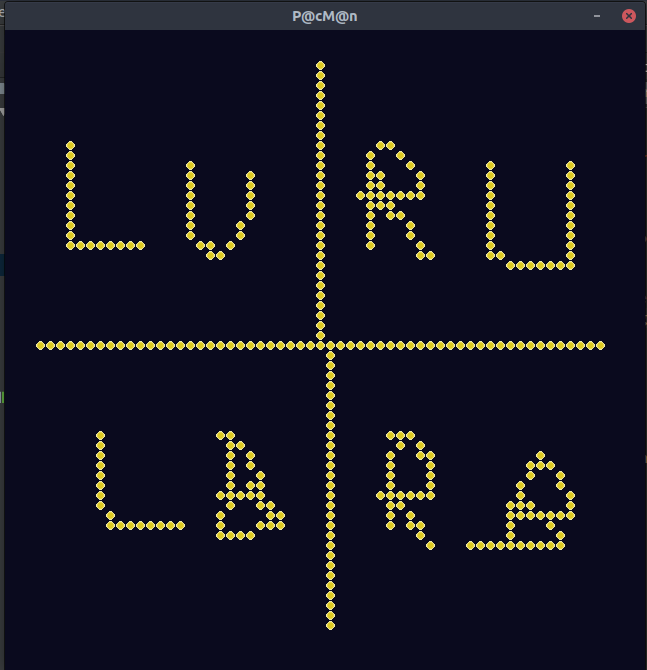
\includegraphics[width=350pt]{images/aligning-level}\\
					\caption{First tests of interpretation of level files. Note that coins are formed into letters LU, RU, LB, RB as in words Left, Right, Upper, Bottom to load the tiles in the right orientation. Old 64x64 grid is used.}
				\end{img}
				These tables are then interpreted for program to know where to place which sprites, therefore the following algorithm is used:\\
				\begin{lstlisting} [language=Python]
if level[column][row] = wall
	spawn wall at location column, row
elif level[column][row] = player
	spawn player at location column, row
elif level[column][row] = coin
	spawn coin at location column, row
elif level[column][row] = ghost
	gtype = check ghost color
	spawn ghost of color gtype at location column, row
elif level[column][row] = heart
	spawn heart at location column, row
				\end{lstlisting}
			\dsubsection{Designing the levels}
				Process of level design is quite easy and only limitation one needs to remember is that all coin - having tiles must be accessible by a player - not surrounded by a wall. The rest is just a subjective approach to the difficulty. As not all ghosts have to be used, the first few levels have one or two ghosts at most, making them easier. Through alpha testing I have noticed that long passages are traps, as one ghost may approach player from one side and other from the other and there is nowhere to hide. Also it's easier for ghosts to navigate through complex maze and these might be finger-tangling even for advanced players.
				See Figure \ref{gimplevel} for a screenshot of a design process.
			\dsubsection{User-defined levels}
				As levels can be created using a very basic bitmap editing software, user might actually add their own levels. And use them instead of the built-in ones or as an addition to them.
				
				Self-adding levels instruction is available as an appendix in Section 7 \ref{new_levels_guide}.
			\dsubsection{Progressing to the next level}
				When player eats all coins, they advance to the next level, fulfilling Requirement \ref{req-level-progress} and eventually \ref{req-level-up}. At this stage a message screen (described later) appears and all level - loading procedures are called. Also counters of coins eaten and total are reset at this point.
				
				If the level completed was the last level, a congratulations screen is displayed and the game eventually quits.
				
				See Section \ref{typesofscreens} for reference on messages signaling level change and completing the game.
		\section{Gameplay scheme}
			The game works on a concept of a loop, that (when run on a sufficiently fast machine) executes 60 times per second. During that time multiple  conditions are checked and different procedures are called.
			\dsubsection{Introduction to the concept of time segments}
				\label{timesegments}
				\begin{img}
					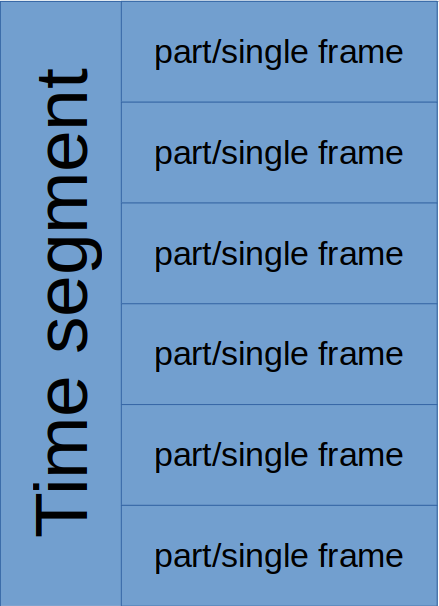
\includegraphics[width=180pt]{images/segment-part-relation}\\
					\caption{Scheme depicting relation between a time segment and parts}
					\label{segment-part-relation}
				\end{img}
				It's actually not required to compute some values every each of these 60 loop repetitions per second. An example - ghost moves $\dfrac{1}{10}^{\text{th}}$ of a tile in that time, it still can't turn so its path to the unchanged player location will remain the same. That's why I have introduced "Time segments". These are discrete representations of time period which is required for a ghost or a player to move a length of one tile. As ghost are slower, they have 5 of these in a second and player has 6. 
				\label{part_definition}
				
				Whilst processing single frames is still needed, these were called parts, whilst introducing 'part' variable determining which part of time segment is currently executed. See Figure \ref{segment-part-relation} for reference.
			\dsubsection{Player movement}
				Every player's time segment the following code is called:
				\begin{lstlisting} [language=Python]
# ----- checking pressed keys -----
keys = pygame.key.get_pressed()
# ----- wall collision check -----
surroundings = walltypecheck(player.location)
				\end{lstlisting}
				It's worth noting that I have reused walltypecheck to look for surroundings of the player for walls. See section \ref{walltypecheck} for reference on how this algorithm works.
				
				Then check is performed whether player's move is legit (wall does not obstruct it).
				\begin{lstlisting}[language=Python]
if left key pressed and tile to the left is not a wall:
	player.move('left', player_part)
elif right key pressed and tile to the right is not a wall:
	player.move('right', player_part)
elif up key pressed and tile above is not a wall:
	player.move('up', player_part)
elif down key pressed and tile below is not a wall:
	player.move('down', player_part)
				\end{lstlisting}
				Please note usage of the player\_part variable. It is the value of frames that have passed since last player segment begun (as described in Section \ref{timesegments}). It's useful to determine whether a new time segment is to be started and for player's moving routine to know at which part of tile it should position player's sprite inducing a fluency of movement.
				\begin{img}
					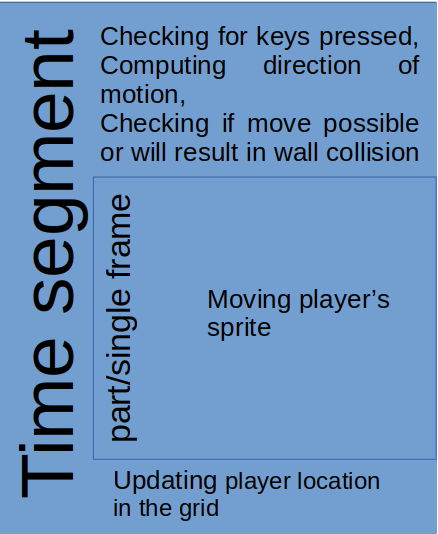
\includegraphics[width=180pt]{images/movement-diagram}\\
					\caption{Diagram showing how tasks are executed either once per time segment or once per part}
					\label{player-TS}
				\end{img}
			\dsubsection{Ghost movement}
				\label{ghost-movement}
				Ghost movement is a far more complex algorithm than player's movement though it uses same concept of time segments.
				
				As mentioned in Requirement \ref{req-smarter-ghosts}, I wanted the ghosts to be more intelligent than the originals. I have read (Reference \ref{stronaopacmanie}) that the original algorithm is really primitive. It checks from which of surrounding tiles ghost will be straight-line closest to the player and moves there.
				\subsubsection{The graph}
					First idea of mine was to make the ghost actually pick the shortest path to the player. This would both fulfill Requirements \ref{req-ghost-movement} and \ref{req-smarter-ghosts} That would have to involve implementation of a graph and a pathfinding algorithm.
					
					As I already had my level-keeping structure in place I have decided to use a similar one to store my graph. It is represented as a list of lists of lists of location tuples. It looks confusing so...\\
					A list (index i) of lists (index j) is used so that all nodes accessible from node of location (i, j) can be stored. Then that next list stores tuples (x, y) of locations accessible from that node.
					Object is named 'thegraph' throughout the program (as it is the only graph implementation in it). Note that it is a global object.
					
					It's obviously individual for each level and is built every time a level is loaded. Through the following routine:
					\begin{lstlisting}[language=Python]
def graphbuilder():
	global level, thegraph
	thegraph = [[[] for i in range(32)] for j in range(32)]
	for i in range(32):
		for j in range(32):
			if level[i][j] != wall:
				location = [i, j]
				if location[0] != 0:
					if level[location[0] - 1][location[1]] != 	wall:
						thegraph[location[0]][location[1]] += [[location[0] - 1, location[1]]]
				if location[0] != 31:
					if level[location[0] + 1][location[1]] != wall:
						thegraph[location[0]][location[1]] += [[location[0] + 1, location[1]]]
				if location[1] != 0:
					if level[location[0]][location[1] - 1] != wall:
						thegraph[location[0]][location[1]] += [[location[0], location[1] - 1]]
				if location[1] != 31:
					if level[location[0]][location[1] + 1] != wall:
						thegraph[location[0]][location[1]] += [[location[0], location[1] + 1]]
					\end{lstlisting}
					Notably, this algorithm neither adds wall as neighbors of other tiles, nor produces neighbors for wall tiles. This successfully prevents ghosts from moving onto wall tiles, therefore fulfilling Requirement \ref{req-walls-not-passable}. 
				\subsubsection{Pathfinding}
					This part I found actually the hardest. All my previous experience with graphs and pathfinding was actually from old times when my favorite language was C++. Apparently when I switched to Python, my rusty knowledge on the topic had to be refreshed. My first approach (a stupid one) was to use DFS search to check all possible paths and decide which one to use.
					\begin{img}
						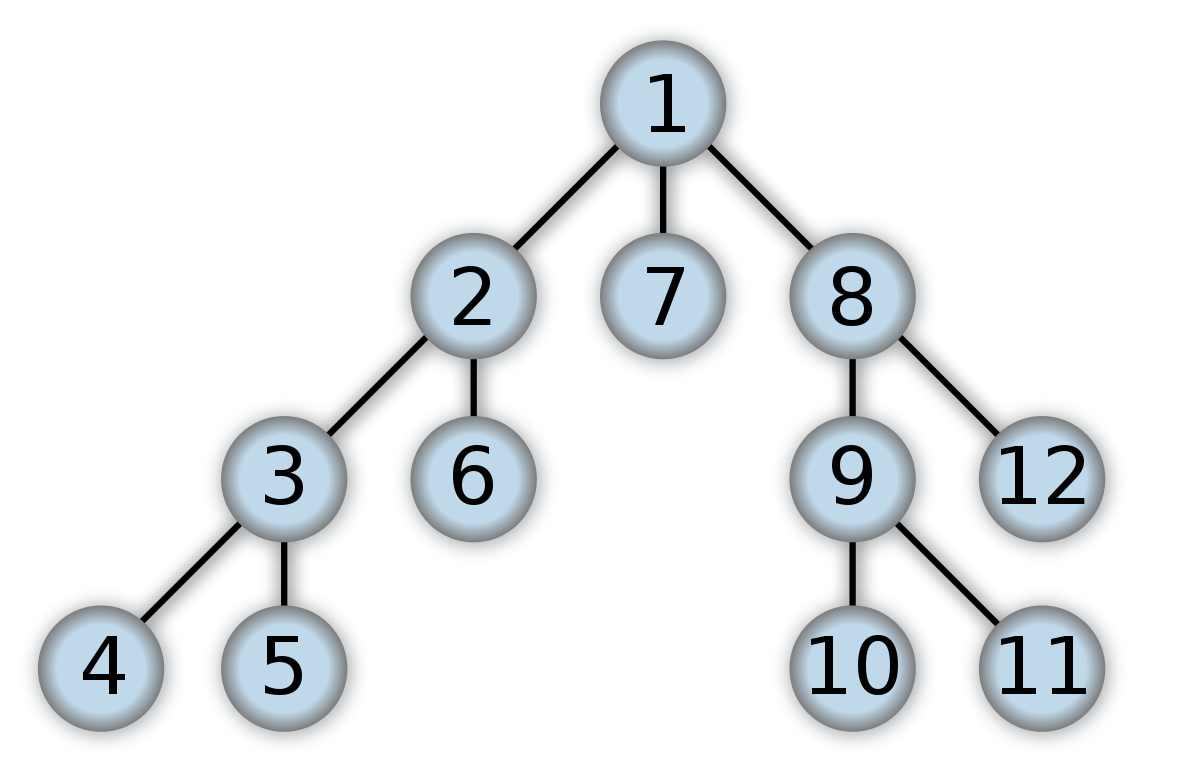
\includegraphics[width=350pt]{images/dfs-diagram}\\
						\caption{Diagram showing order of nodes visits starting from node 1 using DFS algorithm Source: wikipedia.org}
						\label{DFSalg}
					\end{img}
					It was a rather simple recursion.
					\begin{lstlisting} [language=Python]
def findpath(start, end, path):
	append start to path
	if start == end:
		return path
	else:
		for neighbour in neighbours(start): # neighbours easily obtained from thegraph
			findpath(neighbour, end, path)
					\end{lstlisting}
					That was stupid and very slow, as I have noticed that my graph is not actually a tree and paths may have cycles, this process never actually worked.
					
					And then I realized that a more appropriate solution was to use BFS and implement whether a new node was actually visited before.
					
					\begin{img}
						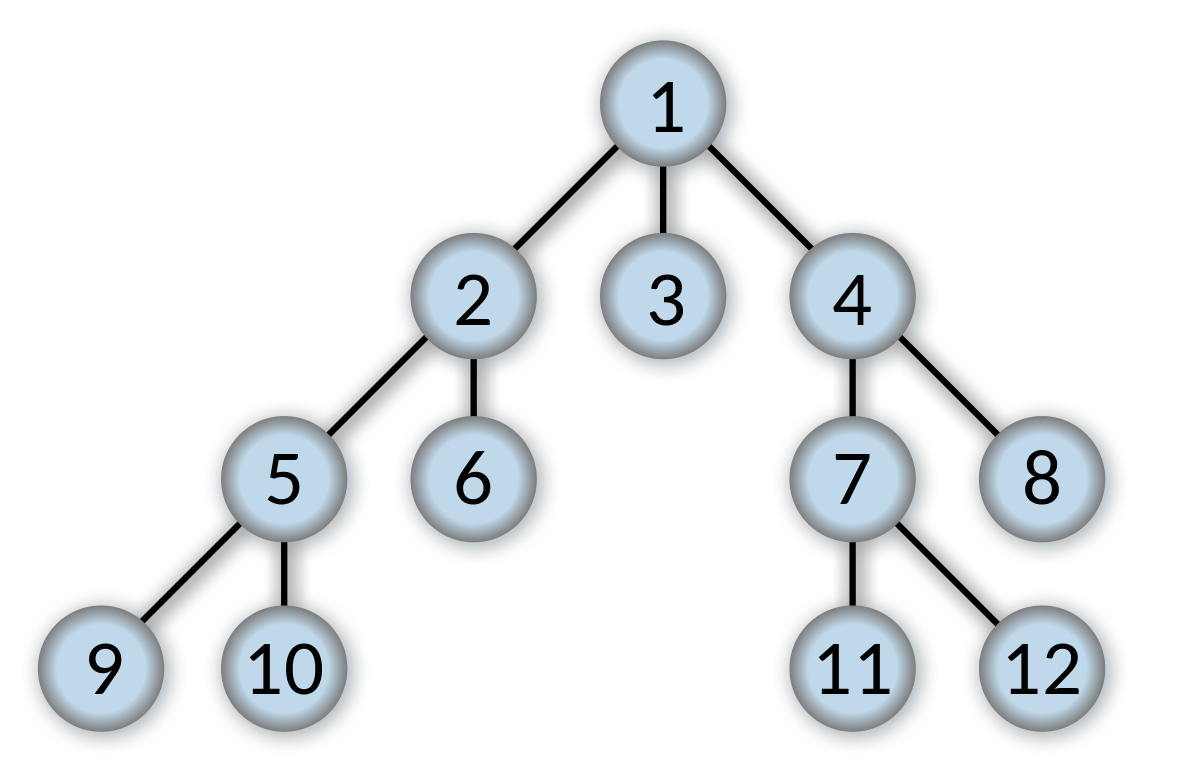
\includegraphics[width=350pt]{images/bfs-diagram}\\
						\caption{Diagram showing order of nodes visits starting from node 1 using BFS algorithm Source: wikipedia.org}
					\end{img}
					
					I also dropped recursion as advised by online forums... Maybe recursion is a way in C++ but in Python it apparently is really slow. Also my own testing of recursive approach sometimes led to stack overflows, which disqualified this method completely.
					
					A queue of nodes to visit was implemented and new algorithm came to life. It was fast but its output of a complete path to player was actually an overkill - why would I need it if it will become obsolete in the next time segment when player location changes?
					
					The next iteration actually begins BFSing from the player, until it finds any of the tiles surrounding the ghost. It then returns location of such tile - next tile ghost has to move to.
					
					\begin{lstlisting}[language=Python]
def find_next_move(start, end, forbidden):
	visited = []
	queue = []
	neighbours = thegraph[start[0]][start[1]].copy()
	queue.append([end[0], end[1]])
	visited.append(end)
	for point in queue:
		if point not in visited:
			visited.append(point)
		if point in neighbours:
			return point
		for node in thegraph[point[0]][point[1]]:
			if node not in visited:
				queue.append(node)
					\end{lstlisting}
					
					As this approach worked, I was satisfied with its speed and overall performance. Then in alpha testing I found a strange occurrence I haven't noticed in the original PacMan - ghosts could reverse.
					
					I didn't like it, so the algorithm had to exclude ghost's previous location from its neighboring tiles. The next version looked like this:
					\begin{lstlisting}[language=Python]
def find_next_move(start, end, forbidden):
    visited = []
    queue = []
    neighbours = thegraph[start[0]][start[1]].copy()
    neighbours.remove([forbidden[0], forbidden[1]])
    queue.append([end[0], end[1]])
    visited.append(end)
    for point in queue:
        if point not in visited:
            visited.append(point)
        if point in neighbours:
            return point
    for node in thegraph[point[0]][point[1]]:
        if node not in visited and node != [forbidden[0], forbidden[1]]:
    queue.append(node)
					\end{lstlisting}
				\subsubsection{Differences between ghosts}
					\label{hunting}
					As I have generated some levels and started testing, I found out that if two ghost share location, they effectively become one as their optimal paths will be the same and they will always move the same way. That of course wasn't the effect I wanted, I had to figure out how to make the ghosts behave different. But how to make ghosts both smart and not going straight for the player? Internet for the win, meme pages came with help.
					\begin{img}
						
\includegraphics[width=350pt]{images/trap}\\
						\caption{Popular meme. Source: pinterest.com}
						\label{trap}
					\end{img}
					Now enlightened by a piece of digital artwork originating from Star Wars (see Figure \ref{trap}), I decided that my ghosts have to behave like they were to surround the player. How to achieve such effect? I turned to the original PacMan solution - not moving to the exact tile the player occupies. A decision was made to leave the red ghost originally smart while blue and green ghosts were to move to tiles shifted by (-2, -2) and (2, 2) vectors from the player. The result was amazing, ghosts seemed to move separately while away from the player, when they approach it, I had a sense that this is not what I programmed, \textbf{They hunt in a pack!} I had an authentic experience of ghosts setting a trap, green and blue were blocking my exit routes, when red went straight for me. I put a big green tick mark by the Requirement \ref{req-ghost-differences}.
					
					But it sometimes crashed, I wondered what was the case and then I found out that the ghosts were actually trying to go to a tile, which is either a wall (inaccessible) or outside the board (object level was referenced with an invalid index, either negative or exceeding it's length). I had to write a piece of algorithm to look for a nearest tile that is actually not wall.
					
					\begin{lstlisting} [language=Python]
def find_nearest_not_wall(point):
    if point[0] > 31:
        point[0] = 31
    if point[0] < 0:
        point[0] = 0
    if point[1] > 31:
        point[1] = 31
    if point[1] < 0:
        point[1] = 0
    radius = 1
    if level[point[0]][point[1]] != wall:
        return point
    while True:
        for i in range(point[0]-radius, point[0]+radius):
            for j in range(point[1]-radius, point[1]+radius):
                try:
                    if level[i][j] != wall:
                        return [i, j]
                except IndexError:
                    pass
        radius += 1
					\end{lstlisting}
					It first moves the point to the nearest one on the board (lines 2 to 9). Then it checks whether such point is a wall, if not, returns it (lines 11 and 12). If it was a wall it starts searching surroundings of such point in a fixed radius, starting from 1. First point it finds not to be wall is then returned.
					
					Later it had to be implemented in the pathfinding algorithm, which now looks like this:
					\begin{lstlisting} [language=Python]
def find_next_move(start, end, forbidden):
    visited = []
    queue = []
    end = find_nearest_not_wall(end)
    neighbours = thegraph[start[0]][start[1]].copy()
    neighbours.remove([forbidden[0], forbidden[1]])
    queue.append([end[0], end[1]])
    visited.append(end)
    for point in queue:
        if point not in visited:
            visited.append(point)
        if point in neighbours:
            return point
    for node in thegraph[point[0]][point[1]]:
        if node not in visited and node != [forbidden[0], forbidden[1]]:
    queue.append(node)
					\end{lstlisting}
					Note line 4. where final point is substituted with a one closest to it being actually accessible.
					
				\subsubsection{Calling pathfinding algorithm}
					Now, every ghosts' time segment (note that all ghosts share a single time segment), a new destination tile is calculated for each ghost and pathfinding is called to determine which tile should the ghost move to throughout the time segment.
					\begin{lstlisting} [language=Python]
for ghost in ghosts_list:
    if ghost.color == 'red':
        ghost.nexttile = find_next_move(ghost.location, player.location, ghost.previouslocation)
    elif ghost.color == 'blue':
        ghost.nexttile = find_next_move(ghost.location,
                                        [player.location[0] + 2,
                                         player.location[1] + 2],
                                        ghost.previouslocation)
    elif ghost.color == 'green':
        ghost.nexttile = find_next_move(ghost.location,
                                        [player.location[0] - 2,
                                         player.location[1] - 2],
                                        ghost.previouslocation)
					\end{lstlisting}
					Note how find\_next\_move function takes arguments of:
					\begin{enumerate}
						\item
							Ghost location
						\item
							Target location
						\item
							Previous ghost location - forbidden tile as ghosts can't reverse.
					\end{enumerate}
				\subsubsection{Ghosts speed}
					As I had ghosts chasing me, I have figured out that the player actually can't outrun them. And every suboptimal move of the player led to red ghost getting closer and closer. I had the smartest ghost possible, but it had an advantage of having no means of being killed. It was a too powerful opponent. I didn't want to add power-ups for the player to either become faster or to be able to frighten/kill the ghosts. Instead, as derived from the Interview (see Section \ref{interview}), I decided to make the ghosts move at $\dfrac{5}{6}^{\text{th}}$ of the player's speed. I found the gameplay to be quite optimal and actually started playing the game which at this stage was only running from the ghost. But with a stopwatch I was challenged to keep my distance from them for quite a long time. I finally knew that this is what I was aiming for.
			\dsubsection{Handling movement animation}
				This section is common for both ghosts and a player as it actually derives from the same code. As mentioned in Section \ref{part_definition}, the part part is a smaller piece of time segment. During a single part no routes are computed for ghosts, they only move from one tile to another, being able to actually be rendered in between these tiles to make the Movables (ghosts + player sprites) move fluently.
				\begin{lstlisting} [language=Python]
def move(direction,
				segmentsize,
				part):
	# handling multiple direction formats
    if direction == 'up' or direction == (0, 1):
        speed = (0, -1)
    elif direction == 'down'or direction == (0, -1):
        speed = (0, 1)
    elif direction == 'left' or direction == (-1, 0):
        speed = (-1, 0)
    elif direction == 'right' or direction == (1, 0):
        speed = (1, 0)
    part2 = (part+1) / segmentsize #as parts are numbered from 0
    #rect parameters of a Movable as implemented in pygame
    rect.x, rect.y = (location[0] + speed[0] * part2) * tile_width,
                     (location[1] + speed[1] * part2) * tile_width
    if part == segmentsize - 1:
    #if movement came to the end update location
        location = location[0] + speed[0],
                   location[1] + speed[1]
				\end{lstlisting}
				\begin{enumerate}
					\item
						Speed vector is derived from parameter 'direction' (lines 4-12)
					\item
						part2 is calculated - fraction of progress of the movement to be completed in this part (line 13)\
					\item
						Movable sprite is moved to new position (lines 14-16)
					\item
						If the actual movement came to an end and a Movable is in a center of a next tile location is updated (lines 17-20)
				\end{enumerate}
			\begin{img}
				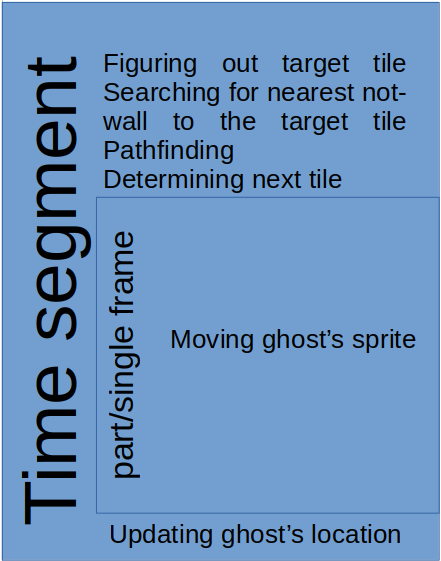
\includegraphics[width=180pt]{images/ghost-time-segment}\\
				\caption{Diagram showing how tasks are executed either once per time segment or once per part (for a ghost) \newline See Figure \ref{player-TS} for the same for player.}
			\end{img}
			\dsubsection{Eating}
				Eating of both coins and hearts (Eatables) was easy to implement in terms of detection, but I had to look up how to destroy eaten sprites in the pygame documentation. I found that Sprites may be killed, which seemed to be an optimal solution to that problem. Therefore every player's time segment the following routine is called.
				\begin{lstlisting} [language=python]
for eatable in eatables:
	if eatable.location == player.location:
		if eatable == heart:
			lifes += 1
		if eatable == coin:
		 coins_eaten += 1
		eatable.kill()
				\end{lstlisting}
				For every eatable is checked for occupying the same tile as player.\\
				Then if it is a heart, player gains a life, as per Requirement \ref{req-lifes++}.\\
				if it was a coin, coins eaten counter increases, as per Requirement \ref{req-point++}.\\
				Eatable sprite is killed. This fulfills Requirement \ref{req-coins-disappearing}.
			\dsubsection{Getting killed}
				Killing a player is fairly similar to eating... It's just checking for collision with a Ghost instead of an Eatable. It's also called every player's time segment \textbf{or} every ghosts' time segment.
				Following routine is then called:
				\begin{lstlisting} [language=python]
for ghost in ghosts:
	if ghost.location == player.location:
		lives -= 1
		if lives == 0:
			pull Game Over screen
		Respawn every Movable
		Reset parts
		Wait 5s
		Continue game
				\end{lstlisting}
				For every ghost a collision with player is checked, if such is detected, process of dying begins.\\
				Life is subtracted from lives counter. (As per Requirement \ref{req-life-loss})\\
				If player has no more lives the game ends. (Requirement \ref{req-game-over})\\
				If there are more lives, all movables return to their original position (described in Section \ref{respawning})
				and part counters are reset.\\
				Game waits 5 seconds to let the user cope with the loss, and continues.
			\dsubsection{Respawning after a loss of life}
				\label{respawning}
				This is a relatively simple process of putting all Movables to their initial position and making them not preserve their speed. It can be easily described with a following code:
				\begin{lstlisting} [language=Python]
for Movable in Movables:
    Movable.location = Movable.initiallocation
    Movable.speed = (0, 0)
				\end{lstlisting}
				This process is often referred to as reseting within this document as well as in the corresponding code. This function fulfills the Requirement \ref{req-reset}.
		\section{Types of message screens}
			\label{typesofscreens}
			Messages present throughout the game are displayed in a way that prevents any game event, from occurring unless the message is dismissed by pressing space.
			
			It's done through occupying the main thread with checking for spacebar being pressed.
			\begin{img}
				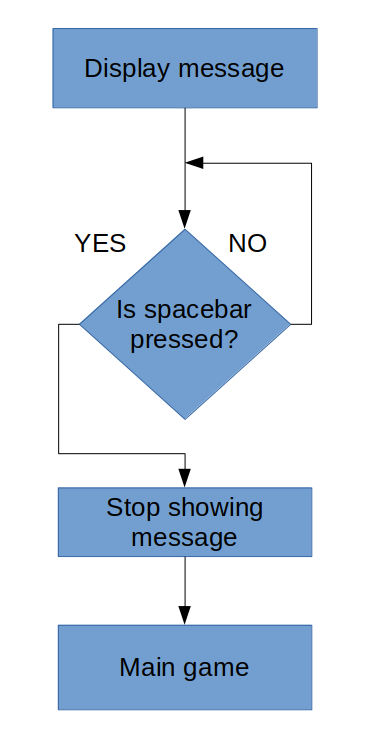
\includegraphics[width=100pt]{images/message-dismiss}\\
				\caption{Diagram showing how game is halted until message is dismissed using spacebar}
			\end{img}
			\begin{img}
				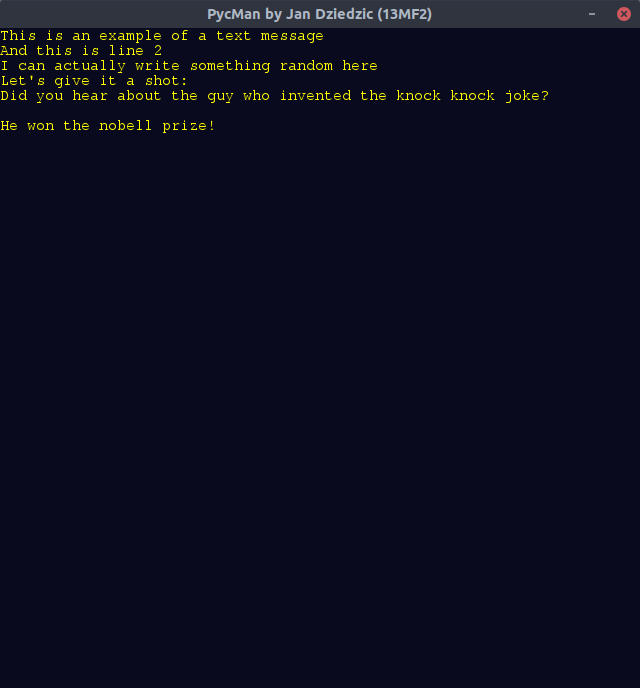
\includegraphics[width=250pt]{images/message-example-joke}\\
				\caption{Exemplar of the message screen appearing in a window rendered in Ubuntu Gnome graphical environment}
			\end{img}
			\dsubsection{Tutorial}
				\begin{img}
					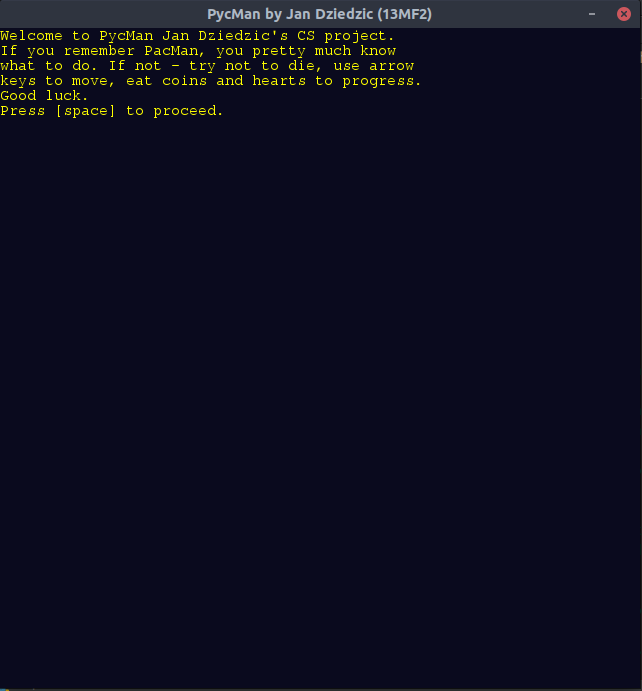
\includegraphics[width=300pt]{images/tutorial.png}\\
					\caption{Message displayed after starting the game. Shown in a game window rendered in the Ubuntu Gnome graphical environment.}
				\end{img}
			\dsubsection{Loss of life}
				\begin{img}
					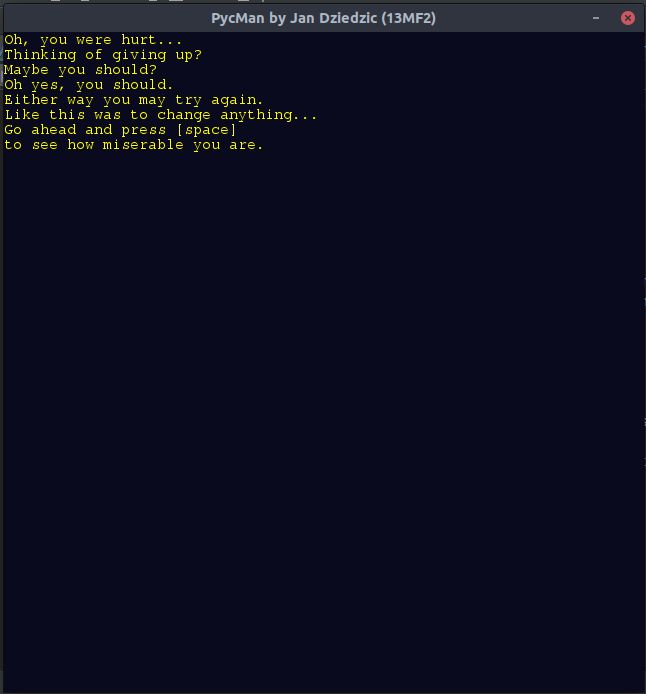
\includegraphics[width=300pt]{images/loss_of_life_msg.png}\\
					\caption{Message displayed after losing a life. Shown in a game window rendered in the Ubuntu Gnome graphical environment.}
				\end{img}
			\dsubsection{Completing a level}
				\begin{img}
						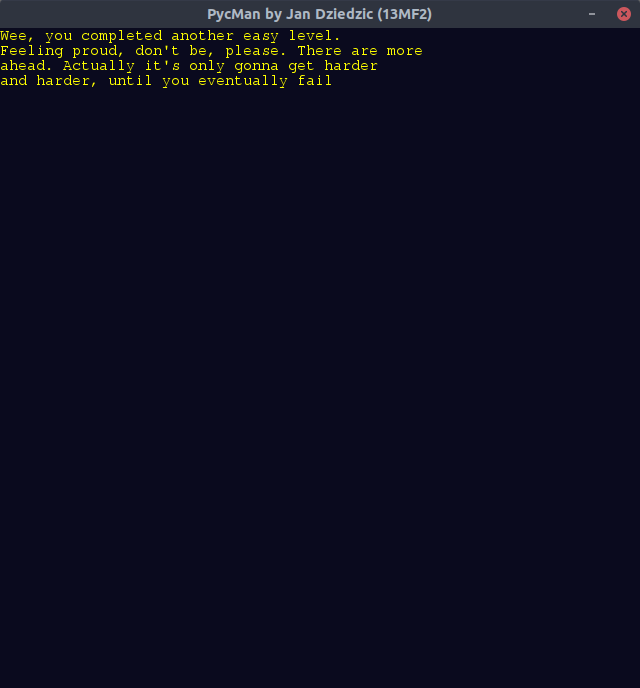
\includegraphics[width=300pt]{images/level-complete.png}\\
						\caption{Message displayed after completing a level. Shown in a game window rendered in the Ubuntu Gnome graphical environment.}
				\end{img}
			\dsubsection{Loosing the game}
				\begin{img}
					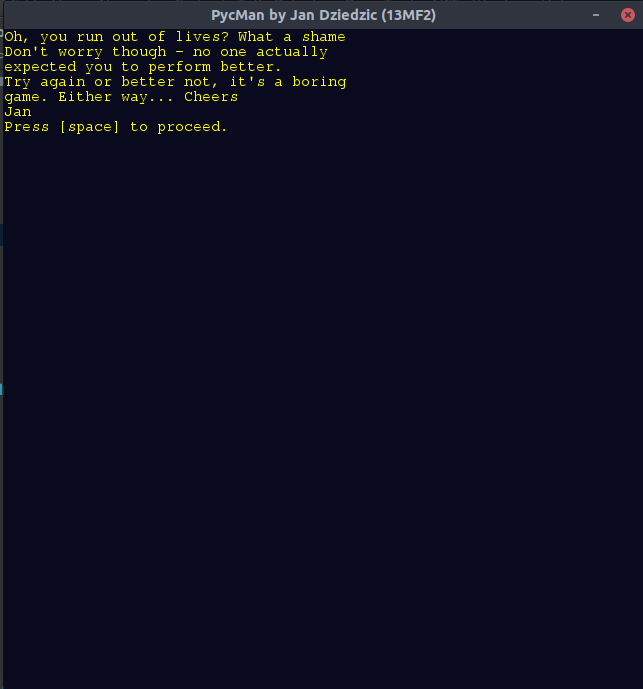
\includegraphics[width=300pt]{images/game_over_msg.png}\\
					\caption{Message displayed upon losing the game. Shown in a game window rendered in the Ubuntu Gnome graphical environment.}
				\end{img}
			\dsubsection{Completing the entire game}
				\begin{img}
					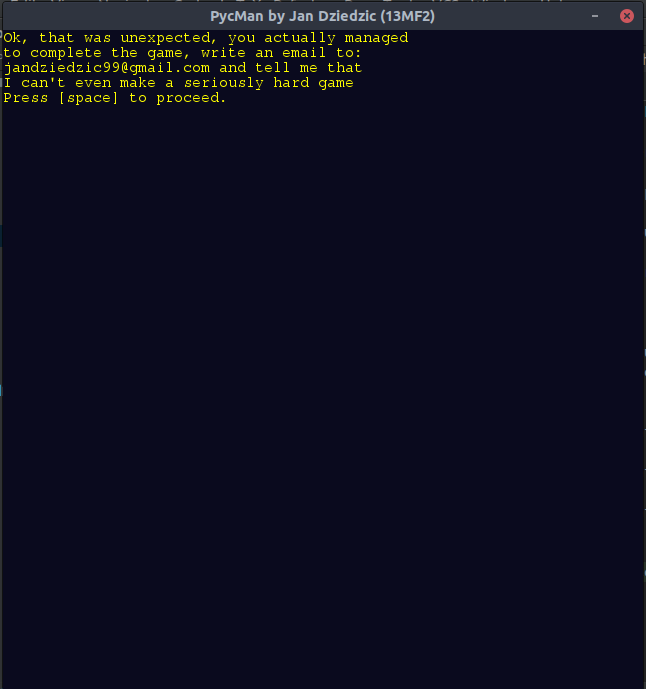
\includegraphics[width=300pt]{images/real_congrats_msg.png}\\
					\caption{Message displayed after completing the game. Shown in a game window rendered in the Ubuntu Gnome graphical environment.}
				\end{img}
		\section{Testing}
			I have decided to use three stages of testing, namely zero, alpha ($\alpha$) and beta ($\beta$).
			\dsubsection{zero-testing}
				This stage was introduced while testing single functions and procedures implemented through the game during the development process. It consisted of mostly running code as-is while writing it using PyCharm. Sometimes I haven't even use debugger in favor of print function to enlist values of variables. This phase commenced until all modules of the game were actually prepared, despite being containing minor bugs that didn't immediately throw an error. At the end of this stage, the game was playable. 
			\dsubsection{$\alpha$-testing}
				This was the stage of extensively playing the game to see whether all functions appear to be working correctly. Note the use of word 'appear' - code wasn't actually read at this stage in look for bugs, only user experience was assessed. I have tried different approaches at playing, to make the game algorithms experience different user input. From staying perfectly still to going straight for a ghost, I have played the game checking the following:
				\begin{enumerate}
					\item
						Getting killed by the ghost approaching from different angles.
					\item
						Eating Eatables from different angles.
					\item
						Trying to pass through numerous walls.
					\item
						Moving the player in different directions repeatedly to check if ghosts get confused and the gameplay remains fluent.
					\item
						Manual counting of coins eaten to see if it matches the counter value.
					\item
						Checking whether all graphics render well, by creating each wall type and each possible sprite.
					\item
						Providing program with unexpected input of unassigned keys, mouse clicks and even connecting a gamepad.
				\end{enumerate}
			\dsubsection{$\beta$-testing}
				This was a stage of testing, during which all major bugs were resolved and the assessment was focused on user experience. Following procedures were performed:
				\begin{enumerate}
					\item
						Smoothness of animations was checked on different computers, running different OSs.
					\item
						Graphics quality was assessed by an independent body, namely my sister.
					\item
						Actual playing was performed and all levels were played. Each level was actually completed, but never in a single sitting, proving that game indeed can be completed, though it is considerably hard.
					\item
						Different players were used to test the game play.
					\item
						Quality of input controls was assessed.
				\end{enumerate}
	\chapter{Implementation}
		In this section the detailed description of how the game files were created is provided.
		\section{Programming tools}
			Whole development of the game, as mentioned in Section \ref{freeware}, was done using a Ubuntu running computer and legally obtained tools I didn't have to pay for, namely opensource, freeware or free for education software.
			\dsubsection{PyCharm}
				I used, in my opinion, a brilliant Python IDE called PyCharm. Developed by a company JetBrains and obtained under Free for Education license for the entirety of the project development. The program has a lot of useful functions, which made my work easier and admittedly contributed to me learning how to code more efficiently.
				\begin{img}
					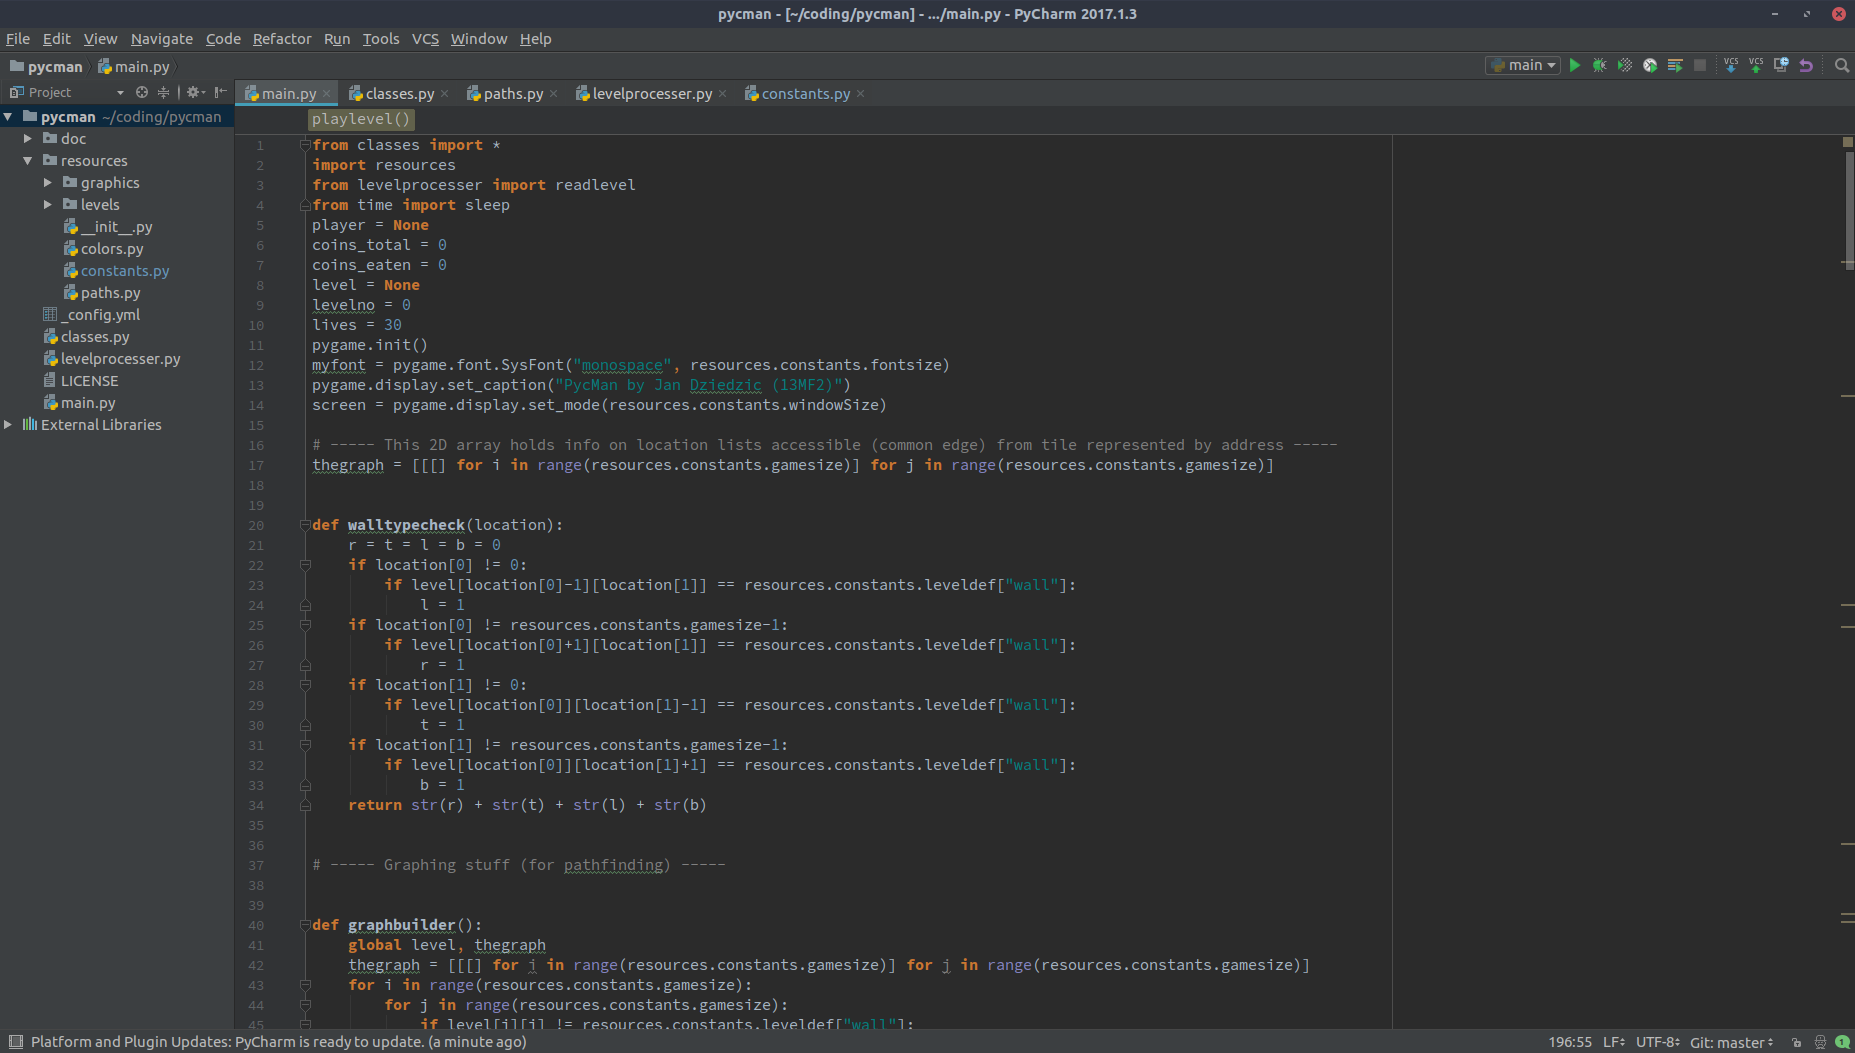
\includegraphics[width=350pt]{images/pycharm}\\
					\caption{Pycharm window rendered in Ubuntu Gnome environment with Pycman project loaded.}
				\end{img}
			\dsubsection{GIMP}
				GIMP software was used to develop graphical resources for the game as well as for this document. It's an open source community-developed tool for graphics manipulation, which sometimes is referred as the free alternative to the Adobe Photoshop, with advanced functions and ability to edit images with Alpha channel, resulting in capacity to make ghost images semitransparent. See Figure \ref{ghostimage} for reference.
			\dsubsection{Git}
				Git is a popular tool for VCS (Version Control System). My previous experience with programming and mostly teamwork made me use it as an obvious choice for keeping my project files. I used free Github for Education account and github.com servers for storing my files. Admittedly it was really useful when I had to revert some advanced changes or look up how something worked earlier, as it worked better. Basically speaking - it made mistakes less painful.
				\begin{img}
					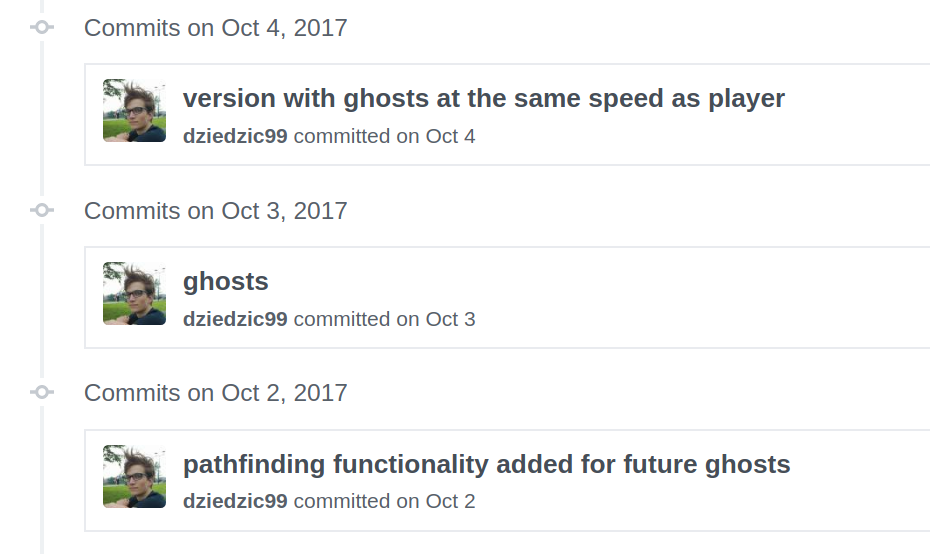
\includegraphics[width=300pt]{images/github.png}\\
					\caption{Screenshot of the lists of some of the project commits in the GitHub web interface.}
				\end{img}
			\dsubsection{TeXstudio}
				TeXstudio was used to write this document. \LaTeX with its excellent reference system as well as professional look was the most appropriate tool in my opinion.
				\begin{img}
					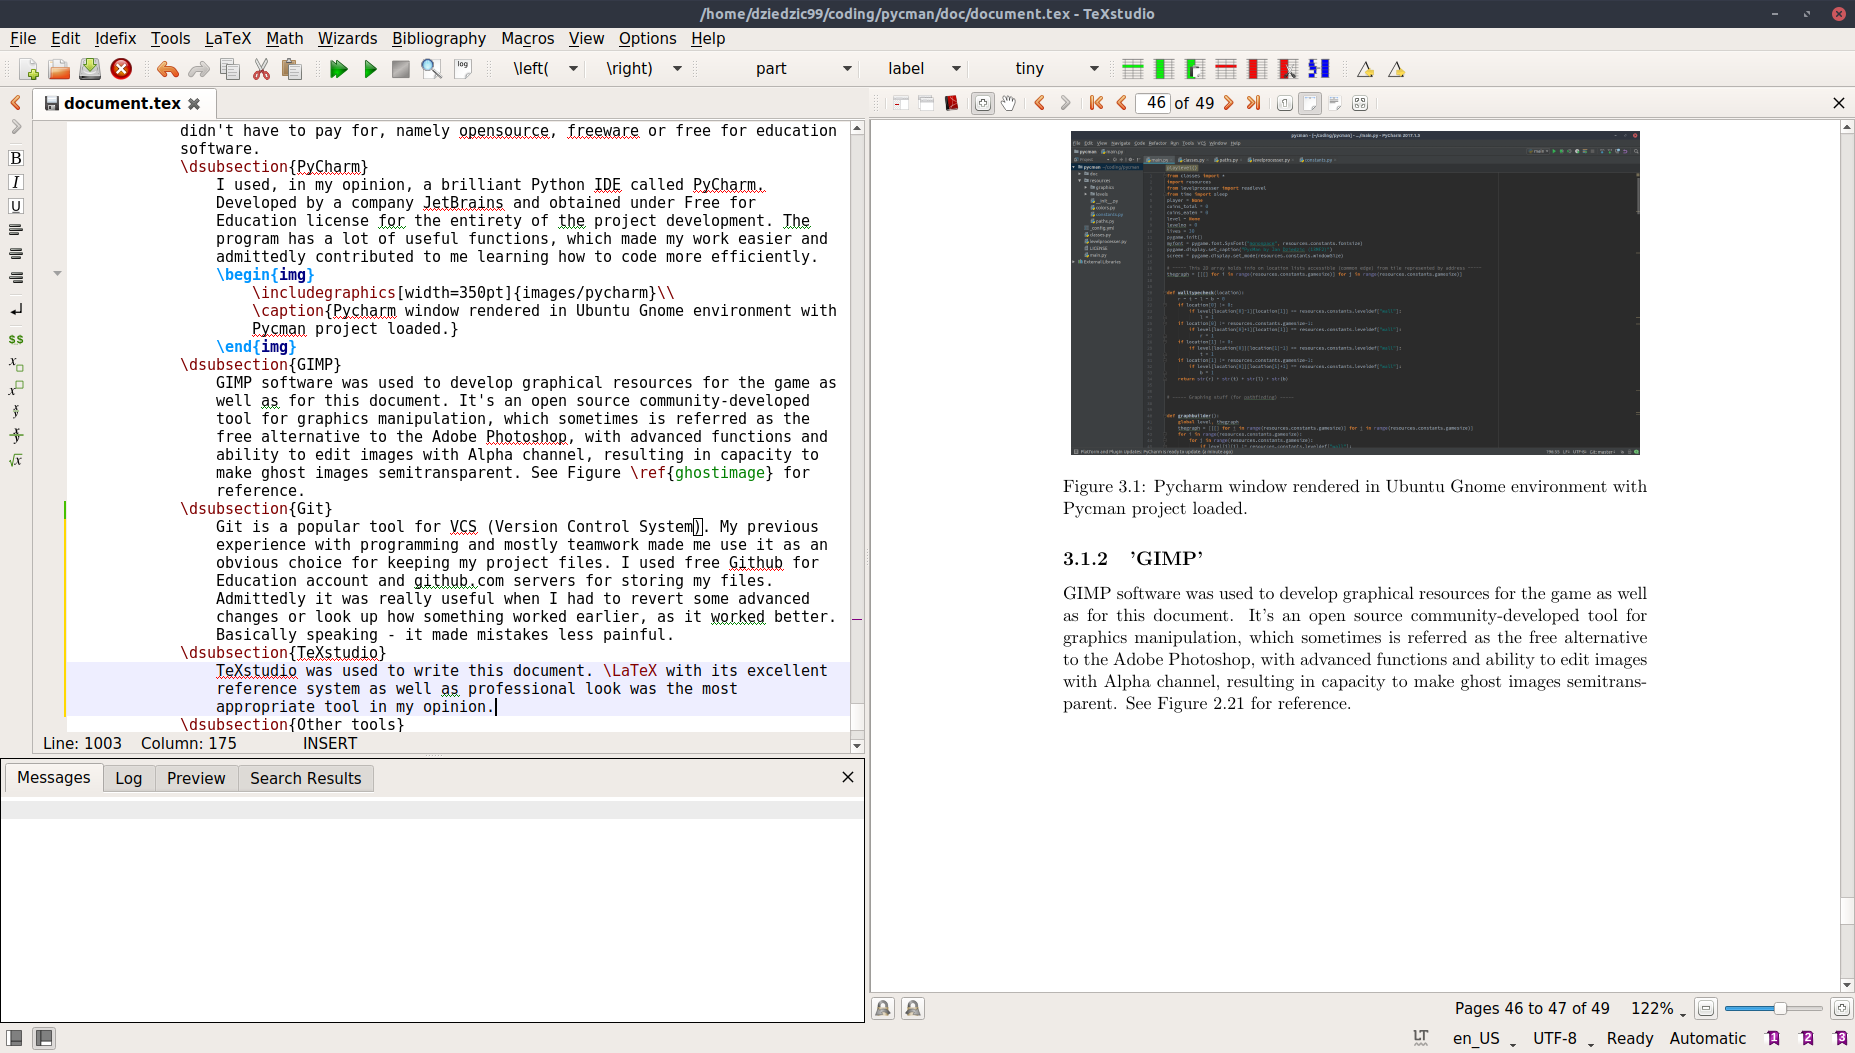
\includegraphics[width=350pt]{images/texstudio}\\
					\caption{TeXstudio window rendered in Ubuntu Gnome environment with this document loaded.}
				\end{img}
			\dsubsection{Other tools}
				Minor other programs were used for writing this documentation, mostly for obtaining screenshots and producing flowcharts.
		\section{Interpreter and its modules}
			\dsubsection{Virtual Environment}
				To keep my computer clean and my main /usr/bin Python interpreter free of heavy, not often used modules as Pygame I have decided to create a separate interpreter instance using Virtualenv tool.
			\dsubsection{Modules}
				Modules used by the game are as follows:
				\begin{itemize}
					\item Pygame - for graphics rendering and input control. Origin of the Sprite class.
					\item Pillow A.K.A. PIL - for loading level files
					\item time - origin of the function sleep for delaying certain actions.
				\end{itemize}
		\section{Project structure}
			I have decided to make the project structure as professionally organized as possible. Therefore I have divided program into resource files and Python files, keeping the first separate in a different folder. Documentation and its resources - graphics are also stored separately.
			\begin{img}
				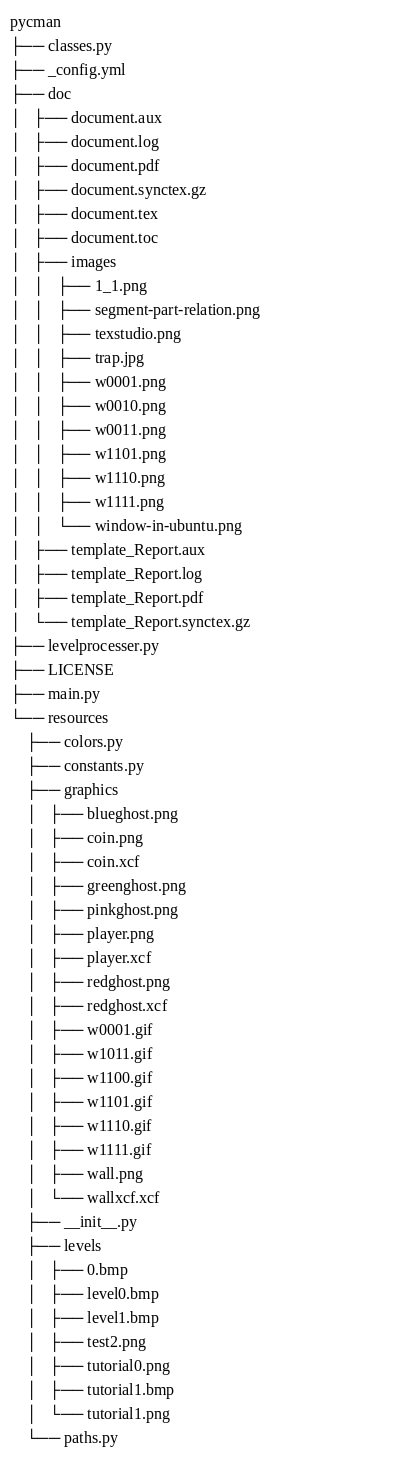
\includegraphics[width=120pt]{images/directory_structure}\\
				\caption{Abbreviated directory structure layout}
			\end{img}
			Reason for additional Python files will be provided within this Chapter.
		\section{Classes}
		\label{classes}
			\begin{img}
				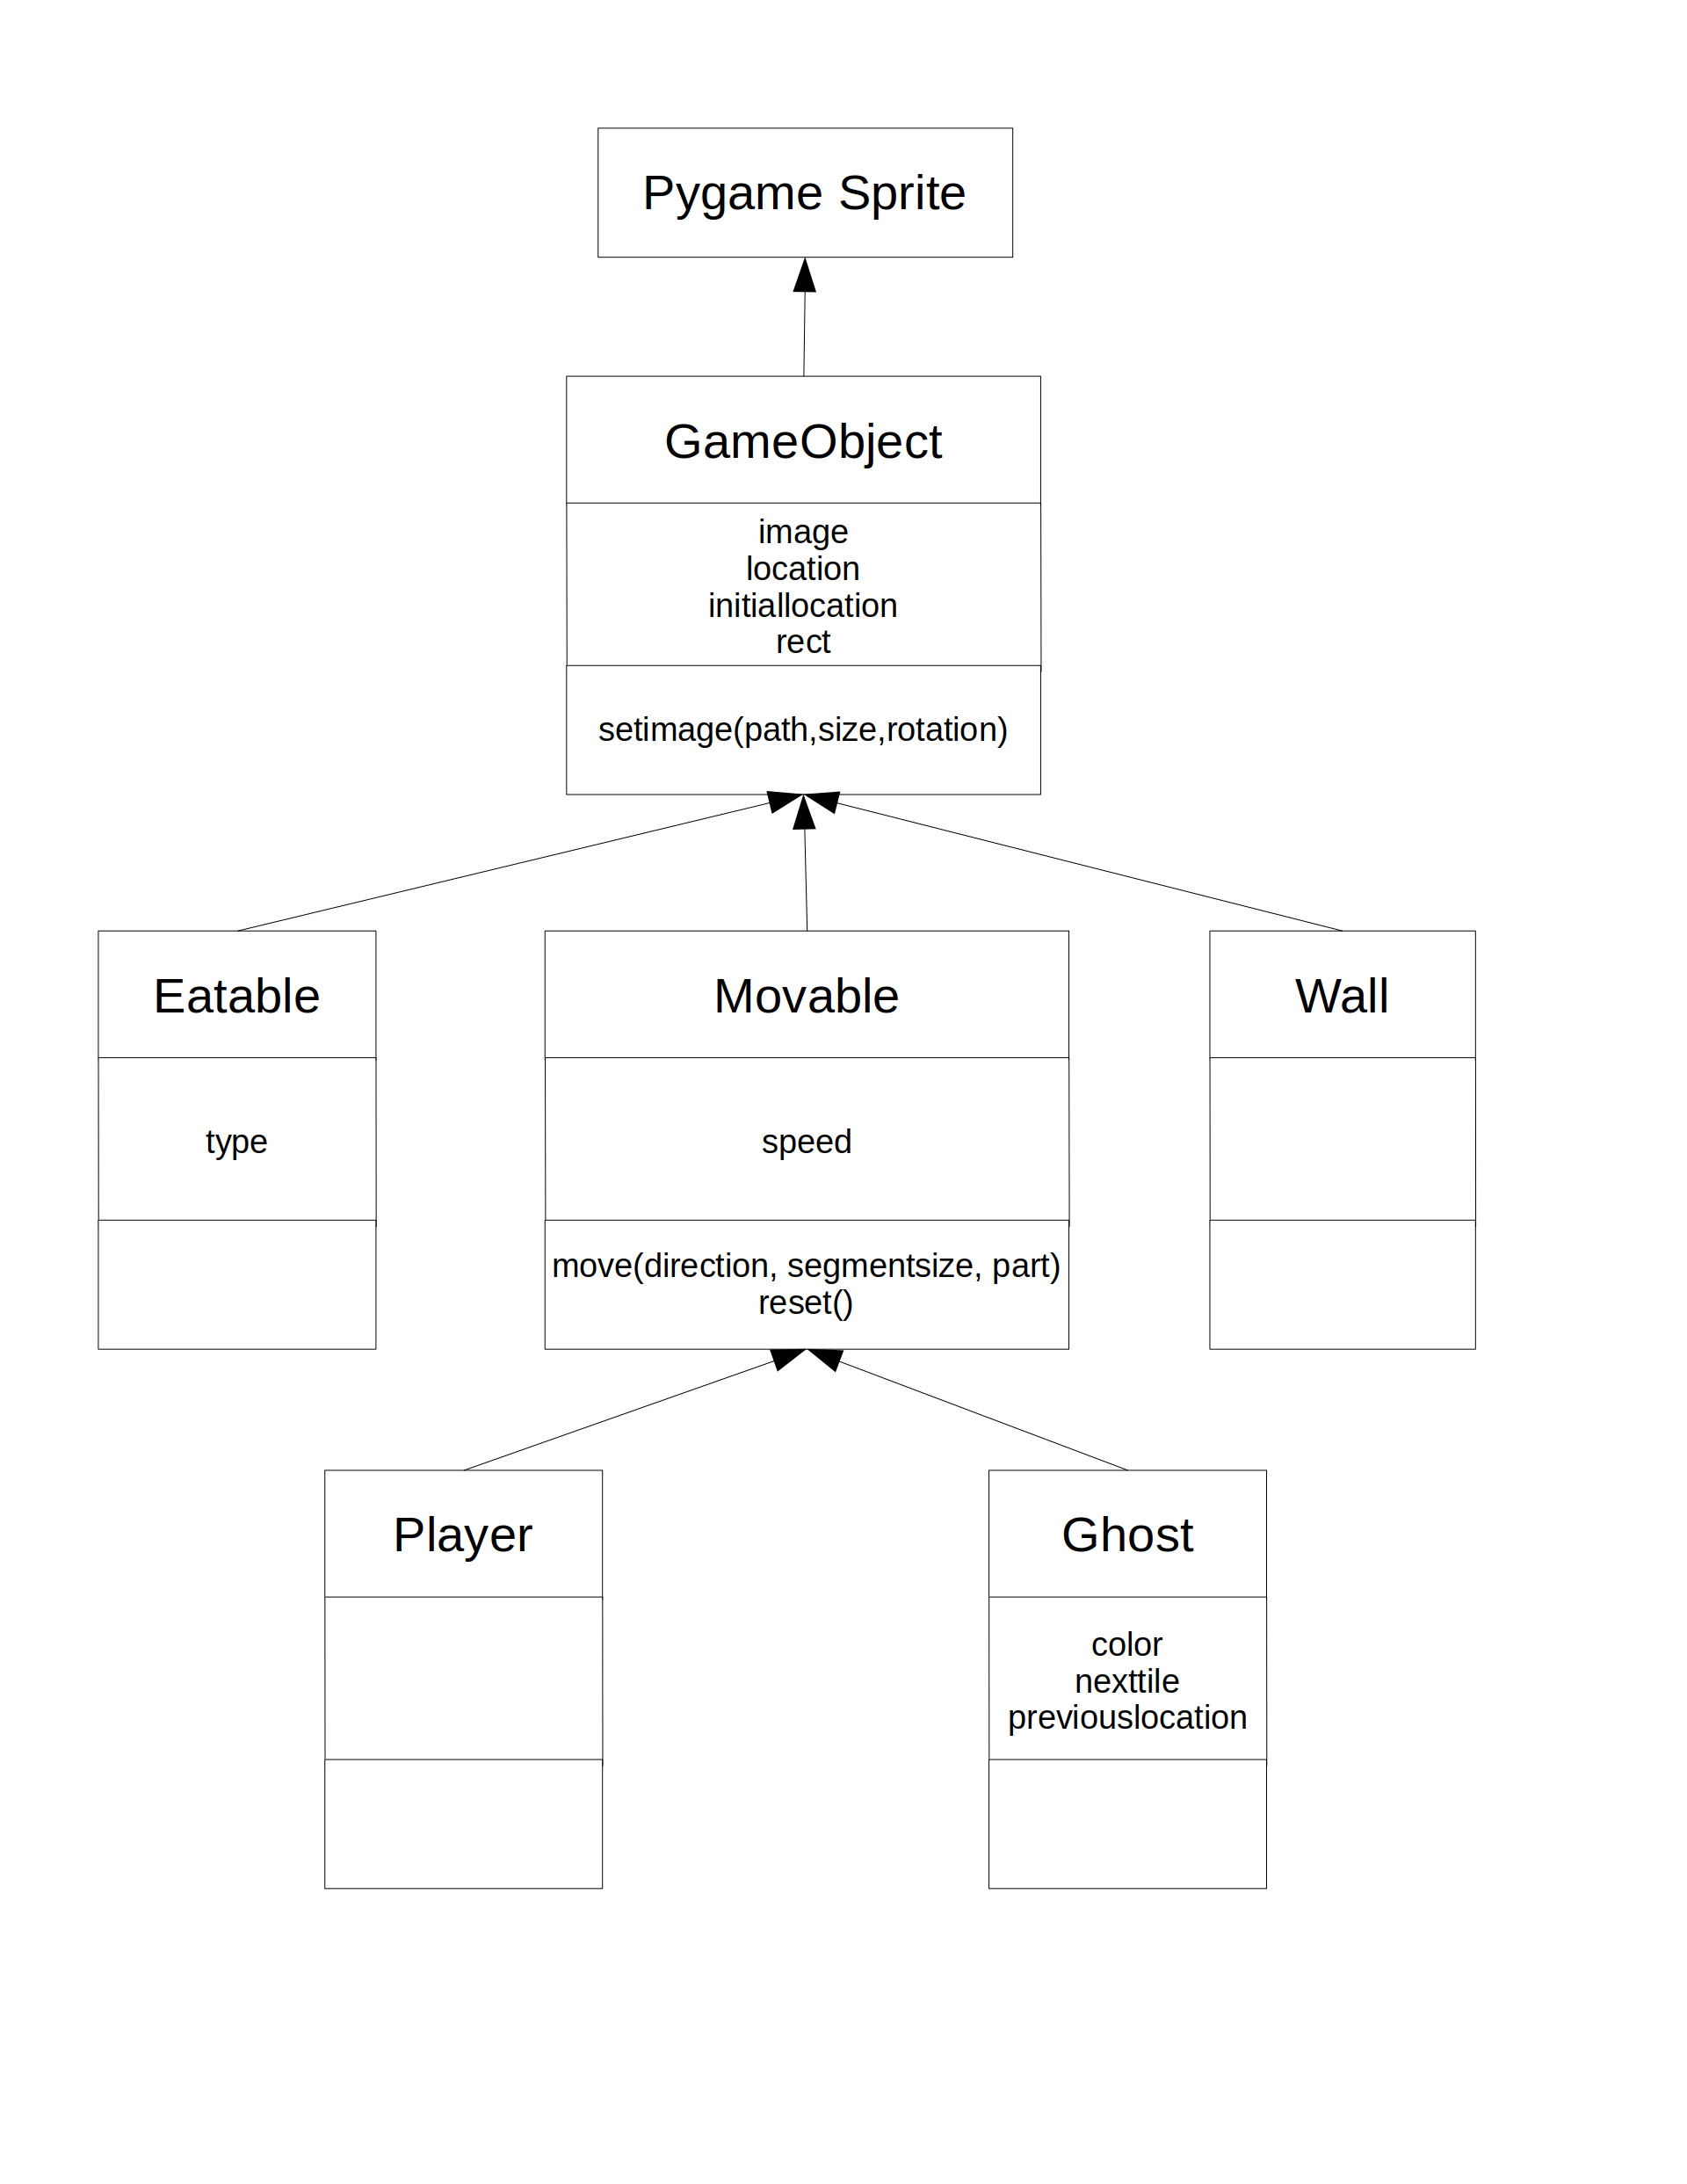
\includegraphics[width=400pt]{images/class_diagram}\\
				\caption{Project class diagram}
			\end{img}
			\dsubsection{GameObject}
				As whole game is written around pygame environment I have decided to utilize Pygame Sprite class for all objects (excluding text) rendering on the screen. To facilitate some concepts I assumed in the Design stage I had to add a GameObject class.\\
				Class code:
				\begin{lstlisting} [language=Python]
class GameObject(pygame.sprite.Sprite):
	def __init__(self, location):
		super().__init__()
		self.image = None
		self.location = location
		self.initiallocation = location
		self.rect = None

	def setimage(self, image, size=resources.constants.boxSize, rotation=0):
		self.image = pygame.image.load(resources.paths.image[image])
		self.image = pygame.transform.scale(self.image, size)
		self.image = pygame.transform.rotate(self.image, rotation)
		self.rect = self.image.get_rect()
		self.rect.x, self.rect.y = self.location[0] * resources.constants.boxSegmentSize, self.location[1] * resources.constants.boxSegmentSize
				\end{lstlisting}
				The most important part of the class is the 'location' attribute. It is an (integer, integer) tuple storing information of location of the object in a grid, as described in Section \ref{grid}. Location is passed as a constructor argument. It also provides facilities for easy setting the Sprite image.
			\dsubsection{Eatable}
				Eatable class is a standard class for Coins and Hearts (see Section \ref{coins} for Coins and Hearts definitions).
				Its \_\_init\_\_() method sets proper image depending on its type, which it takes as an argument.\\
				Class code:
				\begin{lstlisting} [language=Python]
class Eatable(GameObject):
	def __init__(self, type, location):
		super().__init__(location)
		self.type = type
		if type == "coin":
			self.setimage("coin", resources.constants.eatableSize)
		elif type == "heart":
			self.setimage("heart", resources.constants.eatableSize)
				\end{lstlisting}
			\dsubsection{Wall}
				Wall class is fairly simple - during declaration it takes arguments of location in the grid and the type of the Wall. (For reference on types of walls see Section \ref{walls} and Section \ref{walltypecheck} for reference on type determination.)\\
				Class code:
				\begin{lstlisting} [language = Python] 
class Wall(GameObject):
	def __init__(self, location, type):
		super().__init__(location)
		self.setimage('w'+str(type))
				\end{lstlisting}
			\dsubsection{Movable}
				Movable is the most complex class deriving from GameObject. It is a blueprint for both Ghosts and the Player, which in contrary to other GameObjects are not static and may move or reset their position to initial (see Section \ref{respawning} for information about Movable respawning).
				It has an additional attribute of 'speed' which is an (integer, integer) tuple with information in which direction (x, y) is the Movable moving. Naturally it has a 'move' method that processes these information accordingly. This method takes following arguments:
				\begin{itemize}
					\item
						'direction' - processed to produce a valid 'speed' attribute,
					\item
						'segmentsize' - number of frames per time segment (See Section \ref{timesegments} for reference.)
					\item
						'part' - part/frame of the movement (See Sections \ref{timesegments} and Figure \ref{segment-part-relation} for reference.)
				\end{itemize}
				Method for resetting is fairly straightforward - object initializes itself back in the initial position, exactly how it started, with the same initialization method.\\
				Class code:
				\begin{lstlisting} [language = Python]
class Movable(GameObject):
	def __init__(self, location):
		super().__init__(location)
		self.image = None
		self.speed = (0, 0)
		
	def setimage(self, image, size=resources.constants.movableSize, rotation=0):
		super().setimage(image, size, rotation)
	
		def move(self, direction, segmentsize, part=resources.constants.playerTimeSegmentSize - 1):
		if direction == 'up' or direction == (0, 1):
			self.speed = (0, -1)
		elif direction == 'down'or direction == (0, -1):
			self.speed = (0, 1)
		elif direction == 'left' or direction == (-1, 0):
			self.speed = (-1, 0)
		elif direction == 'right' or direction == (1, 0):
			self.speed = (1, 0)
		part2 = (part+1) / segmentsize
		self.rect.x, self.rect.y = (self.location[0] + self.speed[0] * resources.constants.speedFactor * part2) * resources.constants.boxSegmentSize,	(self.location[1] + self.speed[1] * resources.constants.speedFactor * part2) * resources.constants.boxSegmentSize
		if part == segmentsize - 1:
			self.location = self.location[0] + self.speed[0] * resources.constants.speedFactor, self.location[1] + self.speed[1] * resources.constants.speedFactor
	
	def reset(self):
		self.__init__(self.initiallocation)
				\end{lstlisting}
			\dsubsection{Player}
				Descriptively, Player class is the template for the Player's Sprite. I have created a separate class for object that by definition should only exist in one instance for simplicity. If all Movables are to be moved using same routines - so should be the player. It also matches my objective to learn how to program using the 'Object Oriented Programming' paradigm. 
				Class constructor takes argument of location, as per standard Movable and sets Sprite's image as the yellow ball with 'mouth'.
				Notably this class only overrides Movable.move method in order to account for Player's rotation (see Requirement \ref{req-player-rotation}). The rotation is determined using speed attribute and stored as a degree value in 'rotation' integer variable local to overridden 'move' method. Then, within the same method, parent's parent's (Movable's parent is GameObject) 'setimage' method is invoked with an extra argument, the rotation. This example nicely shows how inheritance works in practice, a great advantage of OOP, which I learned this way.\\
				Class code:
				\begin{lstlisting} [language = Python]
class Player(Movable):
	def __init__(self, location):
		super().__init__(location)
		self.setimage('player', resources.constants.playerSize)
		
		def move(self, direction, part=resources.constants.playerTimeSegmentSize - 1, partsize=resources.constants.ghostTimeSegmentSize):
			rotation = 0
			if self.speed == (1, 0):
				rotation = 0
			elif self.speed == (-1, 0):
				rotation = 180
			elif self.speed == (0, -1):
				rotation = 90
			elif self.speed == (0, 1):
				rotation = 270
			super().setimage('player', resources.constants.playerSize, rotation)
			super().move(direction, segmentsize=resources.constants.playerTimeSegmentSize, part=part)
				\end{lstlisting}
			\dsubsection{Ghost}
				This class is used by all ghost objects. It derives from Movable with some minor differences. 
				During initialization, constructor accepts parameters of grid location and ghost color (as a string).
				This class has a 'previouslocation' (note it is not 'initiallocation') parameter - this stores grid location of the tile the ghost previously occupied. It is a significant factor for determining ghost's path - as per Requirement \ref{req-ghost-not-reversing} - ghosts cannot reverse. This basically means that whenever path of the ghost to its target tile is determined, 'previouslocation' tile is excluded from potential beginnings of such path, which completely satisfies the Requirement. Move method has been overriden to facilitate 'previouslocation' change. So was 'reset' method to allow initialization with the same color.
				Class code:
				\begin{lstlisting} [language = Python]
class Ghost(Movable):
		def __init__(self, location, color):
		super().__init__(location)
		self.color = color
		self.nexttile = None
		self.setimage(color+'_ghost')
		self.previouslocation = self.location
	
		def move(self, direction, part=resources.constants.ghostTimeSegmentSize - 1, partsize=resources.constants.ghostTimeSegmentSize):
		self.previouslocation = self.location
		super().move(direction, partsize, part)
	
	def reset(self):
		self.__init__(self.initiallocation, self.color)
				\end{lstlisting}
		\section{Resources}
			\label{resources}
			\dsubsection{Constants}
				\label{constants}
				By now reader of this documentation should notice that Section \ref{classes} is full of 'resources.constants.NAME' statements. When writing the game I have discovered that I input many hardcoded values in both class definitions and the core program code, all of these were values that could change, worse, I have changed them multiple times, throughout development. When I had to change the size of board - namely substituting 64 with 32 in a few dozens of lines I figured that I need to write all of those constants in a single place.
				
				I added new file to the project - constants.py.\\
				Here is its abbreviated content:
				\begin{lstlisting} [language = Python]
eatableSize = [20, 20]
movableSize = [20, 20]
playerSize = [20, 20]
speedFactor = 1
windowSize = [640, 660]
playerTimeSegmentSize = 10
ghostTimeSegmentSize = 12
tileWidth = 20
tileSize = [tileWidth, tileWidth]
fps = 60
fontsize = 15
gamesize = 32
scatterSize = 2
totallevels = 5

leveldef = {
	'nothing': 0,
	'wall': 1,
	'coin': 2,
	'player': 3,
	'red_ghost': 4,
	'green_ghost': 5,
	'blue_ghost': 6,
	'heart': 7
}

editordef = {
	'nothing': (255, 255, 255),
	'wall': (0, 0, 0),
	'coin': (255, 255, 0),
	'heart': (200, 200, 255),
	'player': (255, 0, 0),
	'red_ghost': (200, 100, 100),
	'green_ghost': (0, 255, 0),
	'blue_ghost': (0, 0, 255)
}
				\end{lstlisting}
				It consists of numerical constants used throughout the game. This basically serves as settings - if I realize that player's Sprite appears to small to comfortably navigate it, I can change its size in a single place without worrying that somewhere in the code I left one value unchanged and, for example player will be able to move through walls. Names of these constants are very descriptive so that core code's readability doesn't suffer from using this method. I even think that it's more readable with constants used rather than hardcoded values.

				To use constants within any part of the code following import statement must be used.
				\begin{lstlisting} [language = Python]
import resources
				\end{lstlisting}
				To invoke a constant following code must be used: (with an example of an 'fps' constant)
				\begin{lstlisting} [language = Python]
resources.constants.fps
				\end{lstlisting}
				Here is a list of most notable constants used in this project:
				\begin{itemize}
					\item
						eatableSize - x, y size of an image of object of class Eatable (in pixels)
					\item
						movableSize - x, y size of an image of object of class Movable (in pixels)
					\item
						playerSize - x, y size of an image of object of class Player (in pixels)
					\item
						speedFactor - integer value that can be used to tune Movables' speed on low performance platforms
					\item
						windowSize - size of game window in pixels (note, this is not the size of the board)
					\item
						playerTimeSegmentSize - number of frames/parts per Player's Time Segment (see Section \ref{timesegments} for reference) This value can be used to tune Player's speed.
					\item
						ghostTimeSegmentSize - number of frames/parts per Ghosts' Time Segment (see Section \ref{timesegments} for reference)  This value can be used to tune Ghosts' speed.
					\item
						tileWidth - this is a single integer value representing width of a single tile (see Section \ref{grid} for reference on tiles) in pixels.
					\item
						tileSize - this is an iterable size of the tile in x,y format (unit is pixels). For square tiles it is equal to [tileWidth, tileWidth]
					\item
						fps - desired value of Frames Per Second displaying on screen. Can be modified together with speedFactor to run the game on slower machines.
					\item
						fontsize - determines size of the font used in the game in points
					\item
						gamesize - number of tiles per boards edge. Note that the game has a total of $gamesize^2$ tiles.
					\item
						scatterSize - As described in Section \ref{hunting} - two of the ghosts don't chase the Player directly, they follow an optimal path to tiles shifted by a specific vector from the Player's location. This constant represents an absolute value of one axis component of this vector. Namely, one ghost's target is shifted by (scatterSize, scatterSize) and the other's by (-scatterSize, -scatterSize)
					\item
						totallevels - number of levels available
					\item
						editordef - dictionary that defines what type of tile is represented by a particular color (see Section \ref{level-permanent-storing} for reference on how levels are stored) in level files. Colors are represented by (Red, Green, Blue) tuples.
					\item
						leveldef - dictionary that defines what type of tile is represented by a particular integer (see Section \ref{level-ingame-storing} for reference on how level files are processed) in core game program.
				\end{itemize}
				Past code example:
				\begin{lstlisting} [language = Python]
level = [[resources.constants.leveldef['nothing'] for i in range(64)] for j in range(64)]
				\end{lstlisting}
				New code example:
				\begin{lstlisting} [language = Python]
level = [[resources.constants.leveldef['nothing'] for i in range(resources.constants.gamesize)] for j in range(resources.constants.gamesize)]
				\end{lstlisting}
				Notably the code is longer, but the convenience and reliability of this solution justifies having to type extra characters.
			\dsubsection{Paths}
				As number of resources grew and grew I figured out that hardcoding file paths was as bad as values. Upon developing walls graphics I have noted that including a path to them in every bit of code would be long, inefficient and prone to errors, even typos.
				I have decided to aggregate all of my path strings into one file, 'paths.py'. Nested under directory 'resources' this file contains path strings to every single resource used through the game.
				Here is an abbreviated version presented:
				\begin{lstlisting}[language=Python]
resources = "./resources/"
graphics = resources + "graphics/"
levels = resources + "levels/"

image = {
	"coin": graphics + "coin.png",
	"w0001": graphics + "w0001.gif",
	"w0010": graphics + "w0010.gif",
	"w0011": graphics + "w0011.gif",
	"w0100": graphics + "w0100.gif"
}
				\end{lstlisting}
				Presented example shows a part of the 'image' dictionary which resolves filenames to complete paths.
		\section{Level processing}
			\dsubsection{Reading bitmap files}
				As mentioned in Section \ref{level-permanent-storing} - levels are stored as bitmaps. To decode these to format that is easily processed (see Section \ref{level-ingame-storing}) the following file has been written.
				\begin{lstlisting} [language = Python]
from PIL import Image
import resources


def readlevel(file):
	level = [[resources.constants.leveldef['nothing'] for i in range(resources.constants.gamesize)] for j in range(resources.constants.gamesize)]
	im = Image.open(resources.paths.levels + file)
	im.load()
	for col in range(0, resources.constants.gamesize):
		for row in range(0, resources.constants.gamesize):
			pixel = im.getpixel((col, row))
			if pixel == resources.constants.editordef["coin"]:
				level[col][row] = resources.constants.leveldef['coin']
			elif pixel == resources.constants.editordef["wall"]:
				level[col][row] = resources.constants.leveldef['wall']
			elif pixel == resources.constants.editordef["player"]:
				level[col][row] = resources.constants.leveldef['player']
			elif pixel == resources.constants.editordef["red_ghost"]:
				level[col][row] = resources.constants.leveldef['red_ghost']
			elif pixel == resources.constants.editordef["green_ghost"]:
				level[col][row] = resources.constants.leveldef['green_ghost']
			elif pixel == resources.constants.editordef["blue_ghost"]:
				level[col][row] = resources.constants.leveldef['blue_ghost']
	return level
				\end{lstlisting}
				As seen, this code uses Pillow A.K.A. 'PIL' Python module to process bitmaps. Resources are also imported to utilize leveldef and editordef dictionaries. Input of the readlevel function is a path of a 32px x 32px bitmap, the output is a 32 x 32 array of integers representing tile types at particular positions on the board. 
			\dsubsection{Checking wall type}
				As walls are displayed as different images (which is extensively described in Section \ref{walltypecheck}), following function is available to determine wall type.
				\begin{lstlisting} [language = Python]
def walltypecheck(location):
	r = t = l = b = 0
	if location[0] != 0:
		if level[location[0]-1][location[1]] == resources.constants.leveldef["wall"]:
			l = 1
	if location[0] != resources.constants.gamesize-1:
		if level[location[0]+1][location[1]] == resources.constants.leveldef["wall"]:
			r = 1
	if location[1] != 0:
		if level[location[0]][location[1]-1] == resources.constants.leveldef["wall"]:
			t = 1
	if location[1] != resources.constants.gamesize-1:
		if level[location[0]][location[1]+1] == resources.constants.leveldef["wall"]:
			b = 1
	return str(r) + str(t) + str(l) + str(b)
				\end{lstlisting}
				Function walltypecheck takes an input of grid location in (x,y) format and outputs a string of 0s and 1s corresponding with wall name (See Section \ref{walls} for wall names). Note usage of r,t,l,b variables which correspond with this scheme:\\
				separately.
				\begin{img}
					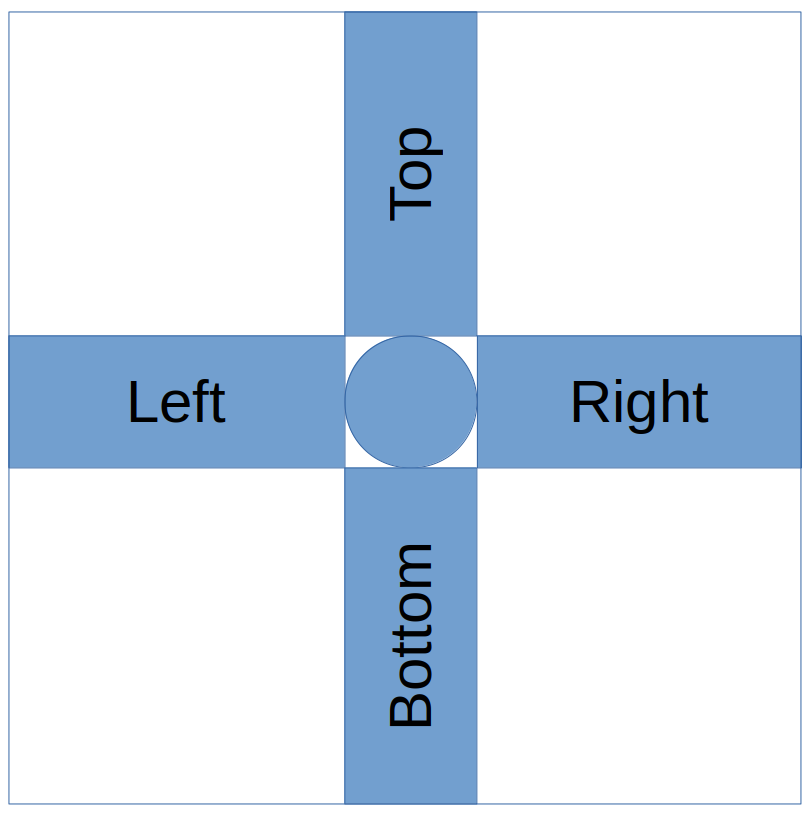
\includegraphics[width = 150pt]{images/rtlb}\\
					\caption{Scheme showing which parts of wall are added according to r,t,l,b values}
				\end{img}
				
			\dsubsection{Adding Sprites according to tile types}
				The following script is used to add Sprites to their respective groups. See section \ref{sprite-groups} for reference.
\begin{lstlisting} [language = Python]
def loadlevel(file):
	global level, coins_total, player
	# level-loading procedure with input of standard 32x32 bitmap level file
	level = readlevel(file)
	for col in range(0, resources.constants.gamesize):
		for row in range(0, resources.constants.gamesize):
			box = level[col][row]
			if box != resources.constants.leveldef["wall"] and box != resources.constants.leveldef['nothing']:
				eatable = Eatable(0, (col, row))
				eatables_list.add(eatable)
				coins_total += 1
			if box == resources.constants.leveldef["wall"]:
				wall = Wall((col, row), walltypecheck((col, row)))
				walls_list.add(wall)
			elif box == resources.constants.leveldef["player"]:
				player = Player((col, row))
			players_list.add(player)
			elif box == resources.constants.leveldef["red_ghost"]:
				ghost = Ghost((col, row), 'red')
				ghosts_list.add(ghost)
			elif box == resources.constants.leveldef["blue_ghost"]:
				ghost = Ghost((col, row), 'blue')
				ghosts_list.add(ghost)
			elif box == resources.constants.leveldef["green_ghost"]:
				ghost = Ghost((col, row), 'green')
				ghosts_list.add(ghost)
\end{lstlisting}
			\dsubsection{Sprite Groups}
				\label{sprite-groups}
				Within the main program file the following groups are globally declared.
\begin{lstlisting} [language = Python]
eatables_list = pygame.sprite.Group()
walls_list = pygame.sprite.Group()
players_list = pygame.sprite.Group()
ghosts_list = pygame.sprite.Group()
\end{lstlisting}
				Each of them stores Sprites of respective type - a very useful feature of pygame.sprite allowing manipulating multiple objects at once.
		\section{Ghost pathfinding algorithm}
			This section covers the most algorithmically complex part of this project - ghost pathfinding system. As seen in section \ref{ghost-movement} the concept is based on BFS graph search. But first there must be a graph to begin with. It's important to note that the graph is stored in 'thegraph' global variable - pretty descriptive, as this is the only graph implementation used in this project.
			\dsubsection{Graph structure}
				Formally - the graph is a list of lists of lists of lists of integers - notably complex structure. It's easier to imagine it though as a two-dimensional matrix of lists of tile locations - that sounds like something comprehensible by a human mind. Namely - first two iterable arguments are (x,y) coordinates of the tile we want to query for neighboring tiles. If we were to
				\begin{lstlisting} [language = Python]
print(thegraph[5][5])
				\end{lstlisting}
				we would see a list of points in [x,y] format, all tiles that a Movable could move to from tile (5,5).
			\dsubsection{Graph building}
				\begin{lstlisting} [language = Python]
def graphbuilder():
	global level, thegraph
	thegraph = [[[] for i in range(resources.constants.gamesize)] for j in range(resources.constants.gamesize)]
	for i in range(resources.constants.gamesize):
		for j in range(resources.constants.gamesize):
		# iterating through all tiles in the grid
			if level[i][j] != resources.constants.leveldef["wall"]:
			# taking advantage of the fact that Movables can move on all tiles that are not initially marked as walls
				location = [i, j]
				# processing location in more suitable format
				# and now, iterating through all possible neighbours of the processed tile (with checking if it isn't by any chance a border tile)
				if location[0] != 0:
					if level[location[0] - 1][location[1]] != resources.constants.leveldef["wall"]:
						thegraph[location[0]][location[1]] += [[location[0] - 1, location[1]]]
				if location[0] != resources.constants.gamesize-1:
					if level[location[0] + 1][location[1]] != resources.constants.leveldef["wall"]:
						thegraph[location[0]][location[1]] += [[location[0] + 1, location[1]]]
				if location[1] != 0:
					if level[location[0]][location[1] - 1] != resources.constants.leveldef["wall"]:
						thegraph[location[0]][location[1]] += [[location[0], location[1] - 1]]
				if location[1] != resources.constants.gamesize-1:
					if level[location[0]][location[1] + 1] != resources.constants.leveldef["wall"]:
						thegraph[location[0]][location[1]] += [[location[0], location[1] + 1]]
				\end{lstlisting}
				As seen for every possible neighboring tile the algorithm checks whether it is a wall and if it's not - it adds it to the list of all tiles a Movable may move to. As walls do not move, appear nor disappear this structure remains static throughout the level and must only be processed once upon level loading.
			\dsubsection{Choosing a target tile for each ghost}
				As described in Section \ref{constants}, resources.constants.scatterSize governs to how distant tile should green and blue ghost move. But when we add let's say a vector (2,2) to player's location, there is no guarantee that this tile is not a wall. If it was a wall it wouldn't appear on any list of neighbors of surrounding tile - ghost wouldn't be able to move there. Worse, there is no guarantee that this tile is even within the boundaries of the game board. I have discovered it during first tests of ghost chasing - game crashed as internal algorithms tried to fetch neighbors of tile which coordinates were greater than board size - this resulted in indexError. Therefore a need for the following function appeared:
				\begin{lstlisting}[language = Python]
def find_nearest_not_wall(point):
	if point[0] > resources.constants.gamesize-1:
		point[0] = resources.constants.gamesize-1
	if point[0] < 0:
		point[0] = 0
	if point[1] > resources.constants.gamesize-1:
		point[1] = resources.constants.gamesize-1
	if point[1] < 0:
		point[1] = 0
	if level[point[0]][point[1]] != resources.constants.leveldef['wall']:
		return point
	radius = 1
	while True:
		for i in range(point[0]-radius, point[0]+radius):
			for j in range(point[1]-radius, point[1]+radius):
			try:
				if level[i][j] != resources.constants.leveldef['wall']:
					return [i, j]
			except IndexError:
				pass
		radius += 1
				\end{lstlisting}
				With a slightly deceiving name - find\_nearest\_not\_wall - not only finds the coordinates of the nearest tile that isn't marked as a wall but it finds the nearest tile that isn't marked as a wall \textbf{that actually exists}.
				Within lines 2-9 the location is being confined to the boundaries of the board - then condition in line 10 checks whether the tile in question is a wall - if it isn't - that solves the problem. Else - the actual search begins. With growing radius neighboring tiles are checked for not being a wall. As this algorithm may eventually lead to checking type of a tile outside the board, a try/catch routine is used. By filtering cases of IndexError, nonexistent tiles aren't checked. I found this solution cleaner that limiting the borders of search, checking whether radius doesn't extend beyond the board, after all it's only 3 very clean lines. The function eventually returns a nearest existing point not being a wall.
			\dsubsection{Actual pathfinding}
				\label{pathfinding}
				After giving it a thought, the ghosts don't really require a complete path to operate. They just need to know where next to move. One single tile location or even a direction. I also figured that running searches from each tile of ghost's neighbors is inefficient. Out of pure reason... What seems faster? Finding one needle in a haystack three times or finding one of three needles in a haystack once? I would go for the second one. Here are two diagrams illustrating the concept:
				\begin{img}
					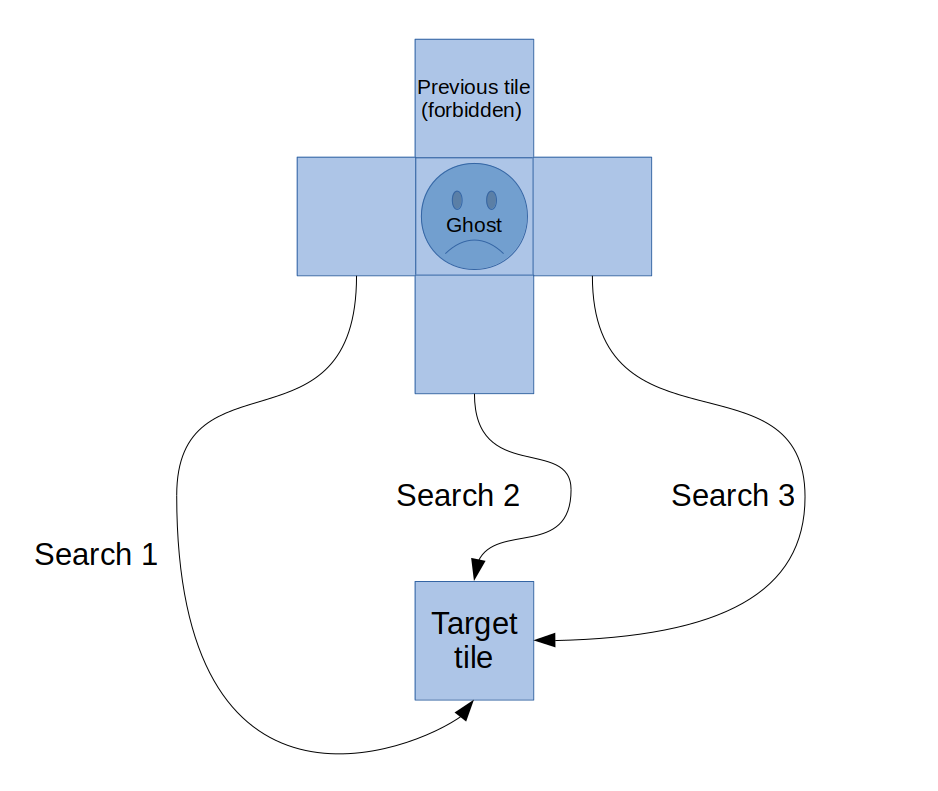
\includegraphics[width=400pt]{images/3searches}\\
					\caption{Inefficient method of running three searches.}
				\end{img}
				\begin{img}
					\includegraphics[width=300pt]{images/1search}\\
					\caption{Efficient method of running one search.}
				\end{img}
				To keep things simple, my algorithm for pathfinding accepts three arguments: start (ghost position), end(target tile position) and forbidden (tile the ghost moved from - ghost reversing prevention as per requirement \ref{req-ghost-not-reversing}).
				The initial version of the code had the following form.
				\begin{lstlisting}[language=Python]
def find_next_move(start, end):
	visited = []
	queue = []
	end = find_nearest_not_wall(end)
	# as start is guaranteed not to be wall, both ends are now places a Movable may move to
	neighbours = thegraph[start[0]][start[1]]
	queue.append(end)
	visited.append(end)
	for point in queue:
		if point in neighbours:
			return point
		for node in thegraph[point[0]][point[1]]:
			if node not in visited:
				visited.append(node)
				queue.append(node)
				\end{lstlisting}
				While this algorithm actually produced solutions in the initial testing stage, it was slow and I realized it didn't comply with Requirement \ref{req-ghost-not-reversing}. To address these issues, changes were made and now the code for the main pathfinding function is as follows:
				\begin{lstlisting} [language = Python]
def find_next_move(start, end, forbidden):
	visited = []
	# storing visited nodes
	queue = []
	# storing nodes to visit
	end = find_nearest_not_wall(end)
	# as start is guaranteed not to be wall, both ends are now places a Movable may move to
	neighbours = thegraph[start[0]][start[1]].copy()
	# preventing corrupting thegraph when excluding forbidden tile
	try:
		# try as forbidden tile may be any tile after reset
		# particularly it may not be in neighbors
		neighbours.remove([forbidden[0], forbidden[1]])
		# removing forbidden tile from neighbors
	except Exception:
		pass
	queue.append([end[0], end[1]])
	# start search from the end (target tile)
	visited.append(end)
	# mark end as a visited node
	for point in queue:
		if point not in visited:
			visited.append(point)
			# mark current point as visited
		if point in neighbours:
			return point
			# if solution is find return next tile for the ghost
		for node in thegraph[point[0]][point[1]]:
			if node not in visited and node != [forbidden[0], forbidden[1]]:
				queue.append(node)
				# add all unvisited neighbors of current node to the queue
				\end{lstlisting}
Being a rather clean BFS implementation this code returns only the location of one of ghost's neighbors - the tile it has to move to next. It was rewritten from scratch and well commented. Forbidden tile was added and therefore Requirement \ref{req-ghost-not-reversing} fulfilled.
		\section{Designing resources}
			Admittedly, my computer graphics skills are quite limited, so are manual. I considered designing graphics on paper, scanning them and importing into game. Following my first sketches I have decided to rather use GIMP instead of paper and pencils. Even though, some initial drawings on a whiteboard came handy.\\
			\begin{img}
				\includegraphics[width=300pt]{images/wall-whiteboard-design.jpg}\\
				\caption{Initial whiteboard design of the wall tiles}
			\end{img}
			As per Requirement \ref{req-orig-colors}, I needed to produce designs similar to those in original PacMan.
			\begin{img}
				\includegraphics[width=300pt]{images/original-graphics.jpg}\\
				\caption{Original PacMan graphics. Source: www.todayifoundout.com}
			\end{img}
			\dsubsection{Walls}
				These were rather simple. While original PacMan walls were build with a double blue framework, I went for a single framework. There is a clearly justified reason for that - my game was initially bigger and if I were to have double framework walls, player might have become confused, whether some space is accessible or not. After all the game board is a maze. I started with the simplest walls - 1010 and 0101. See pictures in the Design Section \ref{walls}. Then I generated a simple 1100 arc. Rest of the arcs were just rotated versions of it. Walls with three 1s and one 0 in their code, resembling letter T, were just merges of two of those double 1s arcs and wall 1111 was a merger of them all. GIMP offered tools for easy rotation and cop-pasting, which led to the graphics being produced in no time. I had to figure out how to make them transparent so that the game background could be seen from underneath. Again, GIMP offered function "Background to Alpha" which solved the problem instantly. And last, the format - it had to support transparency, be quite compact and readable by Pygame. I turned to GIF as it fitted these requirements perfectly.
			\dsubsection{Ghosts}
				In my opinion PycMan's greatest advantage is its simplicity - ghosts were created using GIMP's spray tool while pretty randomly stroking laptop's touchpad. This gave them their unique shape. To produce three ghosts of the same shape and different colors I used color manipulation tools available within GIMP to alter RGB channels in the original picture. Again these were exported as GIFs to preserve the partial transparency. For ghost graphic in red see Figure \ref{ghostimage}.
			\dsubsection{Player}
				The under-appreciated GIMP's ability to create circles of a single color and its unprecedented selection tool were used to create player's graphic of a yellow ball with 'mouth', fulfilling Requirement \ref{req-player-shape}. Again this was exported as GIF to preserve the Alpha channel.
		\section{Core program code}
			\dsubsection{Playing a single level}
				To initialize the game, the core program calls function playlevel(), which takes no arguments as it utilizes global variables for reference on which level should be played and on lives remaining.
				\begin{lstlisting} [language = Python]
def playlevel():
	global coins_eaten, coins_total, lives, levelno
	# marking variables as global
	coins_total = coins_eaten = 0
	# resetting coin counters
	prepare_level(resources.paths.levelorder[levelno])
	# level loading
	game_on = True
	# game starter
	clock = pygame.time.Clock()
	# clock init
	eatables_list.update()
	walls_list.update()
	players_list.update()
	ghosts_list.update()
	# updating Sprite Groups
	player_time_segment = resources.constants.playerTimeSegmentSize
	ghost_time_segment = resources.constants.ghostTimeSegmentSize
	# forcing pathfinding to update
				\end{lstlisting}
				By this part all initialization is done and the program starts main game loop.
				\subsubsection{Main loop}
					Following code initializes the main while loop. Its execution finishes when some part of the program sets game\_on flag to False.
					\begin{lstlisting} [language = Python]
# ----- Main game loop -----
while game_on:
					\end{lstlisting}
				\subsubsection{Handling completing the level}
					The following code executes when all coins are eaten. It switches the game to next level and prevents next loop execution by setting the game\_on flag to False. This fulfills Requirement \ref{req-level-up}
					\begin{lstlisting} [language = Python]
# ----- Level - winning handling -----
if coins_eaten == coins_total:
	levelno += 1
	game_on = False
	# ----- stop the level if all coins are eaten -----
					\end{lstlisting}
				\subsubsection{Handling user input and movement part 1}
					The following snippet executes only once per Player's Time Segment. It checks for user input, whether the game window was closed using operating system infrastructure and processes player's surroundings to determine to which tiles user can move (not to move onto wall tile as per Requirement \ref{req-walls-not-passable}).
					\begin{lstlisting} [language = Python]
if player_time_segment == resources.constants.playerTimeSegmentSize:
	# ----- Handling user input pt1 ------
	for event in pygame.event.get():
		if event.type == pygame.QUIT:
			game_on = False

	# ----- checking pressed keys -----
	keys = pygame.key.get_pressed()
	# ----- wall collision check -----
	surroundings = walltypecheck(player.location)
					\end{lstlisting}
				\subsubsection{Handling ghost movement part 1}
					This code, executed once per Ghosts' Time Segment assigns new target tiles for each ghost using pathfinding function described in Section \ref{pathfinding}, implementing changes to target tiles form Section \ref{hunting}, fulfilling Requirement \ref{req-ghost-differences} and \ref{req-ghost-movement}.
					\begin{lstlisting} [language = Python]
# ----- ghost movement handling pt 1 -----
if ghost_time_segment == resources.constants.ghostTimeSegmentSize:
	# if it's time to update paths update them
	for ghost in ghosts_list.sprites():
		if ghost.color == 'red':
			ghost.nexttile = find_next_move(ghost.location, player.location, ghost.previouslocation)
		elif ghost.color == 'blue':
			ghost.nexttile = find_next_move(ghost.location,
			[player.location[0] + resources.constants.scatterSize,
			player.location[1] + resources.constants.scatterSize],
			ghost.previouslocation)
		elif ghost.color == 'green':
			ghost.nexttile = find_next_move(ghost.location,
			[player.location[0] - resources.constants.scatterSize,
			player.location[1] - resources.constants.scatterSize],
			ghost.previouslocation)
					\end{lstlisting}
				\subsubsection{Updating 'part' counters}
					As Movable 'move' method requires supplying it with with Time Segment's Part, the following codes produces such number for both Ghosts (note that Ghosts share the same Time Segments)and the Player. For reference on Parts and Time Segments see Section \ref{timesegments}.
					\begin{lstlisting} [language = Python]
# ----- handling some frames/move -----
player_part = resources.constants.playerTimeSegmentSize - player_time_segment
ghost_part = resources.constants.ghostTimeSegmentSize - ghost_time_segment
					\end{lstlisting}
				\subsubsection{Handling input part 2}
					As actual user input occurs every Player's Time Segment, rather than every Part, the following code executes every part, to actually move the Player's sprite.
					\begin{lstlisting} [language = Python]
# ----- input handling pt 2 / player movement handling -----
if keys[pygame.K_LEFT] and surroundings[2] == '0':
	player.move('left', player_part)
elif keys[pygame.K_RIGHT] and surroundings[0] == '0':
	player.move('right', player_part)
elif keys[pygame.K_UP] and surroundings[1] == '0':
	player.move('up', player_part)
elif keys[pygame.K_DOWN] and surroundings[3] == '0':
	player.move('down', player_part)
					\end{lstlisting}
				\subsubsection{Handling ghost movement part 2}
					Same as with player, actual Sprites moving must occur every Part, rather than every Time Segment. This loop iterates through Ghosts and moves each of them.
					\begin{lstlisting} [language = Python]
# ----- ghost movement handling pt 2 -----
for ghost in ghosts_list.sprites():
	try:
		ghost.move((ghost.nexttile[0] - ghost.location[0], -ghost.nexttile[1] + ghost.location[1]), ghost_part)
	except Exception:
		# if for some unforseen reason it's impossible to move the ghost just leave it there
		pass
					\end{lstlisting}
				\subsubsection{Handling player dying}
					As per Requirement \ref{req-life-loss}, the game processes player dying by checking whether its current location matches any of the Ghosts' locations. If so, the life is subtracted from lives counter and the board is reseted. If the Player is subsequently in possession of no lives, game\_on flag is set to False to prevent next loop execution.
					\begin{lstlisting} [language = Python]
# ----- player dying handling -----
for ghost in ghosts_list.sprites():
	if ghost.location == player.location:
		# decrease lives counter
		lives -= 1
		reset()
		# reset the board
		player_time_segment = resources.constants.playerTimeSegmentSize+1
		ghost_time_segment = resources.constants.ghostTimeSegmentSize+1
		# force game to update ghost paths after respawning
if lives <= 0:
	# if the player is dead for good
	game_on = False
	break
					\end{lstlisting}
				\subsubsection{Drawing}
					Following code is used to render Sprites on the screen.
					\begin{lstlisting} [language = Python]
# ----- Updating sprites position -----
eatables_list.update()
walls_list.update()
players_list.update()
ghosts_list.update()
# ----- Fill screen with background -----
screen.fill(resources.colors.background)
# ----- ...and sprites -----
eatables_list.draw(screen)
walls_list.draw(screen)
players_list.draw(screen)
ghosts_list.draw(screen)
					\end{lstlisting}
				\subsubsection{Processing and rendering counters}
					This code handles counters displayed below the board.
					\begin{lstlisting} [language = Python]	
# ----- Counter info -----
label = myfont.render("Coins eaten " + str(coins_eaten) +" / " + str(coins_total) +
	"     Lives remaining " + str(lives) +
	"     Level " + str(levelno+1), 1, (255, 255, 0))
screen.blit(label, (resources.constants.tileWidth / 2, resources.constants.gamesize * resources.constants.tileWidth))
					\end{lstlisting}
				\subsubsection{Refreshing screen}
					The following code handles screen refreshing using pygame internal methods and supplies new values for player\_time\_segment and ghost\_time\_segment variables.
					\begin{lstlisting} [language = Python]
# ----- Refresh Screen -----
pygame.display.flip()

# ----- FPS handling -----
player_time_segment -= 1
ghost_time_segment -= 1
clock.tick(resources.constants.fps)
					\end{lstlisting}
				\subsubsection{Handling eating Eatables}
					As per Requirement \ref{req-coins-disappearing} and \ref{req-level-progress}, the following code checks whether any of the Eatables is affected by Player's presence and if so, it kills it, modifying appropriate counters.
					\begin{lstlisting} [language = Python]
# ----- eating handling -----
for eatable in eatables_list.sprites():
	if eatable.location == player.location:
		eatable.kill()
		if eatable.type == 'coin':
			coins_eaten += 1
			# increasing eaten points counter
		elif eatable.type == 'heart':
			lives += 1
			# increasing number of lives
					\end{lstlisting}
				\subsubsection{Initializing new Time Periods}
					Finally, if either of Time Segments comes to an end, the following code executes to initialize a new one.
					\begin{lstlisting} [language = Python]
# ----- initializing new time periods -----
if not player_time_segment:
	player_time_segment = resources.constants.playerTimeSegmentSize
if not ghost_time_segment:
	ghost_time_segment = resources.constants.ghostTimeSegmentSize
					\end{lstlisting}
				Provided the game\_on flag is still set to True, the loop continues.
				\linebreak
				
				Development of the code described in the above Section was particularly difficult due to having to simultaneously implement two Time Segment handlers. (See Section \ref{timesegments} for Time Segment explanation.)
				My first approach was to implement those within single counter. It worked but there was no way to satisfy Requirement \ref{req-player-faster}.
				Another problem I encountered was with the input handling. The player's sprite was jumping around, because player could change moving direction mid-time segment. The obvious choice was to move keypress checking to section that only executes once per time segment, rather than once per frame. My concern was that this will affect overall user input performance, compromising Requirement \ref{req-input}. My preliminary testing as well as $\beta$-testing revealed that with 60fps and player segment size equal to 10, the input rate of 6 key presses per second seemed optimal.
			\dsubsection{Function switching levels}
				\label{main}
				Function named main() taking no parameters, iterating through levels and displaying appropriate messages. This is the main function that launches the whole game. 
				\begin{lstlisting} [language = Python]
def main():
	show_message(resources.constants.tutorialStringList)
	while lives > 0 and levelno <= resources.constants.totallevels:
		print(levelno)
		playlevel()
		show_message(resources.constants.congratsStringList)
	if lives > 0:
		show_message(resources.constants.realCongratsStringList)
	else:
		show_message(resources.constants.theEndStringList)
				\end{lstlisting}
				When the while loop breaks, either Game Over screen is displayed or a congratulations screen, fulfilling Requirements \ref{req-messages}.
			\dsubsection{Displaying messages}
				As it's seen in the Section \ref{main} - the function show\_message is used to display small text messages on the screen. Those messages include:
				\begin{itemize}
					\item
						Tutorial screen
					\item
						Congratulations on completing a level
					\item
						A Game Over screen saying that the player lost
					\item
						Congratulations on completing the whole game
				\end{itemize}
				Following is the code for the show\_message function. It takes a single argument of a list of lines to display.
				\begin{lstlisting} [language = Python]
def show_message(messageboard):
	screen.fill(resources.colors.background)
	for i in range(len(messageboard)):
		label = myfont.render(messageboard[i], 1, (255, 255, 0))
		screen.blit(label, (0, resources.constants.fontsize * i))
	pygame.display.flip()
	waiting = True
	while waiting:
		for event in pygame.event.get():
			if event.type == pygame.KEYDOWN and event.key == 32:
				waiting = False
	sleep(0.05)
				\end{lstlisting}
	\chapter{Evaluation}
		The Implementation phase of project development is followed by Testing phase, during which the potentially ready project is checked for errors, functionality, usability and overall performance.
		\begin{img}
			\includegraphics[width=300pt]{images/tester.jpg}\\
			\caption{One of the testers playing PycMan}
		\end{img}
		\section{General testing}
			General testing involves mostly assessing game's responsiveness to various input, expected and unexpected under different initial conditions.
			The overall performance of the project satisfies both me and the stakeholder example, Wojciech, who did the $\beta$-testing.
			The game was tested under following conditions.\\
			\begin{center}
				\begin{tabular}{ | p{4cm} | p{4cm} | p{3cm} |}
					\hline
					Input&Response&Comment \\ \hline
					Performing mouse operations on the window&No response other than window closing when X button is clicked.&Expected response confirmed. \\ \hline
					Pressing keys other than arrow keys during gameplay&No response related to these keys&As expected, no action \\ \hline
					Pressing keys other than space bar when message is displayed&No response related to those keys&As expected, no action \\ \hline
					Pressing arrow keys repeatedly, very fast&Performance is not compromised, gameplay appears to be normal.&Acceptable response.\\ \hline
					Abandoning the game when it is on&The ghosts kill the player repeatedly and eventually the game comes to an end with the proper message displayed.&As expected, provided spacebar is pressed every kill\\ \hline
				\end{tabular}
			\end{center}
		\newpage
		\section{Meeting the requirements}
			\begin{center}
				\begin{longtable}{ | p{2cm} | p{5cm} | p{4cm} |}
					\hline
					Requirement&Testing method&Result \\ \hline
					\ref{req-orig-colors}&Game was visually assessed&The colors resemble these of original PacMan. \\ \hline
					\ref{req-player-shape}&Player's graphic was visually assessed.&Matches the requirement. \\ \hline
					\ref{req-player-rotation}&Game was played and player was moved&Player's sprite was rotated accordingly \\ \hline
					\ref{req-walls-not-passable}&Player was intentionally, excessively moved in direction of the wall, ghost movement was observed.&Neither of the sprites managed to pass the wall nor appear on the wall tile. \\ \hline
					\ref{req-ghost-movement}&Ghost movement was observed.&Ghosts appear to chase the player.\\ \hline
					\ref{req-life-loss}&Player was exposed to contact with the ghosts while stationary, moving away, sideways and towards the ghosts.&In a small number of cases the player was able to move 'through' the ghost when moving directly at it.\\ \hline
					\ref{req-reset}&The game was played and lives were lost.&Each time the loss of a life made the board reset.\\ \hline
					\ref{req-ghost-differences}&The ghosts were observed when the game was played.&Though ghosts sometimes took the same path, most of the time they were using different paths to surround the player.\\ \hline
					\ref{req-ghost-not-reversing}&The ghosts were observed when the game was played.&Ghosts didn't reverse. \\ \hline
					\ref{req-level-progress} \& \ref{req-coins-disappearing}&The game was played and the coins were exposed to the player.&Coins disappeared only upon contact and the appropriate counter increased. \\ \hline
					\ref{req-hearts} \& \ref{req-lifes++}&The game was played and the hearts were exposed to the player.&Hearts disappeared only upon contact and the appropriate counter increased. \\ \hline
					\ref{req-level-up} \& \ref{req-win} \& \ref{req-winnable}&The game was played to the end.&All levels were passable and upon game completion the appropriate message appeared.\\ \hline
					\ref{req-game-over}&The game was played and the player lost.&The appropriate message appeared when the number of lives fell below 0.\\ \hline
					\ref{req-messages}&The game was played and all conditions to display all messages were met.&Each time the messages appeared appropriately.\\ \hline
					\ref{req-smarter-ghosts}&The game was played. Assessors were also shown the original game.&Most of the testers named Pycman ghosts more intelligent\\ \hline
					\ref{req-no-ghost-house} \& \ref{req-no-powerips}&The game was played.&No ghost house, nor power-ups were found.\\ \hline
					\ref{req-not-dying}&The game was played.&No ghosts were harmed during testing.\\ \hline
					\ref{req-no-ghost-modes}&The game was played.&No behavior indicating any ghost 'modes' were found.\\ \hline
					\ref{req-player-faster}&The game was played. The speed of the sprites was observed.&Player was moving notably faster than the ghosts and was able to outrun them.\\ \hline
					\ref{req-input}&The arrow Keys were tested during the game.&Game was responsive to various combinations of pressed arrows and the game responded accordingly with no anomalies.\\ \hline
					\ref{req-spacebar}&The spacebar was used to dismiss the messages.&The messages disappeared accordingly.\\ \hline
					\ref{req-player-only-input}&The player was observed when no input was provided.&Player stayed still.\\ \hline
				\end{longtable}
			\end{center}
			Photos from testing as proof of features working:\\
			\begin{img}
				\includegraphics[width=300pt]{images/ghosts-chasing0.png}\\
				\caption{Image of ghosts chasing the player. Absence of eaten coins can be seen.}
			\end{img}
			\begin{img}
				\includegraphics[width=300pt]{images/hearts-working0.png}\\
				\caption{State of game prior to heart eating.}
			\end{img}
			\begin{img}
				\includegraphics[width=300pt]{images/hearts-working1.png}\\
				\caption{State of game post heart eating. Note the state of "Lives remaining" counter and the "Coins eaten" counter. 'Coins under the hearts' bug can be visible.}
				\label{coins-under-hearts}
			\end{img}
			
		\section{Changes}
			\dsubsection{Fixing requirement 1f}
				As seen above, Requirement \ref{req-life-loss} was not fully met as abnormal behavior was observed when the game was subject to rather atypical input. This is exactly why such a throughout testing was made. Further debugging indicated that Player was able to move through the ghost without losing life when following situation took place:\\
				\begin{itemize}
					\item The player is moving directly towards the ghost.
					\item When contact occurs, the frame number is divisible by both size of the player's and ghosts' time segment in frames.
				\end{itemize}
				Reason to this bug was order of commands in the main loop. The location of both player and ghosts was changed during a single execution of the main loop and only later the locations are checked for a collision. This allows a ghost and the player to 'swap' grid locations in a single frame without having the same location in time other than executions of the code in between the locations change. The solution to this problem was rather simple - the condition to check whether location of the ghost and the player are the same was moved there. the issue was fixed as indicated by further testing.
				
				The updated main loop code is as follows:
				\begin{lstlisting}[language=Python]
# ----- Main game loop -----
while game_on:
	# ----- Level - winning handling -----
	if coins_eaten == coins_total:
		levelno += 1
		game_on = False
		# ----- stop the level if all coins are eaten -----
	if player_time_segment == resources.constants.playerTimeSegmentSize:
		# ----- Handling user input pt1 ------
		for event in pygame.event.get():
			if event.type == pygame.QUIT:
				game_on = False
				exit(0)
		# ----- checking pressed keys -----
		keys = pygame.key.get_pressed()
		# ----- wall collision check -----
		surroundings = walltypecheck(player.location)

	# ----- ghost movement handling pt 1 -----
	if ghost_time_segment == resources.constants.ghostTimeSegmentSize:
		# if it's time to update paths update them
		for ghost in ghosts_list.sprites():
			if ghost.color == 'red':
				ghost.nexttile = find_next_move(ghost.location, player.location, ghost.previouslocation)
			elif ghost.color == 'blue':
				ghost.nexttile = find_next_move(ghost.location,
												[player.location[0] + resources.constants.scatterSize,
											 player.location[1] + resources.constants.scatterSize],
												ghost.previouslocation)
			elif ghost.color == 'green':
				ghost.nexttile = find_next_move(ghost.location,
												[player.location[0] - resources.constants.scatterSize,
											 player.location[1] - resources.constants.scatterSize],
												ghost.previouslocation)

	# ----- handling some frames/move -----
	player_part = resources.constants.playerTimeSegmentSize - player_time_segment
	ghost_part = resources.constants.ghostTimeSegmentSize - ghost_time_segment

	# ----- input handling pt 2 / player movement handling -----
	if keys[pygame.K_LEFT] and surroundings[2] == '0':
		player.move('left', player_part)
	elif keys[pygame.K_RIGHT] and surroundings[0] == '0':
		player.move('right', player_part)
	elif keys[pygame.K_UP] and surroundings[1] == '0':
		player.move('up', player_part)
	elif keys[pygame.K_DOWN] and surroundings[3] == '0':
		player.move('down', player_part)

	# ----- player dying handling -----
	for ghost in ghosts_list.sprites():
		if ghost.location == player.location:
			# decrease lives counter
			lives -= 1
			reset()
			# reset the board
			player_time_segment = resources.constants.playerTimeSegmentSize + 1
			ghost_time_segment = resources.constants.ghostTimeSegmentSize + 1
			# force game to update ghost paths after respawning

	# ----- ghost movement handling pt 2 -----
	for ghost in ghosts_list.sprites():
		try:
			ghost.move((ghost.nexttile[0] - ghost.location[0], -ghost.nexttile[1] + ghost.location[1]), ghost_part)
		except Exception:
			# if for some unforseen reason it's impossible to move the ghost just leave it there
			pass

	if lives <= 0:
		# if the player is dead for good
		break

	# ----- Updating sprites position -----
	eatables_list.update()
	walls_list.update()
	players_list.update()
	ghosts_list.update()
	# ----- Fill screen with background -----
	screen.fill(resources.colors.background)
	# ----- ...and sprites -----
	eatables_list.draw(screen)
	walls_list.draw(screen)
	players_list.draw(screen)
	ghosts_list.draw(screen)

	# ----- Counter info -----
	label = myfont.render("Coins eaten " + str(coins_eaten) + " / " + str(coins_total) +
				  "     Lives remaining " + str(lives) +
				  "     Level " + str(levelno+1), 1, (255, 255, 0))
	screen.blit(label, (resources.constants.tileWidth / 2, resources.constants.gamesize * resources.constants.tileWidth))

	# ----- Refresh Screen -----
	pygame.display.flip()

	# ----- FPS handling -----
	player_time_segment -= 1
	ghost_time_segment -= 1
	clock.tick(resources.constants.fps)

	# ----- eating handling -----
	for eatable in eatables_list.sprites():
		if eatable.location == player.location:
			eatable.kill()
			if eatable.type == 'coin':
				coins_eaten += 1
				# increasing eaten points counter
			elif eatable.type == 'heart':
				lives += 1
				# increasing number of lives

	# ----- initializing new time periods -----
	if not player_time_segment:
		player_time_segment = resources.constants.playerTimeSegmentSize
	if not ghost_time_segment:
		ghost_time_segment = resources.constants.ghostTimeSegmentSize
				\end{lstlisting}
			\dsubsection{'Coins under hearts' bug}
				During testing and as seen in the Figure \ref{coins-under-hearts}, the bug that places coins under hearts has been spotted. Its origin was backtracked to the original coin-placing function which was implemented prior to hearts development and therefore didn't account for them. Following is the code that placed coins in every tile which wasn't a 'wall' or marked as 'nothing'. This included tiles designated as 'hearts'.
				\begin{lstlisting}[language=Python]
box = level[col][row]
if box != resources.constants.leveldef["wall"]\
		and box != resources.constants.leveldef['nothing']:
	eatable = Eatable('coin', (col, row))
	eatables_list.add(eatable)
	coins_total += 1
				\end{lstlisting}
				The fix was easily developed and 'heart' tiles were added to the list of excluded tiles.
				\begin{lstlisting}[language=Python]
box = level[col][row]
if box != resources.constants.leveldef["wall"]\
		and box != resources.constants.leveldef['nothing']\
		and box != resources.constants.leveldef['heart']:
	eatable = Eatable('coin', (col, row))
	eatables_list.add(eatable)
	coins_total += 1
				\end{lstlisting}
				\begin{img}
					\includegraphics[width=300pt]{images/hearts-working2.png}\\
					\caption{State of game prior to heart eating.}
				\end{img}
				\begin{img}
					\includegraphics[width=300pt]{images/hearts-working3.png}\\
					\caption{State of game after heart eating. Note that the 'Coins eaten' counter was not increased, which is the expected behavior.}
				\end{img}
		\section{Room for future development}
			The game was tested on a personal laptop with rather mediocre specifications. It performed very well, though when framerate was measured I have identified the performance bottleneck to be the pathfinding algorithm. I have figured that there are at lest two very related ways of fixing its performance. As player chooses the next tile every time Period, the next pathfinding computation can begin immediately following this decision in a separate thread. This leads to obvious improvement of running the game in the total number of four threads. One main thread for displaying the graphics and providing general gameplay as well as handling the input + total of three threads, one per ghost for pathfinding. This would allow to run the game on processors with less computing power but could possibly make the project require more primary memory.
			
			The general structure of the project and its cleanness allows for non-obvious user modifications, adding new ghosts, hunting in different regions would require mere extra 10 lines or even less. The possibilities are unlimited as it is an Open Source project. But for the easiest start - users may create their own levels as a form of customizing the game.
			
			This game may be referred to as 'skinnable' - users may change the graphics as they wish by a matter of a simple files substitution. For example, the player's image can be substituted with the user face and ghosts may be substituted with images of college tuition invoices. Possibilities are endless though limited to 16 million colors bitmaps of size 64x64. 
		\section{Final assessment}
			The game appears to be working as expected, all assumed conditions were objectively met without major issues, no complaints were made other than that the game is hard which was actually intended.
		\section{Discussion}
			Admittedly the development of such project required some assumptions on how to approach the general problem of actually not wasting 20\% worth of A-Levels CS marks as well as learning something useful and presenting a quality work. Initial decisions that I have appreciated when beginning to develop this project include:
			\begin{itemize}
				\item
				Using \LaTeX\ instead of any popular word processor which broadened my knowledge on how to use this tool which will be an obvious choice later in my astronomy related future.
				\item
				Writing a clean code. The development of this project was not continuous, I joined English education system straight into Year 13 without knowing that I would have to make up for all the project work my peers already did over the Year 12 and holidays in between. This plus an exceptional amount of other work made me spread the development into large batches of sleep deprived weekend nights, without clean code I would have to spend extra time getting around undocumented solutions each time I attempted to move the project forward.
				\item
				Regular backups - honestly, these saved tens of hours when I corrupted my main drive.
				\item
				Doing something I know how to approach - yes, making a game was a challenge but then I knew what tools to use and when I stumbled on a problem I knew where to seek answers.
			\end{itemize}
		Things I would have done differently:
			\begin{itemize}
				\item
				I have said that \LaTeX was a good choice over for example Microsoft Word. Which still doesn't make it the perfect choice for documenting a Python project. There is a module for that (like for almost everything else). Jupyter Notebook would be my choice for writing this document if I were to do it again.
				\item
				Spending more time to figure out how to save time. I have spent definitely too much time on writing this documentation and I probably should have planned it better.
				\item
				Realizing that giving up on a feature is more painful than implementing it. Hearts were to vanish but then the cleanness of my OOP code made them appear in just a few lines.  
			\end{itemize}
	\chapter{Code appendix}
	TODO: update these files before final submission
		\section{main.py}
			\begin{lstlisting} [language = Python]
from classes import *
import resources
from levelprocesser import readlevel
from time import sleep
player = None
coins_total = 0
coins_eaten = 0
level = None
levelno = 0
lives = 30
pygame.init()
myfont = pygame.font.SysFont("monospace", resources.constants.fontsize)
pygame.display.set_caption("PycMan by Jan Dziedzic (13MF2)")
screen = pygame.display.set_mode(resources.constants.windowSize)

# ----- This 2D array holds info on location lists accessible (common edge) from tile represented by address -----
thegraph = [[[] for i in range(resources.constants.gamesize)] for j in range(resources.constants.gamesize)]


def walltypecheck(location):
	r = t = l = b = 0
	if location[0] != 0:
		if level[location[0]-1][location[1]] == resources.constants.leveldef["wall"]:
			l = 1
	if location[0] != resources.constants.gamesize-1:
		if level[location[0]+1][location[1]] == resources.constants.leveldef["wall"]:
			r = 1
	if location[1] != 0:
		if level[location[0]][location[1]-1] == resources.constants.leveldef["wall"]:
			t = 1
	if location[1] != resources.constants.gamesize-1:
		if level[location[0]][location[1]+1] == resources.constants.leveldef["wall"]:
			b = 1
	return str(r) + str(t) + str(l) + str(b)


# ----- Graphing stuff (for pathfinding) -----


def graphbuilder():
	global level, thegraph
	thegraph = [[[] for i in range(resources.constants.gamesize)] for j in range(resources.constants.gamesize)]
	for i in range(resources.constants.gamesize):
		for j in range(resources.constants.gamesize):
			# iterating through all tiles in the grid
			if level[i][j] != resources.constants.leveldef["wall"]:
				# taking advantage of the fact that Movables can move on all tiles that are not initially marked as walls
				location = [i, j]
				# and now, iterating through all possible neighbours of the processed tile (with checking if it isn't by any chance a border tile)
				if location[0] != 0:
					if level[location[0] - 1][location[1]] != resources.constants.leveldef["wall"]:
						thegraph[location[0]][location[1]] += [[location[0] - 1, location[1]]]
				if location[0] != resources.constants.gamesize-1:
					if level[location[0] + 1][location[1]] != resources.constants.leveldef["wall"]:
						thegraph[location[0]][location[1]] += [[location[0] + 1, location[1]]]
				if location[1] != 0:
					if level[location[0]][location[1] - 1] != resources.constants.leveldef["wall"]:
						thegraph[location[0]][location[1]] += [[location[0], location[1] - 1]]
				if location[1] != resources.constants.gamesize-1:
					if level[location[0]][location[1] + 1] != resources.constants.leveldef["wall"]:
						thegraph[location[0]][location[1]] += [[location[0], location[1] + 1]]


def find_nearest_not_wall(point):
	if point[0] > resources.constants.gamesize-1:
		point[0] = resources.constants.gamesize-1
	if point[0] < 0:
		point[0] = 0
	if point[1] > resources.constants.gamesize-1:
		point[1] = resources.constants.gamesize-1
	if point[1] < 0:
		point[1] = 0
	radius = 1
	if level[point[0]][point[1]] != resources.constants.leveldef['wall']:
		return point
	while True:
		for i in range(point[0]-radius, point[0]+radius):
			for j in range(point[1]-radius, point[1]+radius):
				try:
					if level[i][j] != resources.constants.leveldef['wall']:
						return [i, j]
				except IndexError:
					pass
		radius += 1


def find_next_move(start, end, forbidden):
	visited = []
	# storing visited nodes
	queue = []
	# storing nodes to visit
	end = find_nearest_not_wall(end)
	# as start is guaranteed not to be wall, both ends are now places a Movable may move to
	neighbours = thegraph[start[0]][start[1]].copy()
	# preventing corrupting thegraph when excluding forbidden tile
	try:
		# try as forbidden tile may be any tile after reset
		# particularly it may not be in neighbors
		neighbours.remove([forbidden[0], forbidden[1]])
		# removing forbidden tile from neighbors
	except Exception:
		pass
	queue.append([end[0], end[1]])
	# start search from the end (target tile)
	visited.append(end)
	# mark end as a visited node
	for point in queue:
		if point not in visited:
			visited.append(point)
			# mark current point as visited
		if point in neighbours:
			return point
			# if solution is find return next tile for the ghost
		for node in thegraph[point[0]][point[1]]:
			if node not in visited and node != [forbidden[0], forbidden[1]]:
				queue.append(node)
				# add all unvisited neighbors of current node to the queue


# ----- ----- -----


def loadlevel(file):
	global level, coins_total, player
	# level-loading procedure with input of standard 32x32 bitmap level file
	level = readlevel(file)
	for col in range(0, resources.constants.gamesize):
		for row in range(0, resources.constants.gamesize):
			box = level[col][row]
			if box != resources.constants.leveldef["wall"] and box != resources.constants.leveldef['nothing']:
				eatable = Eatable('coin', (col, row))
				eatables_list.add(eatable)
				coins_total += 1
			if box == resources.constants.leveldef["wall"]:
				wall = Wall((col, row), walltypecheck((col, row)))
				walls_list.add(wall)
			elif box == resources.constants.leveldef["player"]:
				player = Player((col, row))
				players_list.add(player)
			elif box == resources.constants.leveldef["red_ghost"]:
				redghost = Ghost((col, row), 'red')
				ghosts_list.add(redghost)
			elif box == resources.constants.leveldef["blue_ghost"]:
				redghost = Ghost((col, row), 'blue')
				ghosts_list.add(redghost)
			elif box == resources.constants.leveldef["green_ghost"]:
				redghost = Ghost((col, row), 'green')
				ghosts_list.add(redghost)


eatables_list = pygame.sprite.Group()
walls_list = pygame.sprite.Group()
players_list = pygame.sprite.Group()
ghosts_list = pygame.sprite.Group()


def prepare_level(levelfile):
	global eatables_list, walls_list, players_list, ghosts_list, player
	eatables_list = pygame.sprite.Group()
	walls_list = pygame.sprite.Group()
	players_list = pygame.sprite.Group()
	ghosts_list = pygame.sprite.Group()
	loadlevel(levelfile)
	graphbuilder()


def show_message(messageboard):
	screen.fill(resources.colors.background)
	for i in range(len(messageboard)):
		label = myfont.render(messageboard[i], 1, (255, 255, 0))
		screen.blit(label, (0, resources.constants.fontsize * i))
	pygame.display.flip()
	sleep(5)


def show_tutorial():
	show_message(resources.constants.tutorialStringList)


def show_congrats():
	screen.fill(resources.colors.background)
	for i in range(len(resources.constants.congratsStringList)):
		label = myfont.render(resources.constants.congratsStringList[i], 1, (255, 255, 0))
		screen.blit(label, (0, resources.constants.fontsize*i))
	pygame.display.flip()
	sleep(5)


def show_real_congrats():
	screen.fill(resources.colors.background)
	for i in range(len(resources.constants.realCongratsStringList)):
		label = myfont.render(resources.constants.realCongratsStringList[i], 1, (255, 255, 0))
		screen.blit(label, (0, resources.constants.fontsize*i))
	pygame.display.flip()
	sleep(5)

def show_permanent_death():
	screen.fill(resources.colors.background)
	for i in range(len(resources.constants.theEndStringList)):
		label = myfont.render(resources.constants.theEndStringList[i], 1, (255, 255, 0))
		screen.blit(label, (0, resources.constants.fontsize*i))
	pygame.display.flip()
	sleep(5)


def reset():
	for ghost in ghosts_list.sprites():
		ghost.reset()
	player.reset()


def playlevel():
	global coins_eaten, coins_total, lives, levelno, screen
	# marking variables as global
	coins_total = coins_eaten = 0
	# resetting coin counters
	prepare_level(resources.paths.levelorder[levelno])
	# level loading
	game_on = True
	# game starter
	clock = pygame.time.Clock()
	# clock init
	eatables_list.update()
	walls_list.update()
	players_list.update()
	ghosts_list.update()
	# updating Sprite Groups
	player_time_segment = resources.constants.playerTimeSegmentSize
	ghost_time_segment = resources.constants.ghostTimeSegmentSize
	# forcing pathfinding to update
	# ----- Main game loop -----
	while game_on:
		# ----- Level - winning handling -----
		if coins_eaten == coins_total:
			levelno += 1
			game_on = False
			# ----- stop the level if all coins are eaten -----
		if player_time_segment == resources.constants.playerTimeSegmentSize:
			# ----- Handling user input pt1 ------
			for event in pygame.event.get():
				if event.type == pygame.QUIT:
					game_on = False
					exit(0)
			# ----- checking pressed keys -----
			keys = pygame.key.get_pressed()
			# ----- wall collision check -----
			surroundings = walltypecheck(player.location)
		# ----- ghost movement handling pt 1 -----
		if ghost_time_segment == resources.constants.ghostTimeSegmentSize:
			# if it's time to update paths update them
			for ghost in ghosts_list.sprites():
				if ghost.color == 'red':
					ghost.nexttile = find_next_move(ghost.location, player.location, ghost.previouslocation)
				elif ghost.color == 'blue':
					ghost.nexttile = find_next_move(ghost.location,
													[player.location[0] + resources.constants.scatterSize,
													 player.location[1] + resources.constants.scatterSize],
													ghost.previouslocation)
				elif ghost.color == 'green':
					ghost.nexttile = find_next_move(ghost.location,
													[player.location[0] - resources.constants.scatterSize,
													 player.location[1] - resources.constants.scatterSize],
													ghost.previouslocation)

		# ----- handling some frames/move -----
		player_part = resources.constants.playerTimeSegmentSize - player_time_segment
		ghost_part = resources.constants.ghostTimeSegmentSize - ghost_time_segment

		# ----- input handling pt 2 / player movement handling -----
		if keys[pygame.K_LEFT] and surroundings[2] == '0':
			player.move('left', player_part)
		elif keys[pygame.K_RIGHT] and surroundings[0] == '0':
			player.move('right', player_part)
		elif keys[pygame.K_UP] and surroundings[1] == '0':
			player.move('up', player_part)
		elif keys[pygame.K_DOWN] and surroundings[3] == '0':
			player.move('down', player_part)

		# ----- ghost movement handling pt 2 -----
		for ghost in ghosts_list.sprites():
			try:
				ghost.move((ghost.nexttile[0] - ghost.location[0], -ghost.nexttile[1] + ghost.location[1]), ghost_part)
			except Exception:
				# if for some unforseen reason it's impossible to move the ghost just leave it there
				pass
		# ----- player dying handling -----
		for ghost in ghosts_list.sprites():
			if ghost.location == player.location:
				# decrease lives counter
				lives -= 1
				reset()
				# reset the board
				player_time_segment = resources.constants.playerTimeSegmentSize+1
				ghost_time_segment = resources.constants.ghostTimeSegmentSize+1
				# force game to update ghost paths after respawning
		if lives <= 0:
			# if the player is dead for good
			break

		# ----- Updating sprites position -----
		eatables_list.update()
		walls_list.update()
		players_list.update()
		ghosts_list.update()
		# ----- Fill screen with background -----
		screen.fill(resources.colors.background)
		# ----- ...and sprites -----
		eatables_list.draw(screen)
		walls_list.draw(screen)
		players_list.draw(screen)
		ghosts_list.draw(screen)

		# ----- Counter info -----
		label = myfont.render("Coins eaten " + str(coins_eaten) +" / " + str(coins_total) +
							  "	 Lives remaining " + str(lives) +
							  "	 Level " + str(levelno+1), 1, (255, 255, 0))
		screen.blit(label, (resources.constants.tileWidth / 2, resources.constants.gamesize * resources.constants.tileWidth))

		# ----- Refresh Screen -----
		pygame.display.flip()

		# ----- FPS handling -----
		player_time_segment -= 1
		ghost_time_segment -= 1
		clock.tick(resources.constants.fps)

		# ----- eating handling -----
		for eatable in eatables_list.sprites():
			if eatable.location == player.location:
				eatable.kill()
				coins_eaten += 1
				# increasing eaten points counter

		# ----- initializing new time periods -----
		if not player_time_segment:
			player_time_segment = resources.constants.playerTimeSegmentSize
		if not ghost_time_segment:
			ghost_time_segment = resources.constants.ghostTimeSegmentSize


def main():
	show_message(resources.constants.tutorialStringList)
	while lives > 0 and levelno <= resources.constants.totallevels:
		print(levelno)
		playlevel()
		show_message(resources.constants.congratsStringList)
	if lives > 0:
		show_message(resources.constants.realCongratsStringList)
	else:
		show_message(resources.constants.theEndStringList)

main()
			\end{lstlisting}
		\section{classes.py}
			\begin{lstlisting} [language = Python]
import pygame
import resources


class GameObject(pygame.sprite.Sprite):
	def __init__(self, location):
		super().__init__()
		self.image = None
		self.location = location
		self.initiallocation = location
		self.rect = None

	def setimage(self, image, size=resources.constants.tileSize, rotation=0):
		self.image = pygame.image.load(resources.paths.image[image])
		self.image = pygame.transform.scale(self.image, size)
		self.image = pygame.transform.rotate(self.image, rotation)
		self.rect = self.image.get_rect()
		self.rect.x, self.rect.y = self.location[0] * resources.constants.tileWidth, self.location[1] * resources.constants.tileWidth


class Eatable(GameObject):
	def __init__(self, type, location):
		super().__init__(location)
		self.type = type
		if type == "coin":
			self.setimage("coin", resources.constants.eatableSize)
		elif type == "heart":
			self.setimage("heart", resources.constants.eatableSize)


class Wall(GameObject):
	def __init__(self, location, type):
		super().__init__(location)
		self.setimage('w'+str(type))


class Movable(GameObject):
	def __init__(self, location):
		super().__init__(location)
		self.image = None
		self.speed = (0, 0)

	def setimage(self, image, size=resources.constants.movableSize, rotation=0):
		super().setimage(image, size, rotation)

	def move(self, direction, segmentsize, part=resources.constants.playerTimeSegmentSize - 1):
		if direction == 'up' or direction == (0, 1):
			self.speed = (0, -1)
		elif direction == 'down'or direction == (0, -1):
			self.speed = (0, 1)
		elif direction == 'left' or direction == (-1, 0):
			self.speed = (-1, 0)
		elif direction == 'right' or direction == (1, 0):
			self.speed = (1, 0)
		part2 = (part+1) / segmentsize
		self.rect.x, self.rect.y = (self.location[0] + self.speed[0] * resources.constants.speedFactor * part2) * resources.constants.tileWidth,\
								   (self.location[1] + self.speed[1] * resources.constants.speedFactor * part2) * resources.constants.tileWidth
		if part == segmentsize - 1:
			self.location = self.location[0] + self.speed[0] * resources.constants.speedFactor,\
							self.location[1] + self.speed[1] * resources.constants.speedFactor

	def reset(self):
		self.__init__(self.initiallocation)


class Player(Movable):
	def __init__(self, location):
		super().__init__(location)
		self.setimage('player', resources.constants.playerSize)

	def move(self, direction, part=resources.constants.playerTimeSegmentSize - 1, partsize=resources.constants.ghostTimeSegmentSize):
		rotation = 0
		if self.speed == (1, 0):
			rotation = 0
		elif self.speed == (-1, 0):
			rotation = 180
		elif self.speed == (0, -1):
			rotation = 90
		elif self.speed == (0, 1):
			rotation = 270
		super().setimage('player', resources.constants.playerSize, rotation)
		super().move(direction, segmentsize=resources.constants.playerTimeSegmentSize, part=part)


class Ghost(Movable):
	def __init__(self, location, color):
		super().__init__(location)
		self.color = color
		self.nexttile = None
		self.setimage(color+'_ghost')
		self.previouslocation = self.location

	def move(self, direction, part=resources.constants.ghostTimeSegmentSize - 1, partsize=resources.constants.ghostTimeSegmentSize):
		self.previouslocation = self.location
		super().move(direction, partsize, part)

	def reset(self):
		self.__init__(self.initiallocation, self.color)
			\end{lstlisting}
		\section{levelprocessor.py}
			\begin{lstlisting} [language = Python]
from PIL import Image
import resources


def readlevel(file):
	# level-loading procedure with input of gamesize^2 bitmap level file
	level = [[resources.constants.leveldef['nothing'] for i in range(resources.constants.gamesize)] for j in range(resources.constants.gamesize)]
	im = Image.open(resources.paths.levels + file)
	im.load()
	for col in range(0, resources.constants.gamesize):
		for row in range(0, resources.constants.gamesize):
			pixel = im.getpixel((col, row))
			if pixel == resources.constants.editordef["coin"]:
				level[col][row] = resources.constants.leveldef['coin']
			elif pixel == resources.constants.editordef["wall"]:
				level[col][row] = resources.constants.leveldef['wall']
			elif pixel == resources.constants.editordef["player"]:
				level[col][row] = resources.constants.leveldef['player']
			elif pixel == resources.constants.editordef["red_ghost"]:
				level[col][row] = resources.constants.leveldef['red_ghost']
			elif pixel == resources.constants.editordef["green_ghost"]:
				level[col][row] = resources.constants.leveldef['green_ghost']
			elif pixel == resources.constants.editordef["blue_ghost"]:
				level[col][row] = resources.constants.leveldef['blue_ghost']
	return level
			\end{lstlisting}
		\section{paths.py}
			\begin{lstlisting}[language = Python]
resources = "./resources/"
graphics = resources + "graphics/"
levels = resources + "levels/"

image = {
	"coin": graphics + "coin.png",
	"w0001": graphics + "w0001.gif",
	"w0010": graphics + "w0010.gif",
	"w0011": graphics + "w0011.gif",
	"w0100": graphics + "w0100.gif",
	"w0101": graphics + "w0101.gif",
	"w0110": graphics + "w0110.gif",
	"w0111": graphics + "w0111.gif",
	"w1000": graphics + "w1000.gif",
	"w1001": graphics + "w1001.gif",
	"w1010": graphics + "w1010.gif",
	"w1011": graphics + "w1011.gif",
	"w1100": graphics + "w1100.gif",
	"w1101": graphics + "w1101.gif",
	"w1110": graphics + "w1110.gif",
	"w1111": graphics + "w1111.gif",
	"player": graphics + "player.png",
	"red_ghost": graphics + "redghost.png",
	"blue_ghost": graphics + "blueghost.png",
	"green_ghost": graphics + "greenghost.png"
}

levelorder = [
	"level0.bmp",
	"level1.bmp",
	"level2.bmp",
	"level3.bmp",
	"level4.bmp",
	"level5.bmp",
	"level6.bmp"
]
			\end{lstlisting}
	\chapter{Levels appendix}
		\newpage
		\section{Level 1}
			\dsubsection{Source image}
			\begin{img}
				\includegraphics[width=350pt]{images/level1}\\
				\caption{Level 1 source image}
			\end{img}
			\dsubsection{Rendered level}
				\begin{img}
					\includegraphics[width=350pt]{images/level1_r}\\
					\caption{Level 1 rendered in game}
				\end{img}
		\section{Level 2}
			\dsubsection{Source image}
			\begin{img}
				\includegraphics[width=350pt]{images/level2}\\
				\caption{Level 2 source image}
			\end{img}
			\dsubsection{Rendered level}
			\begin{img}
				\includegraphics[width=350pt]{images/level2_r}\\
				\caption{Level 2 rendered in game}
			\end{img}
		\section{Level 3}
			\dsubsection{Source image}
			\begin{img}
				\includegraphics[width=350pt]{images/level3}\\
				\caption{Level 3 source image}
			\end{img}
			\dsubsection{Rendered level}
			\begin{img}
				\includegraphics[width=350pt]{images/level3_r}\\
				\caption{Level 3 rendered in game}
			\end{img}
		\section{Level 4}
			\dsubsection{Source image}
			\begin{img}
				\includegraphics[width=350pt]{images/level4}\\
				\caption{Level 4 source image}
			\end{img}
			\dsubsection{Rendered level}
			\begin{img}
				\includegraphics[width=350pt]{images/level4_r}\\
				\caption{Level 4 rendered in game}
			\end{img}
		\section{Level 5}
			\dsubsection{Source image}
			\begin{img}
				\includegraphics[width=350pt]{images/level5}\\
				\caption{Level 5 source image}
			\end{img}
			\dsubsection{Rendered level}
			\begin{img}
				\includegraphics[width=350pt]{images/level5_r}\\
				\caption{Level 5 rendered in game}
			\end{img}
		\section{Level 6}
			\dsubsection{Source image}
			\begin{img}
				\includegraphics[width=350pt]{images/level6}\\
				\caption{Level 6 source image}
			\end{img}
			\dsubsection{Rendered level}
			\begin{img}
				\includegraphics[width=350pt]{images/level6_r}\\
				\caption{Level 6 rendered in game}
			\end{img}
	\chapter{Guide to creating new levels}
		\label{new_levels_guide}
		Recommended software: GIMP version 2.3 or higher.\\
		Recommended hardware: screen, keyboard, mouse or a touch/stylus interface.
		\begin{itemize}
			\item
				Create a 32 x 32 RGB bitmap in .bmp format.
			\item
				Fill it with black color (255, 255, 255)
			\item
				Use pencil tool with a solid tip of size 1px to draw paths for the Movables, refer to Section \ref{level-permanent-storing} for available colors.
				It is strongly discouraged not to set border of the image as color black (255, 255, 255) symbolizing walls. While this shouldn't produce an error, this may negatively impact the gameplay.
			\item
				Again, use the same tool to place the player, ghosts, coins and hearts according to the above-mentioned specification.
				Remember that there should be precisely one player tile. You can add as many ghosts of all the three colors as you want. You may also decide not to include some.
			\item
				Place the bitmap in the resources/levels directory.
			\item
				Update 'totallevels' in recources/constants.py to indicate how many levels are in the folder.
			\item
				Add filename of your new level source image to 'levelorder' dictionary in resources/paths.py.
			\item
				Play your newly modified game!
		\end{itemize}
	\chapter{References}
		\begin{enumerate}
			\item
				https://goo.gl/36A62h
				\label{stronaopacmanie}
			\item
				https://www.pygame.org/docs
				\label{pygamedocs}
		\end{enumerate}
			
\end{document}
